%TODO : CHANGE THE FILE components/text.tex to include chapters

% Important: The shell-escape flag is required for the Minted package.
% Please compile this document with 'pdflatex -shell-escape main.tex'.
% If you are using another IDE, you may be able to specify this in the
% options or to provide an option like '% !TEX option = -shell-escape'
% in this file, depending on your builder. See the README.md for more.

% Don't put any content in here.
% Don't even include content files by using \input or \inlcude.
% Put your content into components/text.tex or include it there using \input.
% You probably want to modify the following files:
%   components/info.tex             contains the author, title etc.
%   components/settings.tex         contains the packages and settings.
%   components/commands.tex         contains helpful custom commands.
%   components/glossary.tex         contains an explanation of the used terms.
%   components/acknowledgements.tex contains the acknowledgements.
%   components/quote.tex            contains a quote.
%   components/abstract.tex         contains the abstract of the document.
%   components/text.tex             includes the actual content of the document.
%   components/outline.tex          contains the outline.
%   components/preface.tex          contains the preface.
%   chapters/                       contains the main text.
%   bibliography/literature.bib     contains the BibTeX entries.
%   images/                         contains all your content-related images.
%
% You probably don't need to change anything in the following files:
%   components/cover.tex            formats the front cover of the document.
%   components/titlepage.tex        formats the title page of the document.
%   components/disclaimer.tex       formats the disclaimer page.
%   styles/                         contains style elements (e.g. logos).
%   main.tex                        contains the top-level code structure.
%   README.md                       contains information about this template.

\documentclass[11pt,
              a4paper,
              index=totoc,
              headsepline,
              footsepline,
              BCOR=12mm,
              DIV=13]{scrbook}

% KOMA scrbook options:
%  index=totoc: include an entry for the index in the table of contents.
%  headsepline: use horizontal line under heading.
%  footsepline: use horizontal line above footer.
%  BCOR: binding correction (e.g.: BCOR=12mm)
%  DIV: Number of sheet sections (used for layout) (e.g.: DIV=13)


%  This code base is currently hosted at: 
%  https://github.com/waltsims/TUM_Thesis_Template_CSE
             
% !TEX root = ../main.tex
% Set here the title, authors and other stuff to be used for the cover
% This file is used by MAIN.TEX

% set title, authors and stuff for the cover
\def\university{Technische Universit{\"a}t M{\"u}nchen}
\def\universityLogo{styles/tum_logo}
\def\program{Computational Science and Engineering \\(International Master's Program)}
\def\programLogo{styles/cse_logo}
\def\doctype{Master's Thesis}

\def\title{Exploratory Analysis of Turbulent Flow Data using GNN-based Surrogate Model}
\def\author{Vaishali Ravishankar}
\def\examinerOne{Univ.-Prof.\ Dr.\ Hans Joachim Bungartz }
\def\examinerTwo{Prof.\ Dr.\ Jochen Garcke}
\def\assistantAdvisor{Kislaya Ravi}


\def\date{April 15th, 2023}

\def\keywords{{Graph Neural Network}, {Turbulence Model}}

% The following are used for the PDF metadata, by default the same as above.
\def\metaTitle{\title}
\def\metaAuthor{\author}
\def\metaSubject{\doctype\ -\ \university}
\def\metaKeywords{\keywords}

% text to appear in the footer
\def\footertext{}


% !TEX root = ../main.tex
% Included by MAIN.TEX

%--------------------------------------------------
% Fonts and page setup
%--------------------------------------------------

% Default font
\usepackage{palatino}

% Enable special PostScript fonts (optional)
% \usepackage{pifont}

% Manipulate the footer
\usepackage{scrlayer-scrpage}
\usepackage{scrhack}
\pagestyle{scrheadings}
\ifoot[\footertext]{\footertext} % \footertext set in INFO.TEX

% Set the font for the section headings
\renewcommand{\sectfont}{\normalfont \bfseries}

% Conditional commands in LaTeX documents, used for the \clearemptydoublepage.
\usepackage{ifthen}

% Typeset text in multiple columns (optional)
% \usepackage{multicol}

% Rotation tools, including rotated full-page floats (optional)
\usepackage{rotating}


%--------------------------------------------------
% Document structure
%--------------------------------------------------

% Pro­duce hy­per­text links in the doc­u­ment (recommended)
\usepackage{hyperref}

% Create glossaries and lists of acronyms
% depending on how many packages were shipped with your TeX distribution,
% you might need to install xindy. On Linux: sudo apt install xindy
\usepackage[toc,section=chapter, xindy, nomain]{glossaries}

% Define a glossary for acronyms
\newglossary[alg]{acronym}{acr}{acn}{Acronyms}

% Define a glossary for symbols
\newglossary[slg]{symbol}{sbl}{sbn}{Symbols}


% Standard LaTeX package for creating indexes
\usepackage{makeidx}


%--------------------------------------------------
% Bibliography
%--------------------------------------------------

% Set the bibliography style (default: plain)
\bibliographystyle{plain}

% Special biblography package (nice to have)
% \usepackage{natbib}


%--------------------------------------------------
% Graphics and floats
%--------------------------------------------------

% Enhanced support for graphics (recommended)
\usepackage{graphicx}
% Path to the figures directory (default: {figures/})
% Multiple entries are allowed, e.g. {{figures1/}{figures2/}}.
\graphicspath{{figures/}}

% Improved interface for floating objects (optional)
\usepackage{float}

% To use the subfigures (optional)
\usepackage{subcaption}


%--------------------------------------------------
% Mathematics
%--------------------------------------------------

% AMS mathematical facilities for LaTeX (recommended)
\usepackage{amsmath}

% TeX fonts from the American Mathematical Society (recommended)
\usepackage{amsfonts}

% Some extra math symbols (optional)
% \usepackage{amssymb}

% Extended maths fonts for LaTeX (optional)
% \usepackage{yhmath}

% Provide math delimiters whose size can be computed automatically (optional)
% \usepackage{commath}


%--------------------------------------------------
% Source code and algorithms
%--------------------------------------------------

% Source code typesetting
% \usepackage{listings} % (optional - alternative)
\usepackage[newfloat]{minted} % (recommended)
% Set global Minted options
\setminted{linenos, autogobble, frame=lines, framesep=2mm}
% Inline C++ (optional)
\newcommand{\incpp}[1]{\mintinline{c++}{#1}}
\newenvironment{code}{\captionsetup{type=listing}}{}
\SetupFloatingEnvironment{listing}{name=Source Code}

% Typeset algorithms - pseudocode (optional)
% \usepackage{algorithmicx}
% \usepackage{algpseudocode}
% Normal arrow comments
% \algrenewcommand{\algorithmiccomment}[1]{\hfill$\rightarrow$ #1}


%--------------------------------------------------
% Tables
%--------------------------------------------------

% Tables (optional)
\usepackage{tabu}

% Add color to LaTeX tables (optional)
\usepackage{colortbl}

% Create tabular cells spanning multiple rows (optional)
\usepackage{multirow}


%--------------------------------------------------
% Color
%--------------------------------------------------

% Use colors
\usepackage[dvipsnames]{xcolor}
% \usepackage[table]{xcolor}
% You may find all the pre-defined colors in
% https://en.wikibooks.org/wiki/LaTeX/Colors#Predefined_colors

% Custom colors
\definecolor{Pantone300C}{HTML}{0065BD} % TUM primary blue
\definecolor{Pantone301}{HTML}{005293}  % TUM secondary light blue
\definecolor{Pantone540}{HTML}{003359}  % TUM secondary dark blue
\definecolor{DarkGray}{HTML}{333333}    % TUM secondary dark gray
\definecolor{MediumGray}{HTML}{808080}  % TUM secondary medium gray
\definecolor{LightGray}{HTML}{CCCCC6}   % TUM secondary light gray
\definecolor{Pantone7527}{HTML}{DAD7CB} % TUM accent gray
\definecolor{Pantone158}{HTML}{E37222}  % TUM accent orange
\definecolor{Pantone383}{HTML}{A2AD00}  % TUM accent green
\definecolor{Pantone283}{HTML}{98C6EA}  % TUM accent very light blue
\definecolor{Pantone542}{HTML}{64A0C8}  % TUM accent light blue

% Color for the hyperlinks (e.g. table of contents)
\def\colorLinks{Pantone300C}
% Color for the web links
\def\colorUrl{Pantone542}
% Color for the citations
\def\colorCitations{Pantone158}

%--------------------------------------------------
% PDF output
%--------------------------------------------------

% Adjust the color of the links
\hypersetup{
  linkcolor=\colorLinks,%
  urlcolor=\colorUrl,%
  citecolor=\colorCitations
}

% Disable the coloring of the links when printing.
% Requires a compatible PDF reader.
\usepackage[ocgcolorlinks]{ocgx2}[2017/03/30]

% PDF Metadata
\hypersetup{
  pdftitle={\metaTitle},%
  pdfauthor={\metaAuthor},%
  pdfkeywords={\metaKeywords},%
  pdfsubject={\metaSubject}
}

% Create XMP Metadata (uses the values from hyperref)
\usepackage{hyperxmp}

% Make thumbnails (optional)
% \usepackage{thumbpdf}


%--------------------------------------------------
% Other settings
%--------------------------------------------------

% Define commands that appear not to eat spaces (optional)
\usepackage{xspace}


% !TEX root = ../main.tex
% Included by MAIN.TEX
% Please include your own cool commands here.
% Be only sure to comment it sufficiently so others can use it.

%-------------------------------------------------------------
%                      Own Commands
%-------------------------------------------------------------


%-------------------------------------------------------------
% math stuff -------------------------------------------------

% nice R, N, C
\newcommand{\nat}{\mathbb{N}}
\newcommand{\real}{\mathbb{R}}
\newcommand{\compl}{\mathbb{C}}

% un demi
\newcommand{\half}{\frac{1}{2}}

% parantheses
\newcommand{\parenth}[1]{ \left(#1 \right) }
\newcommand{\bracket}[1]{ \left[#1 \right] }
\newcommand{\accolade}[1]{ \left\{ #1 \right\} }
%\newcommand{\angle}[1]{ \left\langle  #1 \right\rangle }

% partial derivative: %#1 function, #2 which variable
% simple / single line version
\newcommand{\pardevS}[2]{ \delta_{#1} f(#2) }

% fraction version
\newcommand{\pardevF}[2]{ \frac{\partial #1}{\partial #2} }

% render vectors: 3 and 4 dimensional
\newcommand{\veciii}[3]{\left[ \begin{array}[h]{c} #1 \\ #2 \\ #3	\end{array} \right]}
\newcommand{\veciv}[4]{\left[ \begin{array}[h]{c} #1 \\ #2 \\ #3 \\ #4	\end{array} \right]}

% render matrices: 3  dimensional (arguments in row first order)
\newcommand{\matiii}[9]{\left[ \begin{array}[h]{ccc} #1 & #2 & #3 \\ #4 & #5 & #6 \\ #7 & #8 & #9	\end{array} \right]}

%-------------------------------------------------------------
% some abreviations ------------------------------------------
\newcommand{\Reg}{$^{\textregistered}$}
\newcommand{\reg}{$^{\textregistered}$ }
\newcommand{\Tm}{\texttrademark}
\newcommand{\tm}{\texttrademark~}
\newcommand {\bsl} {$\backslash$}

%-------------------------------------------------------------
% formating --------------------------------------------------

% Theorem & Co environments and counters
\newtheorem{theorem}{Theorem}[chapter]
\newtheorem{lemma}[theorem]{Lemma}
\newtheorem{corollary}[theorem]{Corollary}
\newtheorem{remark}[theorem]{Remark}
\newtheorem{definition}[theorem]{Definition}
\newtheorem{equat}[theorem]{Equation}
\newtheorem{example}[theorem]{Example}
%\newtheorem{algorithm}[theorem]{Algorithm}

% inserting figures
\newcommand{\insertfigure}[4]{ % Filename, Caption, Label, Width percent of textwidth
	\begin{figure}[htbp]
		\begin{center}
			\includegraphics[width=#4\textwidth]{#1}
		\end{center}
		\vspace{-0.4cm}
		\caption{#2}
		\label{#3}
	\end{figure}
}

% referecing figures

\newcommand{\refFigure}[1]{ %label
	Figure~\ref{#1}
}
\newcommand{\refChapter}[1]{ %label
	Chapter~\ref{#1}
}

\newcommand{\refSection}[1]{ %label
	Section~\ref{#1}
}

\newcommand{\refParagraph}[1]{ %label
	Paragraph~\ref{#1}
}

\newcommand{\refEquation}[1]{ %label
	Equation~\ref{#1}
}

\newcommand{\refTable}[1]{ %label
	Table~\ref{#1}
}

\newcommand{\rigidTransform}[2]
{
	${}^{#2}\!\mathbf{H}_{#1}$
}

% comment that appears on the border - very practical !!!
\newcommand{\comment}[1]{\marginpar{\raggedright \noindent \footnotesize {\textsl{#1}} }}

% page clearing
\newcommand{\clearemptydoublepage}{%
  \ifthenelse{\boolean{@twoside}}{\newpage{\pagestyle{empty}\cleardoublepage}}%
  {\clearpage}}

%-------------------------------------------------------------
%-------------------------------------------------------------

\newcommand{\etAl}{\emph{et al.}\mbox{ }}


% % !TEX root = ../main.tex
% \newacronym{RANS}{RANS}{Reynolds-Averaged Navier-Stokes}
% \newacronym{CNN}{CNN}{Convolutional Neural Network}

% \newacronym[longplural={partial differential equations}]{PDE}{PDE}{partial differential equations}
% \newacronym{mpi}{MPI}{Message Passing Interface}

% \newacronym[longplural={Random Walks on Spheres}]{RWoS}{RWoS}{Random Walk on Spheres}

% \newacronym[longplural={graphical processing units}]{GPU}{GPU}{Graphical Processing Unit}

% \newacronym[longplural={central processing units}]{CPU}{CPU}{central processing unit}

% \newacronym[longplural={arithmetic logic units}]{ALU}{ALU}{arithmetic logic unit}

% \newacronym[longplural={streaming multi-processors}]{SM}{SM}{streaming multi-processor}

% \newacronym[longplural={boundary value problems}]{BVP}{BVP}{boundary value problem}
% \newacronym[longplural={general purpose graphical processing units}]{GPGPU}{GPGPU}{general purpose graphical processing units}
% \newacronym{CUDA}{CUDA}{compute unified device architecture}
% \newacronym{RAM}{RAM}{random access memory}
% \newacronym{SRAM}{SRAM}{static random access memory}
% \newacronym{DRAM}{DRAM}{dynamic random access memory}
% \newacronym{I/O}{I/O}{input/output}
% \newacronym{PTX}{PTX}{Parallel Thread eXecution}
% \newacronym{jit}{JIT}{just in time}
\newglossaryentry{nut}{
  name={$\nu_t$},
  text={\ensuremath{\nu_t}},
  description={turbulent viscosity},
  type=symbol,
  sort=nu_t
}
\newglossaryentry{rho}
{
  name={$\rho$},
  text={\ensuremath{\rho}},
  description={Density of the fluid},
  type=symbol,
  sort=rho
}

\newglossaryentry{p}
{
  name={$\p$},
  text={\ensuremath{p}},
  description={Pressure},
  type=symbol,
  sort=p
}

\newglossaryentry{nu}
{
  name={$\nu$},
  text={\ensuremath{\nu}},
  description={Kinematic viscosity},
  type=symbol,
  sort=nu
}

\newglossaryentry{mu}
{
  name={$\mu$},
  text={\ensuremath{\mu}},
  description={Dynamic viscosity},
  type=symbol,
  sort=mu
}

\newglossaryentry{Sij}
{
  name={$\S_i_j$},
  text={\ensuremath{S_i_j}},
  description={Shear rate},
  type=symbol,
  sort=S_i_j
}

\newglossaryentry{mut}
{
  name={$\mu_t$},
  text={\ensuremath{\mu_t}},
  description={Turbulent viscosity},
  type=symbol,
  sort=mut
}

\newglossaryentry{k}
{
  name={$\k$},
  text={\ensuremath{k}},
  description={Turbulent kinetic energy},
  type=symbol,
  sort=k
}

\newglossaryentry{epsilon}
{
  name={$\epsilon$},
  text={\ensuremath{\epsilon}},
  description={Rate of dissipation of turbulent kinetic energy},
  type=symbol,
  sort=epsilon
}

\newglossaryentry{omega}
{
  name={$\omega$},
  text={\ensuremath{\omega}},
  description={Specific rate of turbulence dissipation},
  type=symbol,
  sort=omega
}

\newglossaryentry{x}
{
  name={$\x$},
  text={\ensuremath{x}},
  description={Input signals},
  type=symbol,
  sort=x
}

\newglossaryentry{w}
{
  name={$\w$},
  text={\ensuremath{w}},
  description={Weight vector},
  type=symbol,
  sort=w
}

\newglossaryentry{sigma}
{
  name={$\sigma$},
  text={\ensuremath{\sigma}},
  description={Activation function},
  type=symbol,
  sort=sigma
}

\newglossaryentry{b}
{
  name={$\b$},
  text={\ensuremath{b}},
  description={Bias},
  type=symbol,
  sort=x
}

\newglossaryentry{y}
{
  name={$\y$},
  text={\ensuremath{y}},
  description={Output},
  type=symbol,
  sort=y
}

\newglossaryentry{lambda}
{
  name={$\lambda$},
  text={\ensuremath{\lambda}},
  description={Regularization strength},
  type=symbol,
  sort=lamda
}

\newglossaryentry{muB}
{
  name={$\mu_B$},
  text={\ensuremath{\mu_B}},
  description={Mean of mini-batch B},
  type=symbol,
  sort=mu_B
}

\newglossaryentry{sigma2B}
{
  name={$\sigma^2_B$},
  text={\ensuremath{\sigma^2_B}},
  description={Variance of mini-batch B},
  type=symbol,
  sort=sigma2_B
}

\newglossaryentry{m}
{
  name={$\m$},
  text={\ensuremath{m}},
  description={Size of mini-batch},
  type=symbol,
  sort=m
}

\newglossaryentry{hatxi}
{
  name={$\hat{x}^i$},
  text={\ensuremath{\hat{x}^i}},
  description={Normalized input},
  type=symbol,
  sort=hatxi
}

\newglossaryentry{yi}
{
  name={$\y^i$},
  text={\ensuremath{y^i}},
  description={Output of batch normalization layer},
  type=symbol,
  sort=yi
}

\newglossaryentry{gamma}
{
  name={$\gamma$},
  text={\ensuremath{\gamma}},
  description={Scaling parameter},
  type=symbol,
  sort=gamma
}

\newglossaryentry{beta}
{
  name={$\beta$},
  text={\ensuremath{\beta}},
  description={Shifting parameter},
  type=symbol,
  sort=beta
}

\newglossaryentry{mathcall}
{
  name={$\mathcal{L}$},
  text={\ensuremath{\mathcal{L}}},
  description={Loss function},
  type=symbol,
  sort=mathcall
}

\newglossaryentry{theta}
{
  name={$\theta$},
  text={\ensuremath{\theta}},
  description={Parameters of the neural network being optimized},
  type=symbol,
  sort=theta
}

\newglossaryentry{N}
{
  name={$\N$},
  text={\ensuremath{N}},
  description={Sample size},
  type=symbol,
  sort=N
}

\newglossaryentry{eta}
{
  name={$\eta$},
  text={\ensuremath{\eta}},
  description={Learning rate},
  type=symbol,
  sort=eta
}


\newglossaryentry{hatmt}
{
  name={$\hat{m}_t$},
  text={\ensuremath{\hat{m}_t}},
  description={Bias-corrected first moment},
  type=symbol,
  sort=hatmt
}


\newglossaryentry{hatvt}
{
  name={$\hat{v}_t$},
  text={\ensuremath{\hat{v}_t}},
  description={Bias-corrected second moment},
  type=symbol,
  sort=hatvt
}


\newglossaryentry{X}
{
  name={$\X$},
  text={\ensuremath{X}},
  description={Node feature matrix},
  type=symbol,
  sort=X
}

\newglossaryentry{xi}
{
  name={$\x_i$},
  text={\ensuremath{x_i}},
  description={Feature vector},
  type=symbol,
  sort=xi
}

\newglossaryentry{vi}
{
  name={$\v_i$},
  text={\ensuremath{v_i}},
  description={Node i},
  type=symbol,
  sort=vi
}


\newacronym[type=acronym]{CAD}{CAD}{Computer-Aided Design}
\newacronym[type=acronym]{NSE}{NSE}{Navier-Stokes Equations}
\newacronym[type=acronym]{PDE}{PDE}{Partial Differential Equations}
\newacronym[type=acronym]{CFD}{CFD}{Computational Fluid Dynamics}
\newacronym[type=acronym]{DNS}{DNS}{Direct Numerical Simulation}
\newacronym[type=acronym]{ROM}{ROM}{Reduced Order Modelling}
\newacronym[type=acronym]{ML}{ML}{Machine Learning}
\newacronym[type=acronym]{DL}{DL}{Deep Learning}
\newacronym[type=acronym]{GNN}{GNN}{Graph Neural Networks}
\newacronym[type=acronym]{RANS}{RANS}{Reynolds Averaged Navier-Stokes}
\newacronym[type=acronym]{URANS}{URANS}{Unsteady Reynolds Averaged Navier-Stokes}
\newacronym[type=acronym]{LES}{LES}{Large Eddy Simulation}
\newacronym[type=acronym]{CNN}{CNN}{Convolutional Neural Networks}
\newacronym[type=acronym]{RNN}{RNN}{Recurrent Neural Networks}
\newacronym[type=acronym]{POD}{POD}{Proper Orthogonal Decomposition}
\newacronym[type=acronym]{PINN}{PINN}{Physics Informed Neural Networks}
\newacronym[type=acronym]{GMLS}{GMLS}{Generalized Moving Least Squares}
\newacronym[type=acronym]{GCNN}{GCNN}{Graph Convolutional Neural Networks}
\newacronym[type=acronym]{GCN}{GCN}{Graph Convolutional Networks}
\newacronym[type=acronym]{HOMER}{HOMER}{High-speed Orienting Momentum with Enhanced Reversibility}
\newacronym[type=acronym]{SST}{SST}{Shear Stress Transport}
\newacronym[type=acronym]{FDM}{FDM}{Finite Difference Method}
\newacronym[type=acronym]{FEM}{FEM}{Finite Element Method}
\newacronym[type=acronym]{FVM}{FVM}{Finite Volume Method}
\newacronym[type=acronym]{SIMPLE}{SIMPLE}{Semi Implicit Method for Pressure Linked Equations}
\newacronym[type=acronym]{ANN}{ANN}{Artificial Neural Networks}
\newacronym[type=acronym]{ReLU}{ReLU}{Rectified Linear Unit}
\newacronym[type=acronym]{NN}{NN}{Neural Networks}
\newacronym[type=acronym]{MLP}{MLP}{Multi Layer Perceptrons}
\newacronym[type=acronym]{SGD}{SGD}{Stochastic Gradient Descent}
\newacronym[type=acronym]{LOOCV}{LOOCV}{Leave One Out Cross-Validation}
\newacronym[type=acronym]{MSE}{MSE}{Mean Squared Error}
\newacronym[type=acronym]{RMSProp}{RMSProp}{Root Mean Squared Propagation}
\newacronym[type=acronym]{Adam}{Adam}{Adaptive Moment Estimation}
\newacronym[type=acronym]{AdaGrad}{AdaGrad}{Adaptive Gradient}
\newacronym[type=acronym]{MAE}{MAE}{Mean Absolute Error}
\newacronym[type=acronym]{RMSE}{RMSE}{Root Mean Squared Error}
\newacronym[type=acronym]{GAT}{GAT}{Graph ATtention Networks}
\newacronym[type=acronym]{COO}{COO}{Co-Ordinate list}
\newacronym[type=acronym]{MoNet}{MoNet}{Mixture Model Network}
\newacronym[type=acronym]{PCA}{PCA}{Principal Component Analysis}
\newacronym[type=acronym]{t-SNE}{t-SNE}{t-Distributed Stochastic Neighbor Embedding}
\newacronym[type=acronym]{DBSCAN}{DBSCAN}{Density-Based Spatial Clustering of Applications with Noise}
\newacronym[type=acronym]{k-NN}{k-NN}{k - Nearest Neighbors}
\newacronym[type=acronym]{HPC}{HPC}{High Performance Computing}
\newacronym[type=acronym]{GPU}{GPU}{Graphics Processing Unit}
\newacronym[type=acronym]{CPUs}{CPUs}{Central Processing Units}
\newacronym[type=acronym]{CPU}{CPU}{Central Processing Unit}
\newacronym[type=acronym]{SLURM}{SLURM}{Simple Linux Utility for Resource Management}


\makeglossaries

\begin{document}

 \frontmatter

 % !TEX root = ../main.tex
% The front cover.
% Included by MAIN.TEX

%--------------------------------------------------
% The Front Cover
%--------------------------------------------------

% correct BCOR - undo at the end !!!
\def\bcorcor{0.15cm}
\addtolength{\hoffset}{\bcorcor}

\thispagestyle{empty}

\vspace{4cm}
\begin{center}
	\includegraphics[width=4cm]{\universityLogo}\\
	\vspace{5mm}
	\huge \program \\
	\vspace{0.5cm}
	\large \university
\end{center}

\vspace{20mm}
\begin{center}
	{\Large \doctype}\\
	\vspace{20mm}
	{\huge \textbf \title}\\
	\vspace{15mm}
	{\LARGE  \author}\\
	\vspace{\fill}
	\includegraphics[width=4cm]{\programLogo}
\end{center}


 \clearemptydoublepage

 % !TEX root = ../main.tex
% The titlepage.
% Included by MAIN.TEX


%--------------------------------------------------
% The title page
%--------------------------------------------------

% correct BCOR - undo at the end !!!
\def\bcorcor{0.15cm}
\addtolength{\hoffset}{\bcorcor}

\thispagestyle{empty}

\vspace{4cm}
\begin{center}
    \includegraphics[width=4cm]{\universityLogo}\\
    \vspace{5mm}
    \huge \program \\
    \vspace{0.5cm}
    \large \university
\end{center}

\vspace{10mm}
\begin{center}
    {\Large \doctype}\\
    \vspace{10mm}
    {\LARGE \title}\\
    \vspace{10mm}

    \begin{tabular}{ll}
      \Large Author:                        & \Large \author \\[2mm]
      \Large 1\textsuperscript{st} examiner:& \Large \examinerOne\\[2mm]
      \Large 2\textsuperscript{nd} examiner:& \Large \examinerTwo \\[2mm]
      \Large Assistant advisor:             & \Large \assistantAdvisor \\[2mm]
      \Large Submission Date:               & \Large \date
    \end{tabular}

    \vspace{\fill}
    \includegraphics[width=4cm]{\programLogo}
\end{center}

% undo BCOR correction
\addtolength{\hoffset}{\bcorcor}


 % !TEX root = ../main.tex
\clearemptydoublepage

\thispagestyle{empty}
\vspace*{0.8\textheight}
\noindent
I hereby declare that this thesis is entirely the result of my own work except where otherwise indicated. I have only used the resources given in the list of references.

\vspace{15mm}
\noindent
\date \hspace{5cm} \author
\newpage


 % !TEX root = ../main.tex
\clearemptydoublepage
\phantomsection
\addcontentsline{toc}{chapter}{Acknowledgements}

\vspace*{2cm}

\begin{center}
{\Large \textbf{Acknowledgments}}
\end{center}

\vspace{1cm}

% \begin{center}
% I would like to thank Christian and Arno for their support and guidance throughout the 
% As I sit down to pen the acknowledgments for this thesis, I find myself reflecting on the journey that has been; a journey paved with challenges, learning, and immense support from a constellation of remarkable individuals. It is with a heart brimming with gratitude that I take this moment to extend my deepest thanks to each one of them.
I offer my deepest gratitude to my supervisors Christian Gscheidle and Arno Feiden at the Fraunhofer-Gesellschaft Scientific Computing and Algorithms Institute (SCAI). Since introducing and entrusting me with this intriguing research topic, your belief in my potential was a beacon that lit my way. No query, however trivial, went unanswered, as you stood by me every step of the way. Your availability and patience have been a source of immense encouragement, making this journey smoother and more meaningful. Your commitment to our weekly Tuesday check-ins and your deeply involved participation in our discussions consistently motivated me to push myself further and reach new heights. \\

I am profoundly grateful to Prof. Dr. Jochen Garcke for providing me with the opportunity to pursue my research at Fraunhofer SCAI and for being a pivotal figure during in this journey. His critical insights came at a crucial juncture of my research and his feedback was transformative, providing clarity and direction when most needed. \\

The resources and infrastructure provided by the SCAI institute, including access to the High-Performance Computing cluster and the suite of software, have been indispensable in the successful completion of my thesis, and I am deeply appreciative of it. \\

I extend my gratitude to Kislaya Ravi, whose role as a supervisor at the university extended far beyond traditional oversight. His willingness to lend an ear and offer timely advice proved invaluable in this endeavor. \\

I wish to express my appreciation to my friends, whose belief in me remained steadfast during moments of doubt and despair. Their encouragement and companionship offered solace through all the phases of this journey and kept my spirits high.\\

To my parents, Amma and Appa, I owe an immeasurable debt of gratitude for your unconditional love and unwavering support, which have been the cornerstone of my perseverance and success. Your constant encouragement and belief in me have been my greatest source of motivation. Thank you for everything. \\

% To all the people who have a part of this journey, your support has made all the difference. Thank you. \\




 \clearpage
\phantomsection

\begin{center}
\vspace*{11cm}
\textit{``People sometimes ask me if it is a sin in the Church of Emacs to use vi.
	Using a free version of vi is not a sin; it is a penance. So happy hacking''}
\end{center}
\par
\hspace*{7cm}
\textit{-Richard Stallman}


 % !TEX root = ../main.tex
% The abstract.
% Included by MAIN.TEX
\clearemptydoublepage
\phantomsection
\addcontentsline{toc}{chapter}{Abstract}

\vspace*{2cm}
\begin{center}
{\Large \textbf{Abstract}}
\end{center}
\vspace{1cm}
Turbulent flows, characterized by their complex and chaotic nature, play a pivotal role in various engineering and natural systems. Understanding and analyzing these phenomena is essential for optimizing design, predicting crucial outcomes and addressing real-world challenges. Therefore, obtaining accurate, efficient and rapid predictions of turbulent behaviors is of utmost importance. Data-driven methods such as deep learning algorithms are being increasingly implemented to speed up flow predictions compared to numerical solvers. However, these models tend to have poor generalization capabilities and are often restricted to simple geometries on structured grids. Hence, a Graph Neural Network (GNN) based surrogate model is proposed to handle unstructured mesh data of turbulent flow simulations. The underlying goal of this research is to leverage the predictions of the surrogate model to perform an exploratory analysis on the behavior of a High-speed Orienting Momentum with Enhanced Reversibility (HOMER) nozzle operating in turbulent flow conditions. Additionally, clustering and dimensional reduction techniques are employed to classify the various cases and phenomena occurring in this application, enhancing our understanding of turbulent nozzle flow dynamics.


 \tableofcontents

 \mainmatter

 % !TEX root = ../main.tex
% Included by MAIN.TEX
% Put your content in here or include it by using \input (\include won't work)

\addtolength{\evensidemargin}{-12mm}

% ---------------------------------------------------------------------------
%
%Introduction
%
% ---------------------------------------------------------------------------
\part[Introduction]{Introduction}
\label{part:Intro}
% !TEX root = ../main.tex
\chapter{Introduction}
\label{chapter:Introduction}
% This document has been created in order to show you some of the capabilities 
% of \LaTeX.  A great resource for an introduction to \LaTeX\xspace is Tobias
% Oetiker's ''The Not So Short Introduction to \LaTeXe'' \cite{latex}.  Please
% page through that document
% before starting with your thesis.
% Oh, and let's use the mysterious word \gls{computer} here to give the glossary
% a reason to appear.
% A third useful option to reference stuff besides citing or glossarying (?) 
% is using footnotes. Just like
% this\footnote{Properly formatted clickable URL: \url{https://www.tum.de/}}
% one.
% And: lists! Lists with bullet points are amazing. I mean, just look at this:
% \begin{itemize}
% 	\item list
% 	\item all 
% 	\item the 
% 	\item things!
% \end{itemize}
% % use enumerate for numbers instead of points: 
% % https://en.wikibooks.org/wiki/LaTeX/List_Structures#List_structures
% \par
% Anyways your introduction goes here.


% Below a few \LaTeX examples are included for beginners
% \comment{You can also put comments in the margins for you or your advisor}
% \begin{figure}[ht]
%   \centering
%   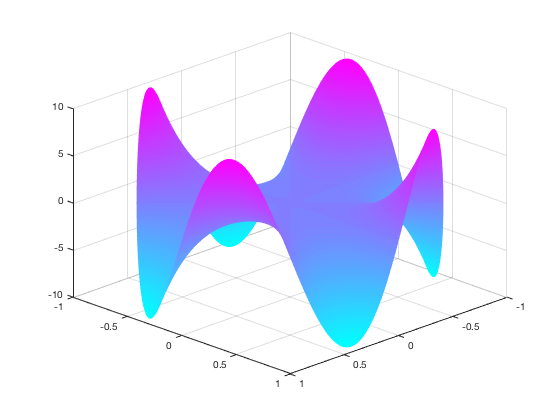
\includegraphics[width=5cm]{images/swing_function_plot.png}
%   \caption{$u(x)$}%{Numerically solved solution}
%   \label{fig:swingPlot}
% \end{figure}


% Equations can also be labeled
% \begin{equation}
% 	\pi = \mathrm{e}^{i\cdot\phi}
% 	\label{eq:equation1}
% \end{equation}


% And later referenced. Even in subfigures.
% \begin{figure}[!htb]
%   \centering
%   \begin{subfigure}[b]{0.3\textwidth}
%     \centering
%   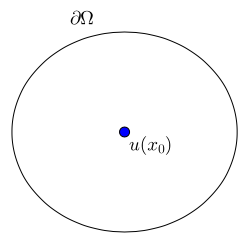
\includegraphics[width=\textwidth]{images/CircCenter}
%   \caption{Equation~\ref{eq:equation1}}\label{fig:circcenter}
% \end{subfigure}
% \hfill
%   \begin{subfigure}[b]{0.3\textwidth}
%     \centering
%   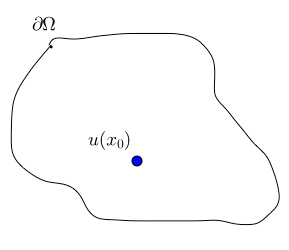
\includegraphics[width=\textwidth]{images/GeneralOffset}
%   \label{fig:generaloffset}
%   \caption{Equation~\ref{eq:equation1}}
% \end{subfigure}
% \end{figure}
% \section{Including code}

% Code can be using the package
% \href{https://www.sharelatex.com/learn/Code\_Highlighting\_with\_minted}{Minted}.

% An exaple of which of can be found below (see Source Code~\ref{lst:nice_listing})
% \begin{listing}
% 	%the language syntax can be declared here.
% 	\begin{minted}{python} 
% 	import numpy as np
	
% 	def incmatrix(genl1,genl2):
% 	    m = len(genl1)
% 	    n = len(genl2)
% 	    M = None #to become the incidence matrix
% 	    VT = np.zeros((n*m,1), int)  #dummy variable
	
% 	    #compute the bitwise xor matrix
% 	    M1 = bitxormatrix(genl1)
% 	    M2 = np.triu(bitxormatrix(genl2),1)
	
% 	    for i in range(m-1):
% 	        for j in range(i+1, m):
% 	            [r,c] = np.where(M2 == M1[i,j])
% 	            for k in range(len(r)):
% 	                VT[(i)*n + r[k]] = 1;
% 	                VT[(i)*n + c[k]] = 1;
% 	                VT[(j)*n + r[k]] = 1;
% 	                VT[(j)*n + c[k]] = 1;
	
% 	                if M is None:
% 	                    M = np.copy(VT)
% 	                else:
% 	                    M = np.concatenate((M, VT), 1)
	
% 	                VT = np.zeros((n*m,1), int)
	
% 	    return M
% 	\end{minted}

%   \caption{My nice listing}
%   \label{lst:nice_listing}
% \end{listing}
Fluid mechanics plays a pivotal role in the progress of various diverse fields, including aerospace and automotive engineering, energy system optimization, environmental modeling, biomedical research, and countless other critical domains that shape our technological and scientific landscape. Partial Differential Equations (PDEs), in particular the Navier-Stokes equations, which provide the mathematical framework for analyzing the behaviour of fluid flow for these complex problems are often intractable, i.e; they do not have exact analytical solutions. Thus, they still remain an open problem in the world of mathematics. Hence, the solutions to the Navier-Stokes equations are approximated using numerical methods such as the Finite Element or the more commonly used Finite Volume Method (FVM) which rely on spatial and temporal discretization of PDEs. With the advent of software and technology, emerged the field of Computational Fluid Dynamics (CFD), leveraging computer algorithms for numerical simulations of fluid flow problems. However, these simulations are computationally intensive and may take from several hours to several weeks for complex flows and/or geometries. Although advances in high-performance computing and parallel processing have been a game-changer for CFD, there still remain several complications with respect to grid dependency, convergence issues, model assumptions and simplification of underlying physics, numerical errors as well as turbulence modelling. \\
The most problematic use-case is turbulence modelling, which is marked by velocity and pressure fluctuations, a wide range of length and time scales - from large vortices down to small eddies and numerical instabilities. In addition, modelling turbulence near walls presents unique problems on its own which requires specialized treatments and techniques in these near-wall regions. Accurately modelling all the intricate phenomena of the turbulent regime, called the Direct Numerical Simulation (DNS), is possible, but at the cost of a huge amount of computational resources, complexity and simultaion times. Consequently, in many practical scenarios, simplified turbulence models are employed, even though this comes at the expense of accuracy. \\
Advancements in the dynamic field of CFD over the past had seen substantial efforts channeled into enhancing turbulence models, improving meshing techniques, efficient Reduced Ordered Modelling (ROM) surrogates and reducing computational complexity. While numerous techniques and models exist to address various turbulence-related challenges, there is no universally applicable model that consistently delivers accurate results across all turbulence settings. As a result, the computational bottleneck often remains an unavoidable obstacle. In response to this challenge, in recent times, there has been a growing interest in implementing Machine Learning (ML) algorithms, specifically to enhance the cost-effectiveness of CFD methods. Although training an ML model is often very computationally demanding, a trained model can quickly make predictions on new data, a significant advantage over the commonly used numerical methods. The integration of ML in CFD represents a paradigm shift, enabling simulations to move beyond traditional physics-based models. The synergy between Deep Learning (DL) and CFD offers the potential to uncover novel insights into fluid dynamics, for example, Convolutional Neural Networks (CNNs) can extract relevant features and classify flow regimes whereas Recurrent Neural Networks (RNNs) can predict fluid behaviors based on temporal data for unsteady flows. Incorporating neural networks into fluid dynamics problems not only improves the accuracy and efficiency of simulations, but also opens up new doors for understanding flow behaviours and strategies for flow control and optimization. As neural networks continue to evolve and adapt to the specific challenges of fluid dynamics, they promise to be a pivotal component in the advancement of CFD across various industries and applications. \\
So far, ML methods have been employed in fluid dynamics research but have not been in engineering practice. Some possible explanations for this might be the scarcity of huge datasets that are open and can be publicly accessed and the poor generalization performance of ML techniques on previously unseen data. This thesis attempts to tackle the generalization problem by implementing a novel approach that combines GNNs with a meta learning principle for accurate and efficient predictions even on unencountered datasets. 
\section{Literature Review}
In this section, relevant research and work done with respect to ML in the context of CFD, especially in turbulence modelling is discussed. The evolution of turbulence modeling is a dynamic field with notable milestones and contributions. The pioneering work of Osborne Reynolds in the late 19th century laid the foundation for turbulence research, leading to the eddy viscosity hypothesis and the rise of Reynolds-averaged Navier-Stokes (RANS) modeling in the mid-20th century. The K-epsilon model, introduced in the 1970s, significantly enhanced RANS modeling by striking a balance between accuracy and computational efficiency. Parallel to this development, Large Eddy Simulation (LES) emerged as a complementary approach, aiming to capture large-scale turbulent eddies directly while modeling smaller ones. Advances in computational power enabled the feasibility of LES, particularly for complex geometries and higher Reynolds numbers. Direct Numerical Simulation (DNS), which resolves all turbulent scales, became increasingly attainable due to further advancements in computational resources. Recent research has focused on improving existing models, developing advanced closure schemes, and exploring the use of machine learning techniques. The combination of RANS and LES techniques in hybrid models has also gained traction, offering a promising path towards more efficient and accurate simulations. \\


%% ---------------------------------------------------------------------------
%%
%% Thesis content: What did you do?
%%
%%% ---------------------------------------------------------------------------
\part[Theory]{Background Theory - Fluid Dynamics and Deep Learning}
\label{part:Theory}
\chapter{Nozzle simulation and fluid mechanics primer}
\label{chap:Theory-CFD}
This chapter delves into the nozzle flow dynamics of a High-speed Orienting Momentum with Enhanced Reversibility (HOMER) nozzle, as developed by Trancossi and Dumas \cite{trandum}. We begin with an understanding of the problem and the underlying principle, which is the Coanda effect. In Section \ref{goveq}, we elucidate the governing equations that mathematically define the fluid flow, as well as additional equations for turbulence modelling. Subsequently, we discuss various numerical approaches that discretize the governing equations. Additionally, the chapter provides insights into the simulation setup in Section \ref{setup}, encompassing meshing strategies, boundary condition specifications, and solver settings for the problem. 
\section{Jet deflection in the HOMER nozzle}  
The HOMER nozzle is designed to produce a controllable and selective deviation of a synthetic jet, generated by mixing two primitive jets, without requiring any mechanical part but solely by taking advantage of the Coanda effect. The general structure of the nozzle is depicted in Figure \ref{fig:nozzle}. As we can see from the figure, the nozzle has two inlets fed by two impinging jets, followed by a convergence zone, or a septum, where mixing of the flows occurs. The mixing of flows generates a synthetic outflow jet, which can be controlled by modifying the momentums of the primitive jets. Next to the convergence zone is the outflow mouth, with curved walls connected to two convex Coanda surfaces on the top and bottom.
\begin{figure}[ht]
  \centering
  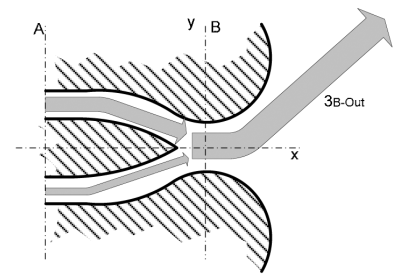
\includegraphics[width=8cm]{images/Theory-CFD/nozzle2.png}
  \caption{Schematic Overview of the HOMER Nozzle Design: Highlighting dual inlets and Coanda effect surfaces, adapted from Trancossi and Dumas \cite{trandum}}
  \label{fig:nozzle}
\end{figure}
The system requires a minimum operating condition of the primitive jets to ensure effective mixing (\cite{trandum}). The impinging jets must have velocities high enough to generate a synthetic jet of Reynolds number greater than 5000 at the outlet mouth. To guarantee optimum operation, the Reynolds number at the outlet must exceed 10000. In the case of lower Reynolds numbers, the system's behavior is unpredictable. 
\subsection{Coanda effect}
Coanda effect is the tendency of a stream of fluid emerging from an orifice to follow an adjacent flat or a curved surface and to entrain fluid from the surroundings so that a region of lower pressure develops. In simple terms, it is the tendency of a fluid to adhere to and stay attached to the walls of a convex surface, as demonstrated in Figure \ref{fig:Coanda}. Different fluid dynamic effects concur to create the Coanda effect, namely the boundary layer effect, the adhesion effect, and the attraction effect. Newman \cite{newman} has demonstrated that Coanda adhesion to a curved surface is dependent on the equilibrium of forces applied on the fluid. Adhesive motion on a curved surface involves centrifugal force and radial pressure, with contact pressure decreasing due to viscous drag upon jet exit. This pressure differential propels fluid along the curved surface until surface pressure matches ambient pressure, causing detachment between the wall and the fluid jet. 
\begin{figure}[ht]
    \centering
    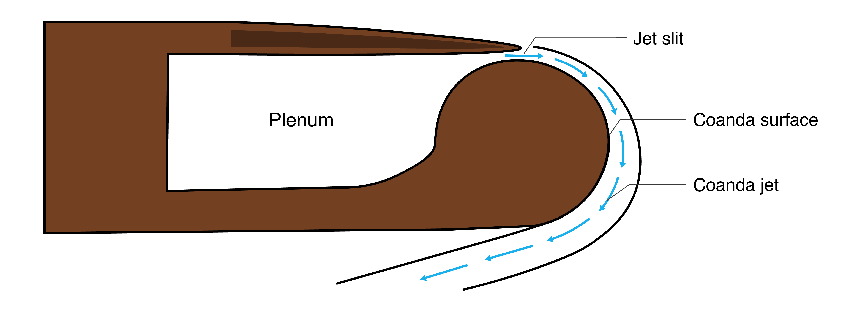
\includegraphics[width=10cm]{images/Theory-CFD/Coanda-effect.png}
    % \caption{Concept of Coanda effect: A fluid jet emerging from the orifice tends to adhere to the adjacent curved surface.}
    \caption{Demonstration of the Coanda Effect: Visualization of a fluid jet adhering to and flowing along a curved surface, illustrating the fundamental principle utilized in the HOMER nozzle design.}
    \label{fig:Coanda}
  \end{figure}
% \section{Flow Simulation}
\section{Governing equations} \label{goveq}
In this section, we talk about the mathematical equations that govern the fluid flow in the nozzle setup. The Navier-Stokes equations (NSE) can be used to mathematically model the flow of an incompressible, Newtonian fluid within the computational domain. Figure \ref{fig:Domain} shows the computational domain for our fluid flow problem. We consider the same homogenous fluid for both primitive jets. This refers to streams with the same chemical and physical properties, i.e; the density of the fluid $\rho$ remains constant. The fluid in consideration is air in ideal gas conditions. 
\begin{figure}[ht]
  \centering
  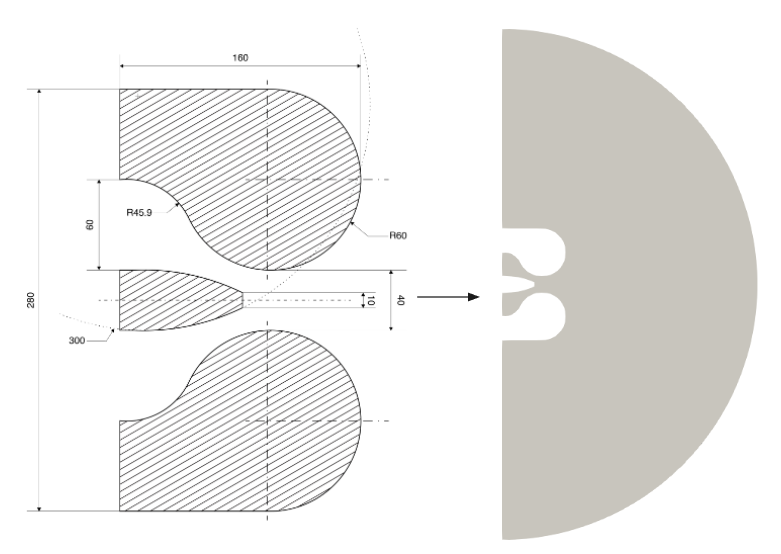
\includegraphics[width=12cm]{images/Theory-CFD/Flow Domain.png}
  \caption{Visualization of the HOMER Nozzle: Left - Geometry of the modified HOMER nozzle; Right - CAD model showcasing the computational simulation domain.}
  \label{fig:Domain}
\end{figure}
\begin{equation}
  \begin{aligned}
  \frac{\partial u_i}{\partial x_i}&=0\\
  \frac{\partial u_i}{\partial t}+u_j \frac{\partial u_i}{\partial x_j}&=\frac{-1}{\rho} \frac{\partial p}{\partial x_i}+\nu \frac{\partial^2 u_i}{\partial x_j^2}
  \end{aligned}
  \end{equation}
where, $u_i$ is the flow velocity in the spatial direction $x_i$, $\nu$ is the kinematic viscosity, $\mu$ is the dynamic viscosity ($\nu = \mu / \rho$), $p$ is the pressure. A velocity profile from a fully-developed turbulent plane channel flow is prescribed as inlet velocities at $\partial{\Omega_{in}}$. At the walls $\partial{\Omega_{wall}}$, we apply no-slip boundary conditions. We impose zero-gradient Neumann boundary conditions on the flow quantities at the outlet.\\
Turbulence, characterized by its unsteady, highly irregular, rotational and energy dissipative behaviors at high Reynolds numbers, causes minute fluctuations in velocity, pressure, and temperature across varying scales. While a direct numerical solution (DNS) could theoretically capture these fluctuations by solving the NSE, the immense computational resources required render it impractical for most engineering simulations. 
% Turbulence modelling serves as a pragmatic approach to predict time-averaged fields without needing to resolve every turbulent detail.
Turbulence modelling using RANS (Reynolds-Averaged Navier-Stokes) equations offers a practical compromise by solving time-averaged equations for steady-state or unsteady (URANS) flows. RANS relies on turbulence models to account for unresolved turbulence effects, allowing for efficient simulations of complex engineering systems without resolving every turbulent detail. The underlying principle is to consider the flow as the sum of the mean flow and turbulent/fluctuating components. For a steady-state flow field, Reynolds decomposition is applied to flow quantities. For example, the flow velocity is expressed as $u_i = U_i + u_i^{\prime}$, where $U_i$ is the mean velocity and $u_i^{\prime}$ is the fluctuating turbulent component. The Reynolds averaging process introduces an additional term to the NSE known as Reynolds stress. By substituting the averaged quantities in the NSE, we obtain the RANS equations for our steady-state, 2D incompressible flow as,
\begin{equation}
  \begin{aligned}
  \frac{\partial u_i}{\partial x_i}&=0 \\
  u_j \frac{\partial u_i}{\partial x_j}&=\frac{1}{\rho}\frac{\partial}{\partial x_j}     \left[-p \delta_{i j}+\mu \left(\frac{\partial u_i}{\partial x_j}+\frac{\partial u_j}{\partial x_i}\right) - \rho u'_i u'_j \right]
  \end{aligned}
\end{equation}
where $- \rho u_i^{\prime} u_j^{\prime}$ is called the Reynolds stress tensor and represents the effect of the small-scale turbulence on the average flow. Here, $u$ and $P$ are the averaged flow quantities $\langle u \rangle $ and $\langle P \rangle $ but the averaged notation $\langle ... \rangle $ has been omitted for convenience. The RANS equations have no unique solution because they are not in closed form, the unknowns being more than the equations. Thus, additional equations are needed for turbulence closure. The most common strategy used in CFD is to relate the Reynolds stress to the shear rate by the Boussinesq relationship:
\begin{equation}
  u_i^{\prime} u_j^{\prime}=2 \frac{\mu_t}{\rho} S_{i j} \quad \text { with } \quad S_{i j}=\frac{1}{2}\left(U_{i, j}+U_{j, i}\right)
\end{equation}
where $\mu_t$ is the turbulent viscosity, which is usually computed from the turbulence models. Some of the RANS-based turbulence models are outlined below: 
\begin{enumerate}
  \item The Spalart-Allmaras model is a one-equation model that is computationally efficient. It solves for a single variable, the turbulent viscosity, using a transport equation derived from the RANS equations. 
  % This model is particularly suited for aerodynamic flows, offering reliable predictions with reduced computational cost.
  \item The $\text{k}-\epsilon$ model resolves turbulence through two transport equations: one for turbulent kinetic energy ($\text{k}$) and another for the rate of dissipation of turbulent kinetic energy ($\epsilon$). 
  % These equations govern the behavior of turbulence in a wide range of flows, from boundary layers to free shear flows.
  \item The $\text{k}-\omega$ model is another two-equation turbulence model that features transport equations for turbulent kinetic energy and a specific rate of turbulence dissipation ($\omega$). This model is particularly advantageous in accurately predicting near-wall flows and is less susceptible to numerical issues than the $\text{k}-\epsilon$ model in adverse pressure gradient regions. 
  \item The $\text{k}-\omega$  SST (Shear-Stress Transport) model combines aspects of the $\text{k}-\epsilon$ model near walls and the $\text{k}-\omega$ model away from walls to provide accurate predictions in both regions. The $\text{k}-\omega$ SST model is particularly suitable for boundary layer flows, capturing the near-wall behavior accurately while providing robust predictions in the outer flow regions. Its versatility and computational efficiency make it a popular choice for a wide range of engineering applications.
\end{enumerate}
For the purposes of this work, the $\text{k}-\omega$ SST turbulence model has been adopted.
\section{Numerical analysis}
Numerical analysis on PDEs - in our case, the RANS equations is performed by discretizing the continuous domain into a discrete setup, which results in a system of algebraic equations which are usually linear systems that can be solved by iterative techniques such as Jacobi or Gauss-Seidel. Multigrid methods are another class of iterative numerical techniques used to solve discretized PDEs efficiently for large-scale computational problems. They employ a hierarchy of grids with varying levels of resolution, combining coarse and fine grids to accelerate convergence. By addressing error components on multiple scales, multigrid methods effectively smooth out high-frequency errors while retaining accuracy, making them suitable for problems with smooth solutions or complex geometries. \\
Some commonly used discretization techniques are the Finite Difference Method (FDM), Finite Element Method (FEM), and Finite Volume Method (FVM). All three methods end up solving one (or several) system(s) of linear equations to compute an approximate numerical solution of the PDE at hand. And for all three methods, these linear systems are sparse, and the equation for an unknown $u_i$ involves only a few neighbors of point $i$. Overall, FDM is mostly used for geometries that can be discretized by structured grids (e.g., rectangles), while FEM and FVM are more suitable for complex domains. \\
FVM discretizes PDEs by dividing the computational domain into finite volumes or cells. It conservatively approximates integral forms of conservation laws within each cell. The method calculates fluxes across cell interfaces, preserving conservation principles, making it particularly suited for problems involving fluid flow, heat transfer, and other conservation phenomena. As FVM is based on the integral formulation of a conservation law, it is mainly used to solve PDEs in fluid dynamics, which involves fluxes of the conserved variable. In this thesis, we are only interested in the discretization of PDEs using FVM, which is the most widely used discretization approach in CFD solvers. 
% In the case of non-linear systems arising from discretization, linearization schemes are required to convert the non-linearity into a sequence of linear systems: a sequence of linearized equations is solved iteratively, converging to the solution of the non-linear system. 
\section{Simulation setup} \label{setup}
Trancossi and Dumas \cite{trandum} proposed a mathematical model of the HOMER nozzle and carried out 2D, incompressible flow simulations on this geometry. The simplified model predicts the detachment angle of the jet stream over the curved surface. The nozzle chosen for our study is a slightly modified version of a thrust-vectoring propulsive HOMER nozzle. The modified design is inspired by the numerical investigation and experimental validation of Kara and Erpulat \cite{kara}. The geometry adopted for the simulations as well as the computational domain are depicted in Figure \ref{fig:Domain}. The selected channel length ensures the mean flow quantities are fully-developed, hence establishing steady-state conditions. The meshing and CFD simulation are carried out on \verb|OpenFOAM| which uses finite volume methods to discretize the PDEs. 
\subsection{Mesh generation}
The geometry is created using FreeCAD \cite{FreeCAD} and patch names are assigned based on the type of boundaries.  The meshing process on \verb|OpenFOAM| begins with the discretization of the geometry into hexahedral blocks using \verb|blockMesh|. Then, \verb|snappyHexMesh| refines the mesh based on parameters specified in \verb|snappyHexMeshDict|. This includes defining refinement controls, snapping settings, adding boundary layers, and ensuring mesh quality. The process iteratively refines the mesh until the desired quality and resolution are achieved, enabling accurate simulations of the geometry's physical behavior. An unstructured, 3D hybrid mesh with tetrahedral and hexahedral elements mesh has been generated for the computational domain and is enhanced by boundary layer refinement and a refinement box around the nozzle region.
\subsection{Boundary conditions and solver settings}
% An incompressible steady-state CFD simulation is carried out on the mesh by setting appropriate boundary and initial conditions. For $k$, \( \omega \) and turbulent viscosity $\nu_t$, low Reynolds number wall functions are applied at walls to account for near-wall turbulence effects. This ensures accurate modeling of turbulence near boundaries. Pressure is set to zero gradient at the walls to maintain a neutral pressure condition. Adiabatic stationary walls with no slip conditions are prescribed at the Coanda surfaces as well as the inner walls of the nozzle. Inlets are prescribed with fixed values of velocities to define the flow entering the domain. Both the inlet turbulence intensities are set to 1\% (medium turbulence). Additionally, a pressure outlet boundary condition is used to specify the pressure at outlets, allowing flow to exit the domain without reflecting back. These boundary conditions collectively ensure proper representation of the flow behavior within the computational domain. The simulations are performed using the \verb|simpleFoam| solver which utilizes the SIMPLE (Semi-Implicit Method for Pressure Linked Equations) algorithm for pressure-velocity coupling. This method iteratively resolves the momentum and pressure equations until a predetermined convergence criterion is satisfied. The $k-\omega$ SST turbulence model is utilized, and the kinematic viscosity of the fluid is taken as $1.51e^{-5}$. The convective term of velocity is discretized using the linear UpwindV scheme whereas the divergence term of velocity is discretized using a bounded Gauss linear scheme. For the discretization of the divergence of the turbulence fields $k$, $\omega$, $\nu_t$, a bounded Gauss upwind scheme is used. In this case, the convergence criterion was set to $10e^{-6}$ for the pressure field and $10e^{-8}$ for all other quantities. 
We carry out an incompressible steady-state CFD simulation on the mesh, setting appropriate boundary and initial conditions. By applying low Reynolds number wall functions for $k$, \( \omega \), and turbulent viscosity $\nu_t$ at walls, we account for near-wall turbulence effects, ensuring accurate modeling near boundaries. To maintain a neutral pressure condition, we set the pressure to zero gradient at the walls. We also prescribe adiabatic stationary walls with no slip conditions at the Coanda surfaces and the inner walls of the nozzle. We define the flow entering the domain by prescribing inlets with fixed velocities and set both inlet turbulence intensities to 1\% (medium turbulence). Furthermore, we specify the pressure at outlets through a pressure outlet boundary condition, allowing flow to exit the domain without reflecting back. These actions collectively ensure the proper representation of flow behavior within the computational domain. The \verb|simpleFoam| solver is the tool we use for the simulations, employing the SIMPLE (Semi-Implicit Method for Pressure Linked Equations) algorithm for effective pressure-velocity coupling. We iteratively resolve the momentum and pressure equations until achieving a predetermined convergence criterion. The $k-\omega$ SST turbulence model serves our purposes, with the fluid's kinematic viscosity set at $1.51e^{-5}$. For velocity's convective term, we use the linear Upwind scheme for discretization, while the divergence term undergoes discretization via a bounded Gauss linear scheme. For the turbulence fields $k$, $\omega$, $\nu_T$, we employ a bounded Gauss upwind scheme for discretization. We have set the convergence criterion to $10e^{-6}$ for the pressure field and $10e^{-8}$ for all other quantities.


\chapter{Deep learning primer}
\label{chap:Theory-Deep Learning}
This chapter provides a comprehensive explanation of foundational concepts and methodologies in deep learning, with a particular emphasis on Graph Neural Networks (GNNs). It begins by introducing deep learning and elucidating the basics of neural networks, focusing on their architecture and operational principles. Section \ref{optrain} navigates through the intricacies of training neural networks with topics including data partitioning, feature scaling, weights initialization, regularization, batch training, and hyperparameter tuning. Subsequently, it delves into optimization techniques, addressing essential elements such as loss functions, backpropagation, learning rates, and optimizers. Furthermore, this chapter examines model evaluation metrics and explores advanced neural network architectures such as CNNs in Section \ref{cnnse} and GNNs in Section \ref{gnnse}, highlighting their important features and components. 

\section{Introduction to machine learning and deep learning}
Machine learning, a dynamic subset of artificial intelligence, is dedicated to developing algorithms that extract insights and patterns from data. This enables systems to enhance their accuracy and decision-making capabilities without being explicitly programmed for each task. The learning process utilizes statistical models and optimization algorithms to iteratively adjust parameters and improve performance. Machine learning approaches are broadly categorized into supervised learning and unsupervised learning based on learning objectives. \\

\textbf{Supervised learning} involves training a model using labeled data, where each input is paired with a corresponding output. During training, the model learns to map input data to output labels by minimizing the difference between its predictions and the true labels. This approach is commonly used for tasks such as classification and regression. \\

\textbf{Unsupervised learning}, involves training a model on unlabeled data, where the algorithm aims to find hidden patterns or structures within the data without explicit guidance. Unsupervised learning is often used for tasks like anomaly detection, data exploration, and feature learning, where the data lacks labeled examples or where the underlying structure is unknown. \\

Deep learning is a subset of machine learning that has gained significant attention due to its remarkable performance in various tasks, ranging from image and speech recognition to autonomous driving. It utilizes neural networks consisting of multiple layers of interconnected neurons to learn representations of data through iterative processing of input data to make predictions or decisions. Henceforth, when we mention machine learning or deep learning, it refers to supervised learning in this context, unless otherwise specified.
\section{Fundamentals of neural networks}
\gls{ANN} are computational models inspired by the structure and function of biological neural networks \cite{rumel}. They consist of interconnected nodes organized into layers, typically including an input layer, one or more hidden layers, and an output layer. \\ 
A \textbf{perceptron} or an artificial neuron, is the fundamental building block of ANNs. It takes multiple input signals $\mathbf{x}= \left(x_1, x_2 ...x_n\right)$, each weighted by a connection weight $w_1,w_2,...w_n$, sums them up, and applies an activation function $\sigma$ to produce an output $\mathbf{y} = \sigma \left(\mathbf{w}^T\mathbf{x} + \mathbf{b} \right)$, where $\mathbf{b}$ is the bias. Perceptrons are arranged in layers to build complex neural network architectures.\\
\begin{figure}[ht]
    \centering
    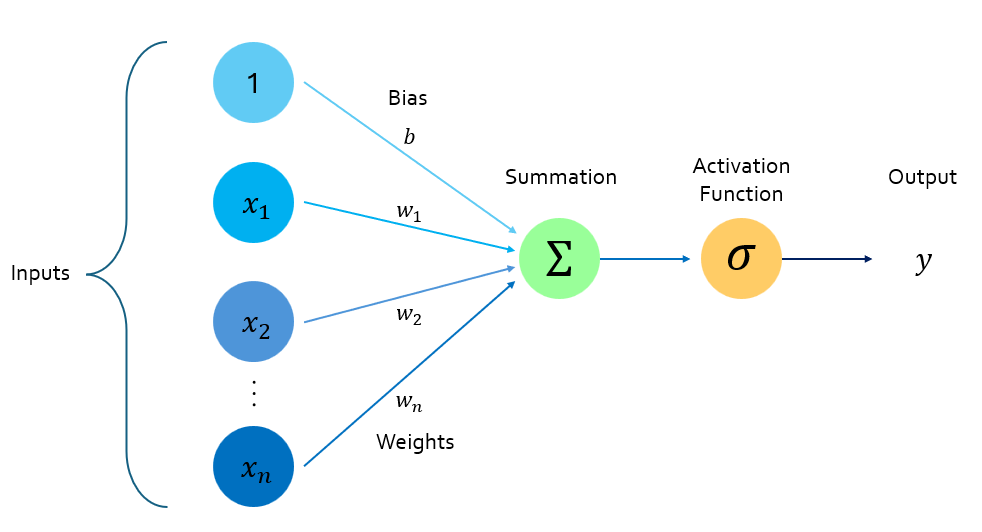
\includegraphics[width=12cm]{images/Theory-DL/ActFn.png}
    \caption{Schematic representation of a perceptron - the basic computational unit of artificial neural networks, illustrating input connections, weights, bias, and an activation function.}
    \label{fig:Perceptron}
  \end{figure}
\textbf{Activation functions} are usually non-linear functions to introduce non-linearity within the layers of neural networks, allowing them to learn and represent complex relationships in data. Common activation functions include sigmoid, tanh, \gls{ReLU}, and leaky ReLU. Activation functions transform the weighted sum of inputs $\mathbf{z}$ into the output signal $\mathbf{y}$, typically in the range between 0 and 1 (for sigmoid) or -1 and 1 (for tanh). Without the nonlinear transformation via the activation function, the network would be confined to solving merely linear problems. \\
\begin{figure}[ht]
    \centering
    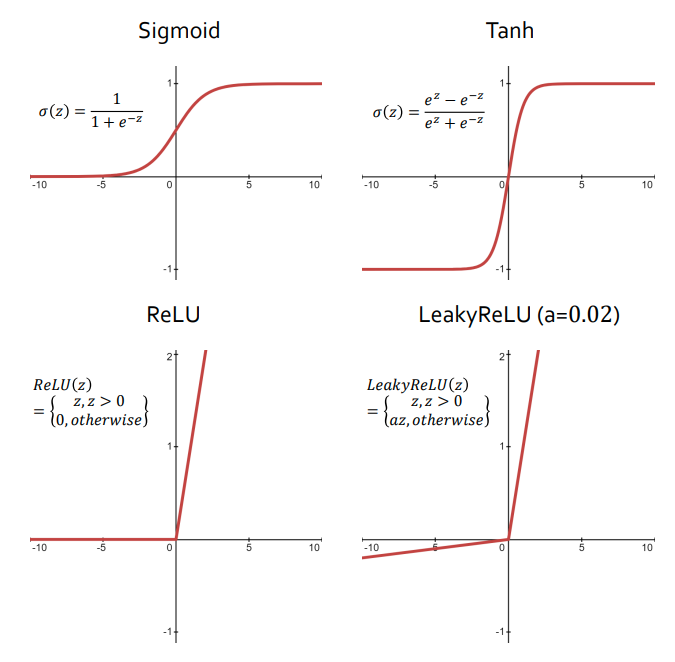
\includegraphics[width=8cm]{images/Theory-DL/ActGraphs.png}
    \caption{Comparative visualization of common activation functions used in neural networks: (a) Sigmoid, (b) Tanh, (c) ReLU, and (d) Leaky ReLU.}
    \label{fig:ActGraphs}
  \end{figure}
\textbf{Weights} in a neural network represent the strength of connections between neurons. They are learned parameters to adjust the influence of input signals on the neuron's output. \textbf{Biases} allow neural networks to model the offset from zero output, influencing the activation of neurons regardless of the input.\\
\textbf{Neural networks} consist of interconnected layers of perceptrons that process input data to produce output predictions. \gls{NN} can be represented as directed graphs, where nodes correspond to perceptrons, and edges depict connections between them. These connections typically carry weighted signals from one neuron's output to another neuron's input. In particular, we are interested in \textbf{feed-forward neural networks}, in which, information flows only in one direction, from the input layer through one or more hidden layers to the output layer. Each layer processes the input data independently, and the output of one layer serves as the input to the next layer. The connections between neurons do not form directed cycles, ensuring that the network architecture is acyclic. \gls{MLP} are the simplest feed-forward neural networks, and their architecture is described in Figure \ref{fig:MLP}. 
\begin{figure}[ht]
    \centering
    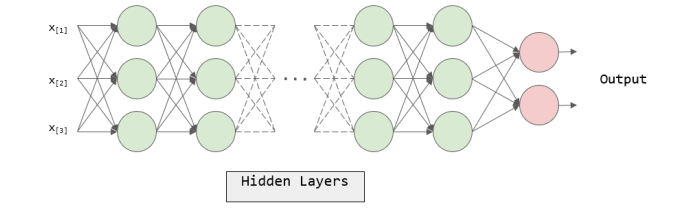
\includegraphics[width=10cm]{images/Theory-DL/MLP.png}
    \caption{Architecture of a Multi-Layer Perceptron (MLP) showcasing an input layer, multiple hidden layers, and an output layer, demonstrating the flow of information in feed-forward neural networks.}
    \label{fig:MLP}
  \end{figure}
\section{Training of neural networks}\label{optrain}
In this section, we delve into the training practices of neural networks, highlighting the optimization of model parameters to enhance task performance. We particularly focus on the methodologies for data handling like data partitioning, feature scaling, and regularization techniques that address model generalization as well as batch training and weight initialization.
% , critical for achieving predictive accuracy across diverse datasets.
The process of training neural networks is fundamentally aimed at optimizing a model's parameters to improve its performance on given tasks. Thus, we also talk about optimization strategies, which leverage algorithms like backpropagation to calculate gradients and apply updates via optimizers such as SGD or Adam.
\subsection{Data partitioning}Data partitioning is a crucial step in deep learning in which the dataset is divided into separate subsets for training, validation, and testing. The data partitioned into training data is used to train the model, and validation data is used to tune hyperparameters and monitor performance. The testing data is used to evaluate the final model's generalization performance. The partitioning process ensures that the model's performance is assessed accurately on unseen data and provides independent datasets for training and evaluation. 
\subsection{Feature scaling}Feature scaling or normalization, is a preprocessing step aimed at bringing all input features to a similar scale. Features with large magnitudes can lead to large gradients during training, which may cause unstable behavior and make it challenging for the optimizer to find the optimum. Feature scaling mitigates this issue by reducing the range of feature values, thus preventing gradient instability and ensuring more reliable optimization. Common feature scaling techniques include,
\begin{enumerate}
\item Min-Max normalization: $x^{\prime}=\frac{x-x_{\min }}{x_{\max }-x_{\min }}$
\item Z-Score standardization: $x^{\prime}=\frac{x-\tilde{x}}{\sigma}$
\item Unit length scaling: $\mathrm{x}^{\prime}=\frac{\mathrm{x}}{\|\mathrm{x}\|}$
\end{enumerate}
\subsection{Weight initialization}
Weight initialization sets the initial values for the model's parameters before training begins. The loss landscape of deep neural networks is complex and non-convex, with multiple local minima. The initial weights dictate the local minimum the weights should converge to; thus, better initialization leads to improved model performance. There are different cases to consider for weight initialization: 
\begin{enumerate}
\item Initializing all weights to 0 or a constant leads to symmetrical gradients and weight updates across all neurons in the network during backpropagation. This results in the neurons learning identical features, causing the network to lose its representational capacity.
\item Large weights can lead to exploding gradients during training. Large weights can saturate activation functions, pushing them into regions of zero gradients (e.g., in sigmoid or tanh activations), hindering learning and resulting in slow convergence.
\item Small weights help prevent exploding gradients, as activations and gradients remain within a manageable range during training. However, extremely small weights results in small activations, leading to vanishing gradients. 
\end{enumerate}
% In summary, weight initialization is crucial for initializing neural networks effectively. 
Random initialization with small weights is a common practice in deep learning. Initializing weights to random values drawn from a suitable distribution with a zero mean and small variance breaks symmetry and helps prevent both vanishing and exploding gradients. It encourages each neuron to learn different features from the input data, promoting diverse representations and effective learning. Techniques like Xavier and Kaiming initialization further refine this process by adapting to the specific characteristics of activation functions.
\subsubsection{Xavier-Glorot initialization}
This technique \cite{glorot} initializes weights from a normal or uniform distribution with a zero mean. The variance of the distribution is adjusted based on the number of input neurons (fan-in) and output neurons (fan-out) as $\text{Var}(W) = \frac{2}{\text{fan}_{\text{in}} + \text{fan}_{\text{out}}}$. Xavier initialization is commonly used in shallow networks with symmetric activation functions, ensuring balanced weight initialization and stable training dynamics. 
\subsubsection{Kaiming-He initialization}
Kaiming initialization \cite{he2015} is designed for networks using non-linear activations like ReLU as seen in modern deep learning architectures. It initializes weights from a normal distribution with zero mean, adjusting the variance based on fan-in as $ \text{Var}(W) = \frac{2}{\text{fan}_{\text{in}}}$. Kaiming initialization helps mitigate the issue of vanishing gradients associated with \gls{ReLU} activations, ensuring stable training and faster convergence.
\subsection{Regularization}
Regularization broadly refers to techniques used to prevent overfitting by imposing additional constraints on the model's parameters, i.e; by adding penalties to the loss function, thus discouraging complex models. Regularization penalizes large weights in the model, thereby promoting simpler models that generalize better to unseen data. Two common forms of regularization are L$_2$ regularization (Lasso) and L$_1$ regularization (Ridge). \\
L$_1$ regularization encourages sparsity in the weights, performing feature selection by setting irrelevant weights to zero, making the model simpler and more interpretable. 
\[ \operatorname{Loss}_{\mathrm{L}_1}=\operatorname{Loss}_{\text {original }}+\lambda \sum_{i=1}^n\left|w_i\right| \]
L$_2$ regularization encourages the weights to be spread out more evenly, preventing individual weights from becoming too large.
\[ \operatorname{Loss}_{\mathrm{L}_2}=\operatorname{Loss}_{\text {original }}+\lambda \sum_{i=1}^n w^2_i \]
Here, $\lambda$ is the regularization strength and determines the degree of penalty imposed on large weights. A smaller $\lambda$ value results in weaker regularization, allowing the model to fit the training data more closely but increasing the risk of overfitting. Conversely, a larger $\lambda$ value increases the regularization effect, resulting in a simpler model that generalizes better but may underfit the training data if set too high.
\subsubsection{Dropout}
Dropout is a regularization technique used in neural networks during training, where a random fraction of neurons is temporarily dropped out or ignored during forward and backward propagation. This prevents neurons from co-adapting and overfitting to the training data, promoting robustness and generalization. 
\subsection{Batch training and batch normalization}
Batch training is a technique in deep learning in which the model updates its parameters based on a subset (or batch) of the training data, rather than the entire dataset. The training data is divided into batches of fixed size, and the model computes the loss gradients for each batch using backpropagation. Since it computes the gradient updates based on an average over the samples in each batch, this reduces the variance in the gradient estimates compared to processing the entire dataset at once. This averaging effect stabilizes the gradients and prevents large fluctuations during training. \\
Selecting an appropriate batch size is crucial, as too small a batch size leads to frequent updates and noisy gradient updates. On the other hand, too large a batch requires more computational resources and memory despite providing precise gradient estimates, leading to stable optimization and faster convergence. Optimal batch size requires balancing the trade-off between computational efficiency and the quality of gradient estimates. \\                     
Another important term in this context is an epoch, which refers to a single pass through the entire training dataset. During one epoch, each batch is processed sequentially through the neural network. Once all batches have been processed, completing a full iteration over the entire dataset, one epoch is considered complete. Typically, training iterates over the entire dataset for multiple times or epochs until the model converges or a predefined stopping criterion is met. \\
% Batch normalization (BatchNorm) is another technique used in deep learning to stabilize and accelerate training by normalizing the activations of each layer within a mini-batch. 
Batch normalization \cite{batchnorm} is a technique to improve the stability of neural networks by normalizing the activations of each layer. It operates on mini-batches of data and normalizes the input of each layer to have a mean of zero and a standard deviation of one. This is achieved by computing the mean and standard deviation of the activations across the batch, and then scaling and shifting the activations using learned parameters. The batch normalization transformation for a layer with input $x^{(1)}, x^{(2)}, \ldots, x^{(m)}$ is given as,
\begin{equation}
\begin{aligned}
& \mu_B=\frac{1}{m} \sum_{i=1}^m x^{(i)} \\
& \sigma_B^2=\frac{1}{m} \sum_{i=1}^m\left(x^{(i)}-\mu_B\right)^2 \\
& \hat{x}^{(i)}=\frac{x^{(i)}-\mu_B}{\sqrt{\sigma_B^2+\epsilon}} \\
& y^{(i)}=\gamma \hat{x}^{(i)}+\beta
\end{aligned}
\end{equation}
where $\mu_B$ and $\sigma_B^2$ are the mean and variance of the mini-batch $B$ of size $m$, $\epsilon$ is a small constant added to avoid division by zero, $\hat{x}^{(i)}$ is the normalized input, $\gamma$ and $\beta$ are learnable parameters (scale and shift), and $y^{(i)}$ is the output of the batch normalization layer.
\subsection{Overfitting and underfitting}
Overfitting and underfitting are two common phenomena that affect the performance and generalization ability of the model. Overfitting occurs when a model learns to perform well on the training data but fails to generalize to unseen data. The model becomes overly complex and specific to the training set, leading to poor generalization. Signs of overfitting include high training accuracy but low validation or test accuracy as the model memorizes training examples. Techniques such as regularization, dropout and early stopping can help prevent overfitting by reducing the model's capacity and complexity. \\
% This happens when the model captures noise or random fluctuations in the training data as if they were genuine patterns.
Underfitting occurs when a model is too simple to capture the underlying structure of the data. In this case, the model fails to learn the patterns present in the training data and performs poorly both on the training and unseen data. Underfitting often occurs when the model is too shallow or simple. Signs of underfitting include low training and validation accuracy. Increasing the model's capacity, adding more data, or improving feature engineering can help alleviate underfitting by allowing the model to capture more complex relationships in the data.
\subsection{Hyperparameters}\label{section:hyperparameters}
Hyperparameters in deep learning are fixed parameters set prior to the training process that are not learned from the data. They control various aspects of the learning process, such as the model architecture, optimization settings and the training procedure itself. Some important hyperparameters are the number of neurons per layer, number of layers, activation function, batch size, number of epochs, optimizer, loss function, weight initialization, dropout rate, and regularization strength. \\
Hyperparameter tuning is the process of selecting the optimal values for these hyperparameters to maximize the performance of the model on unseen data. It involves systematically searching through a predefined space of hyperparameters and evaluating the model's performance using a validation set or cross-validation. The goal is to find the hyperparameters that result in the best generalization performance, balancing between underfitting and overfitting.
\subsubsection{k-Fold cross-validation}
In k-fold cross-validation \cite{cv}, the dataset is divided into $k$ subsets or folds, of approximately equal size. The model is trained k times, each time using k-1 folds for training and the remaining fold for validation. This process is repeated k times, with each fold used exactly once as the validation set. In the context of hyperparameter tuning, k-fold cross-validation helps evaluate the performance of different hyperparameter configurations. Instead of relying on a single validation set, this method averages the performance over multiple folds, providing a more stable estimate of the model's performance. Figure \ref{fig:crossval} represents \gls{LOOCV} - a variant of k-fold cross-validation. 
\begin{figure}[ht]
  \centering
  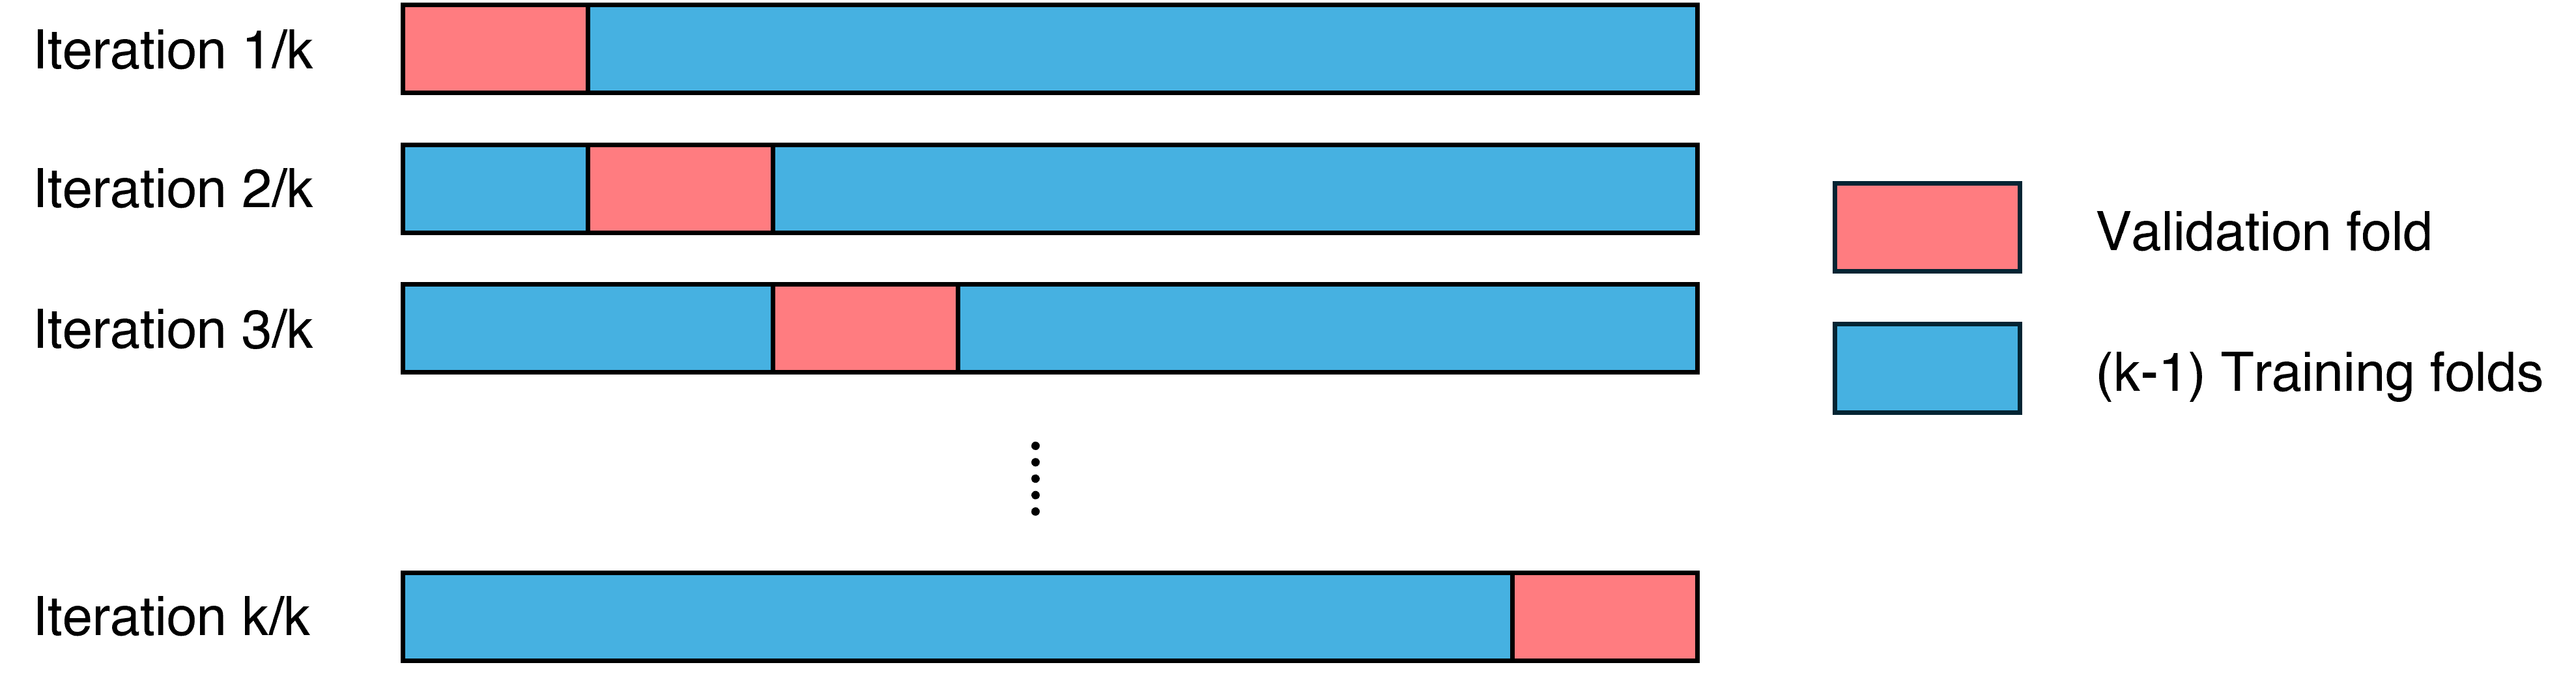
\includegraphics[width=10cm]{images/Theory-DL/crossval.png}
  \caption{Schematic Representation of LOOCV - Here, the training and validation datasets are taken together and split into k folds. The model is trained k times and in each iteration, exactly one fold is subsequently chosen as the validation fold (depicted in red) while the remaining (k-1) folds (depicted in blue) are combined to become the training dataset.}
  \label{fig:crossval}
\end{figure}
\subsection{Optimization} 
Optimization involves adjusting the parameters of the neural network, such as weights and biases, to minimize a predefined objective function, typically referred to as the loss function. The optimization process iteratively updates the parameters based on the gradients of the loss function with respect to the network's parameters, aiming to converge to a set of optimal parameters that yield the best performance on the given task. Some important aspects of the optimization process are discussed in the following subsections. 
\subsubsection{Loss function}
The loss function quantifies the difference between the model's predictions and the actual target values. It represents the measure of how well the model is performing on the training data. Common loss functions include mean squared error (MSE) for regression tasks and categorical cross-entropy for classification tasks. The loss function $\mathcal{L}(\theta)$ is defined as: 
\begin{equation}
    \mathcal{L}(\theta)=\frac{1}{N} \sum_{i=1}^N L\left(y_i, \hat{y}_i ; \theta\right)
    \end{equation}
Here, $\theta$ represents the parameters of the neural network being optimized, such as weights and biases, $y_i$ is the ground truth and $\hat{y}_i $ is the model prediction. The loss function $\mathcal{L}(\theta)$ depends on these parameters, and it is computed as the average of the individual loss $L\left(y_i, \hat{y}_i ; \theta\right)$ over all the training examples, of size $N$.
\subsubsection{Backpropagation}
Backpropagation is a fundamental algorithm used to compute the gradients of the loss function with respect to the parameters (weights and biases) of the neural network. It involves propagating the error backward from the output layer to the input layer, updating the parameters along the way to minimize the loss. The gradients are computed using the chain rule of calculus, enabling efficient optimization of the network's parameters. Mathematically, the gradients $\nabla_\theta \mathcal{L}(\theta)$ of the loss function are computed as,
\begin{equation}
    \nabla_\theta \mathcal{L}(\theta)=\frac{1}{N} \sum_{i=1}^N \nabla_\theta L\left(y_i, \hat{y}_i ; \theta\right)
    \end{equation}
\subsubsection{Learning rate}
The learning rate is a hyperparameter that controls the size of the parameter updates, that is, the step-size in the direction of the gradients computed by backpropagation. A higher learning rate may lead to faster convergence but risks overshooting the optimal solution, while a lower learning rate may result in slower convergence but more stable training. The parameter update rule with learning rate $\eta$ is given by:
\begin{equation}
    \theta_{t+1}=\theta_t-\eta \nabla_\theta \mathcal{L}(\theta)
    \end{equation}
Here, $\theta_{t+1}$ and $\theta_t$ represent the parameters at time step $t$ and $t+1$ respectively. Learning rate decay is often used to gradually reduce the learning rate during training with the help of learning rate schedulers such as,
\begin{itemize}
\item \textbf{Step decay} reduces the learning rate by a factor (typically constant) after a fixed number of epochs or iterations.
\item \textbf{Exponential decay} reduces the learning rate exponentially over time.
\end{itemize}
% \begin{figure}[ht]
%   \centering
%   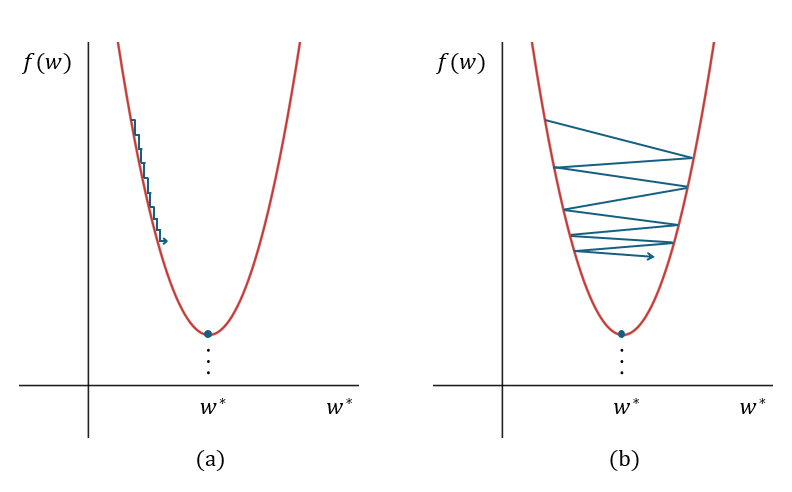
\includegraphics[width=10cm]{images/Theory-DL/LR.png}
%   \caption{Effect of Learning Rates}
%   \label{fig:LR}
%   \end{figure}
\subsubsection{Optimizer} 
The optimizer is responsible for updating the parameters of the neural network based on the gradients computed during backpropagation. It determines the direction and magnitude of parameter updates to minimize the loss function efficiently. Popular optimizers include \gls{SGD} \cite{sgd}, \gls{Adam} \cite{adam}, \gls{RMSProp} \cite{rmsprop}, and \gls{AdaGrad} \cite{adagrad}. We use the Adam optimizer in the training and testing phases of our work. \\
 \textbf{Adam (Adaptive Moment Estimation)} is an algorithm for stochastic optimization that combines the ideas of SGD with momentum and RMSProp. It maintains exponentially decaying moving averages of past gradients and past squared gradients for each parameter. These moving averages serve as estimates of the first moment (the mean) and the second moment (the uncentered variance) of the gradients, respectively. Adam also incorporates bias correction terms to compensate for the initial bias towards zero at the beginning of training. The parameter update rules at time step $t$ are given by,
 \begin{enumerate}
  \item Compute the gradient of the loss function with respect to the parameters, \(\theta_t\).
  \item Update biased first moment estimate: \(m_t = \beta_1 m_{t-1} + (1 - \beta_1)\theta_t\).
  \item Update biased second raw moment estimate: \(v_t = \beta_2 v_{t-1} + (1 - \beta_2)\theta_t^2\).
  \item Compute bias-corrected first moment estimate: \(\hat{m}_t = \frac{m_t}{(1 - \beta_1^t)}\).
  \item Compute bias-corrected second moment estimate: \(\hat{v}_t = \frac{v_t}{(1 - \beta_2^t)}\).
  \item Update the parameters: \(\theta_{t+1} = \theta_t - \eta \cdot \frac{\hat{m}_t}{(\sqrt{\hat{v}_t} + \epsilon)}\).
\end{enumerate}
Here, \(m_t\) and \(v_t\) are estimates of the first moment (the mean) and the second moment (the uncentered mean and variance) of the gradients, respectively. \(\beta_1\) and \(\beta_2\) are exponential decay rates for these moment estimates, typically close to 1. $\hat{m}_t$ and $\hat{v}_t$ refer to the bias-corrected estimates of the first and second moments (uncentered variance) of the gradients, and $\epsilon$ is a small constant to prevent division by zero.
\section{Model evaluation metrics}
Model evaluation metrics are essential for assessing the performance of deep learning models. The loss function serves as a crucial metric for evaluating model performance, in addition to optimizing model parameters during training. In regression tasks, where the goal is to predict continuous values, common loss functions include the following:
\begin{itemize}
\item \textbf{\gls{MAE}:} MAE measures the average absolute difference between the predicted values and the actual values:\[ \text{MAE} = \frac{1}{N} \sum_{i=1}^{N} |y_i - \hat{y}_i| \] Here, $y_i$ are the ground truth values, $\hat{y}_i$ are the predicted values, and $n$ is the number of samples. MAE is robust to outliers and does not penalize large errors heavily.
% \textbf{Mean Relative Error (MRE)}
\item \textbf{\gls{MSE}:} MSE measures the average squared difference between the predicted values and the actual values:\[ \text{MSE} = \frac{1}{N} \sum_{i=1}^{N} (y_i - \hat{y}_i)^2 \] MSE penalizes larger errors more heavily than MAE since errors are squared. This makes it more sensitive to outliers. 
\item \textbf{\gls{RMSE}:} RMSE is the square root of the average squared difference between the predicted values and the actual values: \[ \text{RMSE} = \sqrt{\frac{1}{N} \sum_{i=1}^{N} (y_i - \hat{y}_i)^2} \]RMSE is sensitive to outliers, similar to MSE, but is more interpretable as it is in the same units as the target variable.
\end{itemize}
\section{Convolutional Neural Networks (CNNs)} \label{cnnse}
\gls{CNN}s \cite{lecun1998} are specialized neural networks designed to process grid-like data, such as images. They utilize convolutional layers and pooling operators to learn spatial hierarchies of features from input data, making them highly effective for tasks like image classification, object detection, and image segmentation.
\begin{figure}[ht]
    \centering
    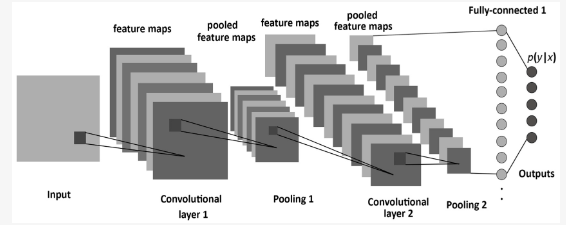
\includegraphics[width=10cm]{images/Theory-DL/CNN.png}
    \caption{Diagram illustrating the typical structure of a CNN consisting of convolutional, pooling, and fully connected layers. Image taken from \cite{cnnimage}.}
    \label{fig:CNN}
  \end{figure}
\subsection{Convolutional layer}
The convolutional layer in a CNN consists of a set of learnable filters (kernels) that slide over the input data, performing element-wise multiplication and summing to produce feature maps. The convolution operation preserves the spatial relationship between pixels and learns local patterns like edges, textures, and shapes. Figure \ref{fig:Conv1} shows the working of a convolution kernel. 
\begin{figure}[ht]
    \centeringflo
    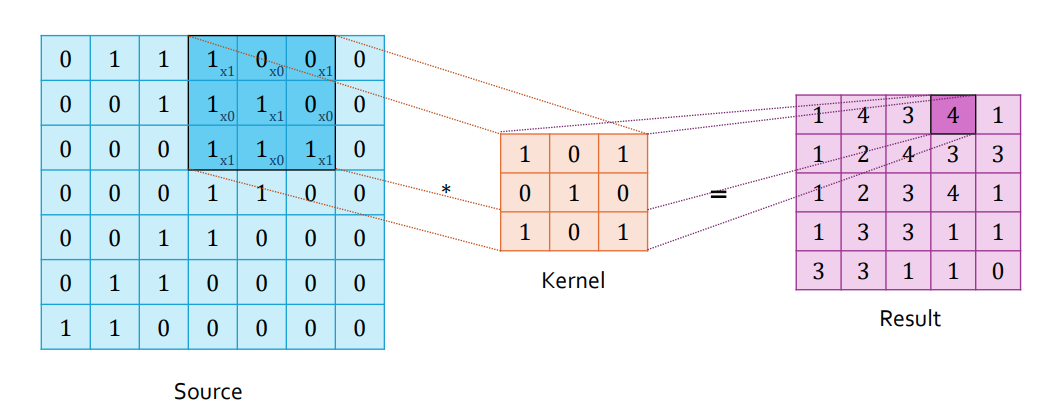
\includegraphics[width=14cm]{images/Theory-DL/Conv1.png}
    \caption{Detailed view of a convolutional layer's operation in a CNN, depicting the convolution process over an input matrix with a specified kernel to produce feature maps.}
    \label{fig:Conv1}
  \end{figure}
\subsection{Pooling and unpooling} Pooling and unpooling operators perform effective downsampling and upsampling operations respectively, enabling hierarchical feature extraction while preserving spatial information. Pooling is a down-sampling operation commonly used in CNNs to reduce the spatial dimensions of feature maps. Max pooling and average pooling are popular pooling techniques that select the maximum or average value within each pooling region, respectively. These operations are depicted in Figure \ref{fig:Pool}. Conversely, unpooling layers, often used in upsampling, aim to reconstruct the original input resolution from the lower-dimensional representations generated by pooling. These layers typically store the indices of the maximum values during pooling and use them for upsampling. Nearest neighbor interpolation is a simpler upsampling method where each pixel in the input is replicated multiple times to form the output as can be seen in Figure \ref{fig:Unpool2}.
\begin{figure}[ht]
    \centering
    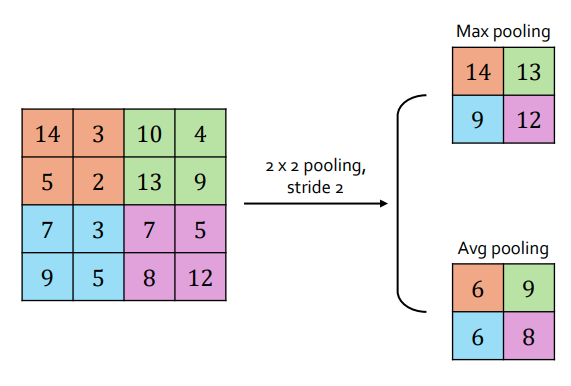
\includegraphics[width=8cm]{images/Theory-DL/Pool.png}
    \caption{Visualization of pooling operations for downsampling spatial dimensions in CNNs, with examples of (a) max pooling, and (b) average pooling.}
    \label{fig:Pool}
\end{figure}
\begin{figure}[ht]
        \centering
        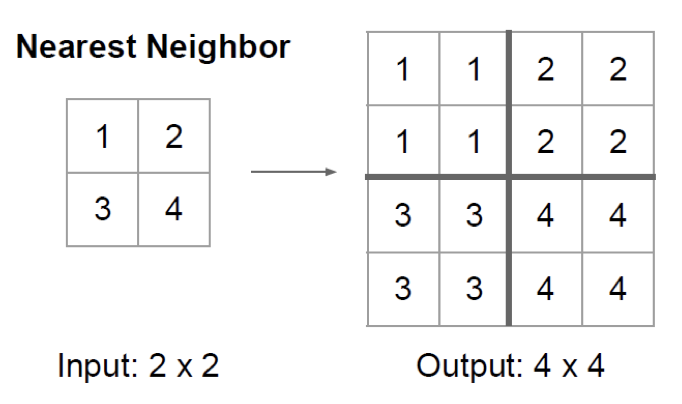
\includegraphics[width=8cm]{images/Theory-DL/NNUnpool.png}
        \caption{Illustration of the unpooling process of nearest neighbor interpolation, used for upsampling in CNNs.}
        \label{fig:Unpool2}
    \end{figure}
\subsection{The U-Net architecture}
U-Net \cite{unet} is a CNN consisting of a U-shaped network structure with a contracting path (encoder) followed by an expanding path (decoder), which enables precise segmentation of structures in medical images, such as cells, organs, or tumors. Some important components of the U-Net architecture are discussed below. 
\begin{figure}[ht]
    \centering
    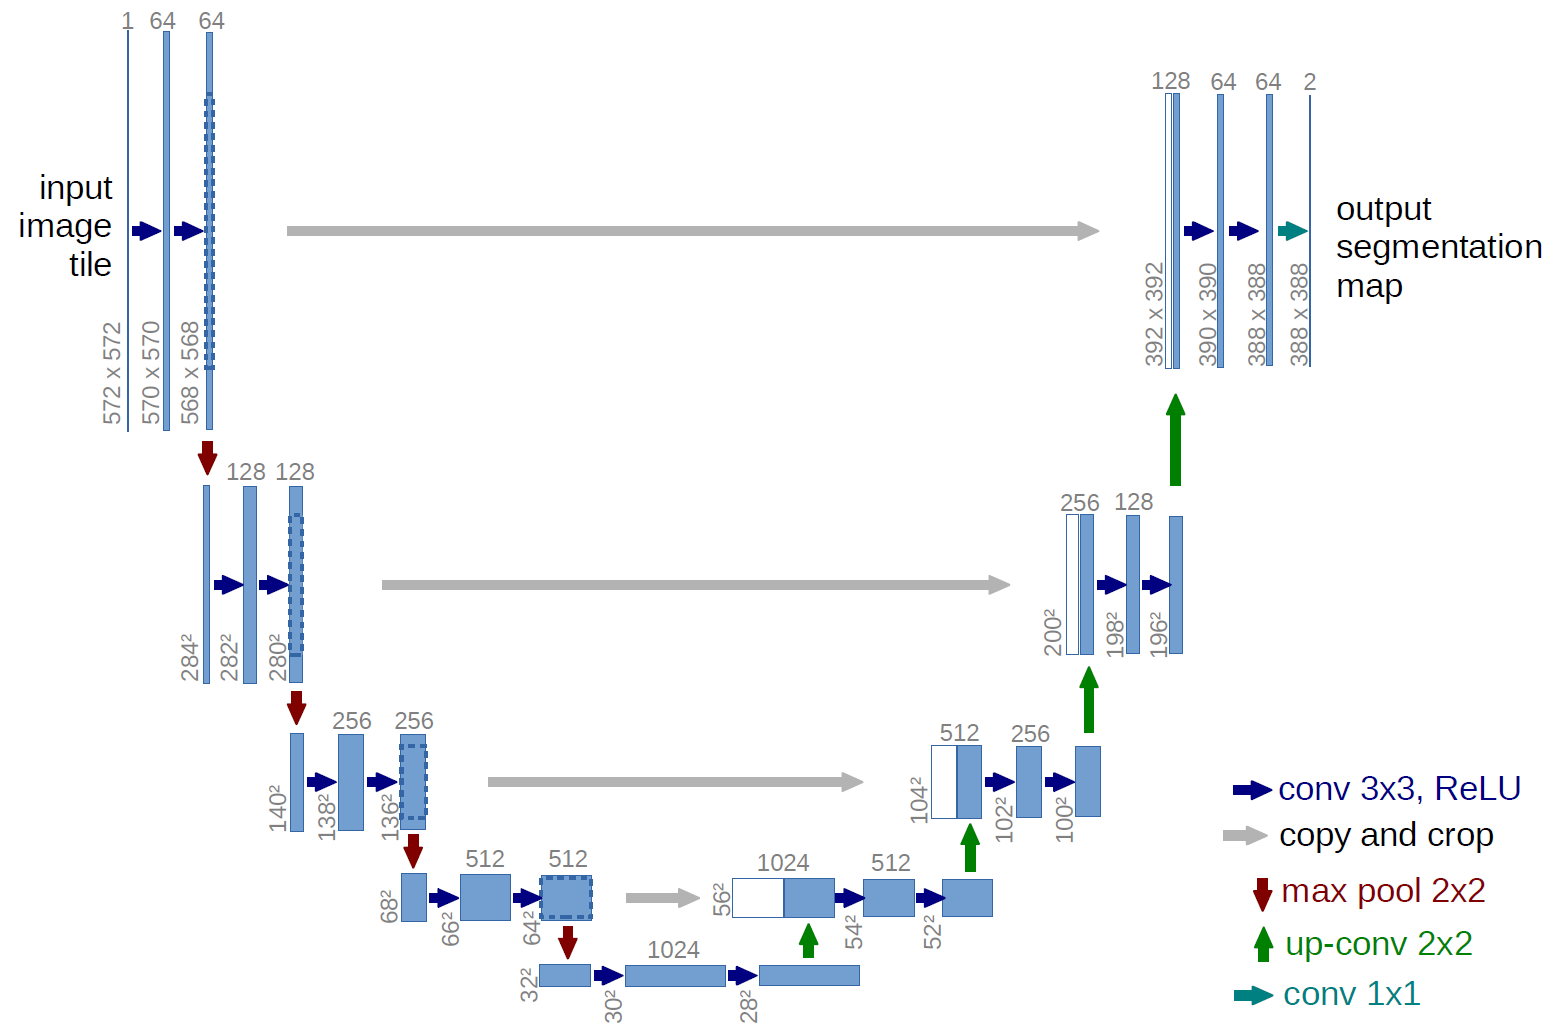
\includegraphics[width=12cm]{images/Theory-DL/UNet.png}
    \caption{Structure of the U-Net architecture demonstrating its U-shaped design with contracting and expanding paths. Image taken from \cite{unet}.}
    \label{fig:UNet}
\end{figure}
\begin{enumerate}
  \item The \textbf{encoder} comprises a series of down-convolutional and max pooling layers that gradually reduce the spatial dimensions of the input image while increasing the number of feature channels. This path extracts high-level features from the input image while preserving spatial context.
  \item The \textbf{decoder} consists of up-convolutional (transposed convolution) and concatenation layers that gradually increase the spatial dimensions of the feature maps while reducing the number of feature channels. This path generates segmentation masks by upsampling the low-resolution feature maps obtained from the encoder and combining them with high-resolution feature maps using skip connections.
  \item \textbf{Skip connections} or residual connections \cite{he2016deep}, are direct connections between layers at the same hierarchical level in the network. In the U-Net architecture, skip connections connect the encoder to the corresponding layers in the decoder. This enables the network to retain fine-grained spatial information from the encoder while recovering spatial details lost during downsampling. By directly linking the encoder and decoder layers, skip connections facilitate the flow of information across different scales, improving the model's ability to capture both local and global context.
\end{enumerate}
\begin{figure}[ht]
    \centering
    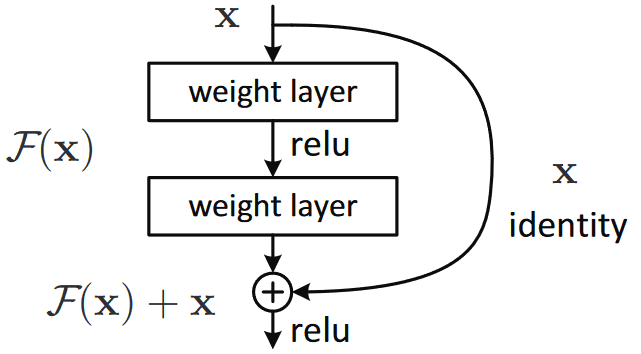
\includegraphics[width=6cm]{images/Theory-DL/Skip.png}
    \caption{Diagram demonstrating the concept of skip connections within neural network architectures. Skip connections bypass one or more layers by directly feeding the output from an earlier layer to a later layer.} 
    \label{fig:Skip}
\end{figure}
A notable observation pertinent to our current endeavor is the striking resemblance between the U-Net architecture and the V-cycle multi-grid method, as noted by He and Xu \cite{HeXu2019}. Both employ a hierarchical structure wherein information is exchanged across varying resolutions.
\section{Graph Neural Networks (GNNs)} \label{gnnse}
A major limitation of CNNs is their inability to directly operate on irregular data formats, such as social networks, recommender systems, molecular structures, or citation networks. In 2017, Kipf and Welling \cite{kipf} introduced the Graph Convolutional Network (GCN), a foundational architecture that laid the groundwork for modern GNNs. Since then, numerous advancements and variants of GNNs have been proposed. In contrast to CNNs which are well-suited for grid-like structured data such as images, GNNs are tailored for data represented as graphs, which are characterized by non-Euclidean and irregular structures, where entities (nodes) and their relationships (edges) vary in connectivity and structure. \gls{GNN}s excel in processing unstructured data by leveraging the inherent graph structure by dynamically aggregating information from neighboring nodes based on their connectivity. \\
Graphs are set up using nodes, edges, adjacency matrices, node attributes, and edge attributes. 
\begin{enumerate}
  \item \textbf{Nodes (\(V\))}: Nodes represent entities in a graph, such as users in a social network, atoms in a molecule, or words in a document. Formally, a graph can be denoted as \( G = (V, E) \), where \( V \) is the set of nodes.
  \item \textbf{Edges (\(E\))}: Edges define relationships or connections between nodes in a graph. Each edge \( e_{ij} \) connects node \( v_i \) to node \( v_j \), where \( v_i, v_j \in V \). The edge set \( E \) can be represented as a collection of tuples \( (v_i, v_j) \) indicating the connections between nodes.
  \item \textbf{Adjacency matrix (\(A\))}: An adjacency matrix is a binary $n \times n$ matrix representing the connections between nodes in a graph. For an undirected graph, \( A_{ij} \) is 1 if there exists an edge between nodes \( v_i \) and \( v_j \), and 0 otherwise. For directed graphs, the adjacency matrix may be asymmetric to represent the directionality of edges. The adjacency matrix \( A \) of a graph \( G = (V, E) \) can be defined as,
  \[
  A_{ij} = \begin{cases} 1 & \text{if } (v_i, v_j) \in E \\ 0 & \text{otherwise} \end{cases}
  \]
  \item \textbf{Node attributes and feature matrix(\(X\))}: Node attributes or features represent information associated with each node in the graph. These features can encode characteristics such as velocity, pressure, and temperature as node embeddings. The node feature matrix $X$ for a graph with \( N \) nodes and \( D \) features is a $N \times D$ matrix where each row corresponds to a node and each column represents a feature dimension, given by,
\begin{equation*}
  X = \begin{bmatrix} x_1^T \\ x_2^T \\ \vdots \\ x_N^T \end{bmatrix} \quad \text{ where,} \quad x_i = \begin{bmatrix} x_{i1} \\ x_{i2} \\ \vdots \\ x_{iD} \end{bmatrix}
\end{equation*}
where \( x_i \) represents the feature vector associated with node \(v_i \).
  \item \textbf{Edge weights or attributes (\(W\))}: Edge weights quantify the strength or intensity of relationships between nodes connected by edges. These weights can represent similarity measures, distances, or any other relevant information associated with edge connections. Similar to node weights, edge weights can be learned or predefined. 
\end{enumerate}  
\begin{figure}[ht]
  \centering
  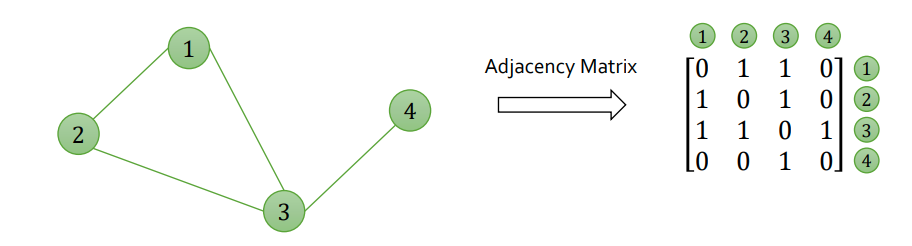
\includegraphics[width=12cm]{images/Theory-DL/AdjMat.png}
  \caption{Demonstration of an adjacency matrix representing graph connectivity and the binary representation of node relationships in graph-structured data.}
  \label{fig:AdjMat}
\end{figure}
GNNs leverage these components to perform message passing and aggregation operations across the graph structure, which are discussed below. \\
\subsection{Graph convolutions}
Graph convolutions update the feature representations of nodes in a graph by aggregating information from their neighboring nodes. There are two ways to perform graph convolution operations. In spectral convolution, graph signals are transformed into the spectral domain using techniques like graph Fourier transforms. Spatial convolution directly operates on the graph's topology and neighborhood structure, aggregating information from neighboring nodes without explicitly transforming the graph. \gls{GCN}, \gls{GAT}, and GraphSAGE are some common classes of GNNs that utilize spatial convolutions. In this work, we only deal with spatial convolutions and refer to them as graph convolutions henceforth. The main steps involved in graph convolutions are as follows:
\begin{enumerate}
    \item \textbf{Message passing}: Nodes exchange messages with their neighbors, aggregating information from neighboring nodes. The message passed from node $v_j$ to node $v_i$ can be represented as:
        \[ m_{ij} = \frac{1}{c_{ij}} W h_j \]
        where $m_{ij}$ is the message from node $j$ to node $i$, $W$ is the learnable weight matrix, and $c_{ij}$ is a normalization factor.
    
    \item \textbf{Aggregation}:Nodes aggregate the messages received from their neighbors to update their own feature representations. The aggregated message $a_i$ for node $i$ can be computed as the sum or average of the incoming messages.
        \[ a_i = \sum_{j \in \mathcal{N}(i)} m_{ij} \]
    where $\mathcal{N}(i)$ denotes the set of neighboring nodes of $v_i$.
    \item \textbf{Update}: Nodes update their feature representations using the aggregated messages and their own features. The updated feature representation $h_i^{(l+1)}$ for node $i$ at layer $l+1$ can be computed as:
        \[ h_i^{(l+1)} = \sigma(a_i) \]
\end{enumerate}
These steps are performed iteratively across multiple layers of the GNN. At each layer, nodes update their feature representations based on the aggregated messages. The iterative propagation of messages allows nodes to incorporate information from distant parts of the graph and refine their representations over multiple layers. \\
Graph convolution operators typically exhibit local connectivity, where each node's representation is updated based on the information from its neighboring nodes.
This local connectivity property allows the model to capture localized patterns and dependencies within the graph structure. Weight sharing is a key aspect of graph convolutions, where the same set of learnable parameters (weights) is shared across different nodes in the graph. This allows for parameter efficiency and enables the model to generalize well to unseen nodes and graphs. 
% \subsection{Message passing}
% Message passing is a fundamental operation in GNNs where nodes exchange information with their neighbors in the graph. This mechanism enables nodes to aggregate and propagate information across the graph, allowing them to update their representations based on the local neighborhood structure. 
%%% \textbf{Message Computation:} Each node aggregates information from its neighboring nodes to compute a message. This aggregation process involves applying a function to combine features of neighboring nodes.\\
%%% \textbf{Message Aggregation:} After computing messages, each node aggregates the received messages to update its own representation. This aggregation operation typically involves summing or averaging the incoming messages. \\
% The message passing process can be represented as follows:
% \[
% m_{v \rightarrow u}^{(l)} = M^{(l)}(h_v^{(l)}, h_u^{(l-1)}, e_{vu})
% \]
% where,
% \begin{itemize}
%     \item $m_{v \rightarrow u}^{(l)}$ represents the message sent from node $v$ to node $u$ at layer $l$,
%     \item $M^{(l)}$ is a message function applied to the features of nodes $v$ and $u$ and the corresponding edge $e_{vu}$,
%     \item $h_v^{(l)}$ and $h_u^{(l-1)}$ are the feature vectors of nodes $v$ and $u$ at layers $l$ and $l-1$, respectively.
% \end{itemize}
% After computing messages, the aggregated message for node $u$ is obtained by combining messages from all neighboring nodes:
% \[
% m_u^{(l)} = \sum_{v \in \mathcal{N}(u)} m_{v \rightarrow u}^{(l)}
% \]
% where $\mathcal{N}(u)$ denotes the set of neighboring nodes of $u$.

\subsection{Graph pooling}
Graph pooling aggregates node representations across the entire graph to compute global graph-level features and create a coarser graph representation. It reduces the size of the graph representation while preserving important structural and relational information. By selecting representative nodes or aggregating node features, graph pooling enables GNNs to focus on relevant information while reducing computational complexity. Graph pooling also facilitates hierarchical feature learning by allowing GNNs to operate at multiple levels of granularity, enabling the model to capture both local and global patterns in the graph. The different types of graph pooling are:
\begin{enumerate}
\item \textbf{Top-k pooling} selects the top k nodes based on criteria such as node importance or feature values, and aggregates their information to create a coarser graph representation. This method retains the most informative nodes while reducing the size of the graph, making it suitable for tasks requiring node selection or summarization.
\item \textbf{Max pooling} selects the node with the maximum feature value from each neighborhood and aggregates their information to create a coarser representation of the graph. It emphasizes the most salient nodes in each neighborhood, capturing important features while reducing redundancy.
\item \textbf{Self-attention graph pooling} leverages attention mechanisms to dynamically weight the contributions of neighboring nodes based on their importance and similarity. It allows nodes to attend to relevant information in their neighborhoods, facilitating adaptive aggregation and effective summarization of the graph. This method is useful for capturing long-range dependencies and global patterns in the graph.
\end{enumerate}
% Graph pooling aggregates node features to produce a compact representation of the entire graph, which can be fed into subsequent layers or used for downstream tasks. \\
Graph unpooling is a complementary operation to graph pooling, aimed at upsampling or reconstructing the original graph representation after downsampling. While graph pooling creates a coarser representation, graph unpooling aims to recover the finer details and restore the original graph structure. Some common types of graph unpooling include,
\begin{enumerate}
\item \textbf{Max unpooling} is an unpooling strategy used in conjunction with max pooling. During max pooling, the locations of the maximum activations are stored. In max unpooling, these locations serve as masks to place the pooled values back into their original positions in the unpooled feature map.
\item \textbf{Nearest neighbor interpolation} aims to recover the original graph topology by identifying the nearest neighbors of pooled nodes in the coarse representation and reinstating unpooled nodes based on their proximity. It reconstructs edges between unpooled nodes and their nearest neighbors, restoring connectivity and preserving local structure.
%  Nearest neighbor unpooling is effective in capturing local relationships and structural patterns in the graph.
\end{enumerate}
% \subsection{Message Passing}
% \subsection{Graph Convolutions}
% \subsection{Graph Pooling and Unpooling}
\subsection{Hierarchical multi-resolution approach} 
\label{SO}
Multi-resolution approaches in the context of GNNs involve operating on graphs at multiple levels of granularity, similar to the multigrid method in numerical analysis. 
% In extending the multi-grid concept to the GNNs, a different approach is necessary compared to Convolutional Neural Networks (CNNs). 
Unlike CNNs, where downsampling operators automatically coarsen the mesh, in GNNs, we create a hierarchy of meshes with increasing complexity over the domain of interest. Hence, traditional pooling operators may not be suitable for GNNs, as they focus on selecting nodes to construct a coarse graph, which is unnecessary for mesh data. Instead, we can easily define operators that transform features from one mesh to the next, by generating a set of meshes with varying coarseness.\\
Creating a mesh hierarchy of different levels of coarseness can be performed by well-established techniques in numerical analysis. One commonly used algorithm for mesh construction is Delaunay triangulation, which maximizes the minimum angle of all triangles to avoid sliver triangles. This algorithm gradually inserts new nodes into the triangulation and connects them with their neighbors under specific rules. Incremental decimation is another mesh coarsening method that aims to reduce the number of points while preserving specific properties of the original mesh. It iteratively removes one vertex or edge with minimal changes until certain criteria are met. These techniques offer flexibility in creating mesh hierarchies, making them suitable for GNNs applied to mesh data.\\
\subsubsection{Sampling operator}
We introduce a sampling operator for converting data between two meshes, denoted as $M_1$ and $M_2$, inspired by the k-nearest interpolation proposed in PointNet++ \cite{pnpp}. Let \(z\) be a node from \(M_1\), and assume its \(k\) nearest neighbors on \(M_2\) are denoted as \(x_1, \ldots, x_k\). For a node feature \(f\), the interpolated feature \(f(z)\) is defined based on the features of \(x_i\) as,
\begin{equation}
  \mathbf{f}(\mathbf{z})=\frac{\sum_{i=1}^k w\left(x_i\right) \mathbf{f}\left(x_i\right)}{\sum_{i=1}^k w\left(x_i\right)} \text {, where } w\left(x_i\right)=\frac{1}{\left\|z-x_i\right\|_2}
  \end{equation}
With these operators, both upsampling and downsampling operators can be defined straightforwardly for developing multi-resolution architectures for mesh-based problems.

%% ---------------------------------------------------------------------------
%%
%% Methodology
%%
%% ---------------------------------------------------------------------------
\part[Methodology]{Methodology and Implementation}
\label{part:Method}
\chapter{Implementation, results and discussion}
\label{chap:Method}
This chapter begins with the detailed exploration of the processes and methodologies employed to implement GNNs for the predictive analysis of nozzle flows. In the subsequent section, we introduce the Graph U-Net architecture, outline its implementation settings, present the results obtained and corroborate them with the simulation outcomes. This discussion sets the stage for the development of three modified surrogate models with the aim of enhancing model performance, detailed in Section \ref{proparch}. Through quantitative analysis and performance evaluation, we identify the successes and challenges encountered in modeling nozzle flow dynamics with GNNs. Thus, this chapter demonstrates the practical implementation of the proposed methodologies and performs a critical examination of the results and the efficacy of these models.
\section{Data pre-processing} \label{prep}
In this section, we describe the process for dataset preparation, how the data from CFD simulations are extracted and converted into graph-structured formats that facilitate efficient GNN training. It includes dataset generation from nozzle flow simulations at varied conditions, transformation of unstructured mesh data into a graph format for GNN compatibility, and the specification of GNN inputs and outputs. 
\subsection{Dataset generation}
Nozzle simulations are carried out for 120 cases, each with a different set of Inlet 1 and Inlet 2 velocities. The velocity ratio between the two velocities lies in the range of [1,10]. Velocity ratio in our case refers to the ratio of higher velocity to that of lower velocity.
%  such that the velocity ratios between the inlets range from 1 to 9.  (Velocity ratio in our case refers to the ratio of higher velocity to that of lower velocity) 
% The simulation results, i.e; the steady-state fields are logged after 1000 and 30000 time-steps. The \gls{CFD} results at 1000 time-steps are still developing and are unstable whereas those at 30000 steps are observed to be stable solutions. Hence, the simulation results after 30000 steps are taken as the ground truth values or target data, while the input to the surrogate model are the results after 1000 steps. The input and target datasets are then transformed into graph data, normalized, and passed to the network. 
Simulation data are obtained at two intervals: after 1000 and 30000 iterations or steps. The results at 1000 iterations, which are still developing and unstable, serve as inputs to the surrogate model. Whereas, the results at 30000 iterations, which represent stable solutions, are considered the ground truth or target data for model training. These results are then transformed into graph data, which encapsulate spatial relationships and properties of flow fields. The GNN architecture is designed to learn these features and predict the stable, steady-state fields from the early, unstable simulation results.
\subsection{Transformation of mesh data to graph data}
Conventional RANS solvers require substantial distances from domain boundaries to mitigate adverse effects on solutions around the region of interest. However, this is not required for the deep learning task. Hence, we narrow our attention to a small region just enclosing the nozzle as seen in Figure \ref{clipmesh}. We clip the CFD mesh appropriately and resample the velocity and pressure fields to this mesh with reduced spatial extent. We define the cell-centers on the clipped mesh and assign them as the nodes of the graph. Two adjacent cells $i$ and $j$ (cells that share an edge) in this resulting unstructured mesh are represented as nodes $v_i$ and $v_j$ on the graph and are connected by an edge $e_{ij}$. The graph connectivity is then given by the edge index data structure which comprises two lists - one stores the source node indices and the other has the destination node indices. CFD solvers typically assign pressure, velocity and other fields to each cell of the mesh, whereas graphs require node features, i.e; fields defined on each node. Therefore, the cell data (fields) are converted to point data at the cell centers making it suitable for graph representation. The simulation data is then saved in a \verb|hdf5| format. This is then directly used to read pressure, velocity and co-ordinate information at cell centers. 
% $u_{x}$, $u_{y}$, $p$, $c_x$, $c_y$, and $\gamma_{\operatorname{tag}}$. 
The edge index data required for the GNN is generated by computing adjacent cells and storing their indices in a \gls{COO} format. 
\begin{figure}[ht]
    \centering
    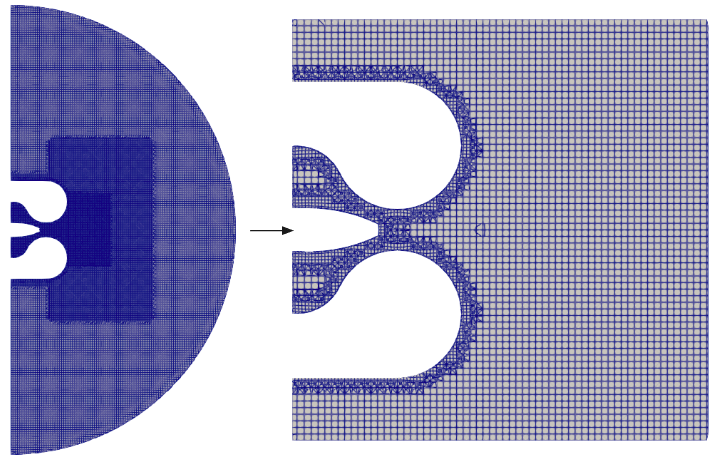
\includegraphics[width=11cm]{images/Methodology/Clipped.png}
    \caption{Depiction of the area of focus - the original CFD mesh (left) is clipped and transformed into the region of interest (right)}
    \label{clipmesh}
\end{figure}
\begin{figure}[ht]
    \centering
    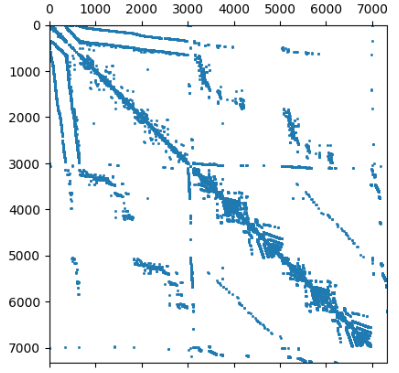
\includegraphics[width=6cm]{images/Methodology/AdjMatrix.png}
    \caption{Visualization of the adjacency matrix representing the graph connectivity of the clipped, unstructured mesh with 7329 nodes.}
    \label{adjmat}
\end{figure}
\subsection{Model inputs and outputs}
After data pre-processing, the simulation mesh is considered as a bidirectional graph $\mathbf{G} = (\mathbf{V}, \mathbf{E})$ where the set of $N$ nodes denoted as $\mathbf{V}$ are linked by the set of edges $\mathbf{E}$ of the graph. To construct a graph, we need,
\begin{itemize}
\item A feature description, consolidated into an $N \times D$ feature matrix $X$, where $D$ denotes the number of input features.
\item The graph connectivity or relationships within nodes is represented in matrix form as an adjacency matrix, $A$ or as an edge set $E$ of the shape $2 \times P$, where $P$ is the number of pairs of connected nodes in $E$.
\end{itemize}
Let each node have $F_X$ features, and $F_Y$ predictions. The GNN maps the set of node features and edge index matrices to predictions as, 
\begin{equation}
    \mathrm{GNN}: \mathbb{R}^{{N} \times F_{\mathrm{X}}}, \mathbb{W}^{2 \times P} \rightarrow \mathbb{R}^{{N} \times F_{\mathrm{Y}}}
    \end{equation}
We then get a graph-level output $Z$ of the shape ${N} \times F_{\mathrm{Y}}$. \\
The node feature vector $\mathbf{x}_i$ and prediction vector $\mathbf{y}_i$ of interest at each node $v_i$ is given as,
\begin{equation}
    \begin{aligned}
    & \mathbf{x}_i=\left[u_{x, i}, u_{y, i},c_{x, i}, c_{y, i}, \gamma_{\operatorname{tag}, i}\right] \\
    & \mathbf{y}_i=\left[u_{x, i}, u_{y, i}, p_i\right]
    \end{aligned}
\end{equation}
where $u_{x, i}$ and $u_{y, i}$ are the node velocities in X and Y directions, $c_{x, i}$ and $c_{y, i}$ are the spatial co-ordinates of the nodes and $p_i$ is the node pressure. $\gamma_{\operatorname{tag}, i}$ is the node tag that defines which cell the node belongs to: inlet, walls or internal mesh. To summarize, our model has 5 input channels (representing node features) and 3 output channels (denoting node predictions). In addition to these channels, the GNN model also requires an edge index matrix to internally compute the adjacency matrix for the graph. 
\subsection{Data normalization}
Data normalization is performed on both input channels (node features) and output channels (target vectors), carried out in three steps outlined below.
\begin{enumerate}
\item Following common practice, we normalize all the fields of interest with respect to the magnitude of free-stream or reference velocity $u_0$ to make them dimensionless. 
\begin{equation}
    \Tilde{u}=u /\left\|u_0\right\|, \quad \Tilde{p}=p /\left\|u_0\right\|^2
\end{equation}
The latter plays a crucial role as it eliminates the quadratic scaling effect present in the pressure values of the target data, effectively flattening the solution space, thereby simplifying the task for the neural network in subsequent stages.
\item Next, we subtract the mean pressure from the dimensionless pressure values. 
\begin{equation}
\hat{p} = \Tilde{p} - p_{mean} , \quad \text{where} \quad p_{mean} = \sum_i p_i / n
\end{equation}
$n$ is the number of training samples and $p_i$ denotes individual pressure values. Without this step, the pressure targets depict an ill-posed learning objective since the random pressure offsets in the solutions lack correlation with the inputs.
\item As a final step, every channel undergoes normalization to the range of [-1, 1] or [0,1]. This standardization aims to mitigate errors stemming from finite numerical precision during the training period. We opt for the maximum absolute value of each quantity across the entire training dataset to normalize the data. 
\end{enumerate}
After performing normalization, we shuffle the entire dataset split it into 3 parts and distributed as training data, validation data and test data in the ratio of 80:10:10. 
\section{Graph U-Net}
Here, we introduce the Graph U-Net architecture, a foundational framework for the surrogate models used in this work. We analyze the benefits and shortcomings of this model as well as explain the motivation behind developing a modified GNN.
% Some important aspects of graph convolutions are detailed below. 
% \begin{enumerate}
% \item \textbf{Aggregation of neighbor information:} Each node aggregates the features of its neighbors, weighted by the parameters learned in the weight matrix $W^{(l)}$. This process enables nodes to incorporate information from their local neighborhoods, capturing relational dependencies and structural patterns in the graph. 

% % The normalization factor $c_{ij}$ ensures that the aggregated features are appropriately scaled based on the connectivity of nodes.
% \item \textbf{Weight sharing:}
% The weight matrix $W^{(l)}$ is shared across all nodes, allowing the model to capture common patterns and relationships present in the graph. By sharing parameters, GCNs can effectively learn representations from limited labeled data, facilitating transfer learning and adaptation to new graphs or domains.
% \item \textbf{Hierarchical feature learning:}
% GCNConv layer enables hierarchical feature learning by iteratively aggregating information from neighboring nodes. As information propagates through multiple layers, nodes can capture increasingly abstract and high-level features of the graph. 
% \end{enumerate}
\subsection{Architecture}
The downsampling operation is carried out using the top-k pooling strategy, which retains the most important nodes in the graph while discarding less relevant nodes based on a specified criterion. GCNConv layers are used as the convolutional layers in Graph U-Nets. Here, unpooling is not a distinct operation like in traditional U-Nets. Instead, skip connections are used to implicitly perform unpooling. During decoding, downsampled features from the encoder are combined with zeros or empty features in the decoder using skip connections. This integration effectively restores spatial details and contextual information from the original input graph, ensuring that important features are retained and allowing for the recovery of detailed graph structures. Therefore, unpooling in Graph U-Net is seamlessly integrated into the skip connection mechanism, facilitating the reconstruction of the original graph resolution during decoding. Figure \ref{fig:GraphUnet} presents a schematic overview of the Graph U-Net architecture. 
\begin{figure}[ht]
    \centering
    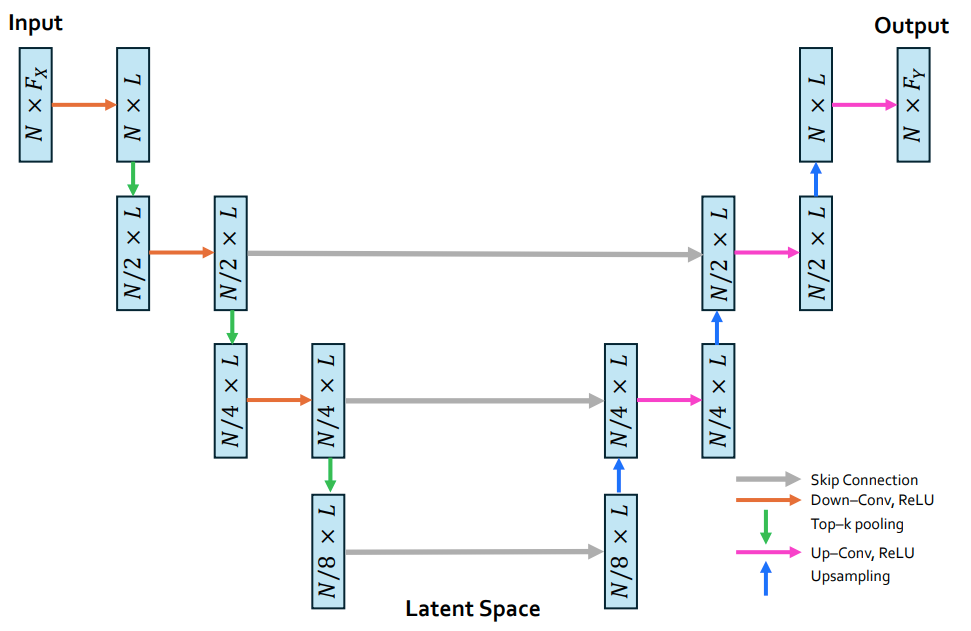
\includegraphics[width=12cm]{images/Methodology/GraphUNet.png}
    \caption{Detailed view of the Graph U-Net architecture applied to fluid dynamics, showcasing an encoder-decoder structure with skip connections. Each layer’s application is annotated with the resultant dimensions, illustrating the feature reduction or expansion throughout the network. Here, L is the number of convolutional layers per convolutional block (channels).}
    % , N is the number of nodes in the graph, and F$_X$ and F$_Y$ denote the number of input and output features respectively.}
    \label{fig:GraphUnet}
\end{figure}
\subsection{Results and discussion}
We develop a surrogate model that uses the exact Graph U-Net architecture. As a first step, we are interested in investigating the ability of the model to reproduce the target data, i.e; when the same target data is given as input. This means that the task solely performs reconstruction of the target dataset, without requiring to predict something. We also go on to perform the prediction task with the same model architecture, which forms the baseline for all the other architectures proposed in this work. The following settings are maintained for both the reconstruction and prediction tasks. We implement a 9-fold cross-validation for the training process. The initial learning rate is set to $0.0005$ and a Step LR scheduler is used to decay the learning rate by a factor of $0.75$ after every 100 epochs. We use the Adam optimizer and train on the RMSE loss for 500 epochs. The model's hyperparameters are selected by a hyperparameter tuning process. Table \ref{table:complex} presents the model complexity and performance on varying the number of channels and hidden layers. It is to be noted that, each hidden layer refers to the combination of sampling (pooling and unpooling) and convolution operations (up and down convolutions). That is, if we perform the pooling and convolutions $d$ times in the encoder and reverse this process $d$ times in the decoder, the number of hidden layers in this architecture is taken as $d$. \\
\begin{table}[ht]
    \centering
    \caption{Hyperparameter tuning - Table depicting the number of channels, hidden layers, trainable parameters, training loss, and validation loss, measured with the RMSE criterion, for the Baseline architecture corresponding to each setting.}
    \label{table:complex}
    \begin{tabular}{|c|c|c|c|c|}
    \hline
    \textbf{Channels} & \textbf{Hidden layers} & \textbf{Trainable parameters} & \textbf{Training loss} & \textbf{Validation loss}\\
    \hline
    \multirow{4}{*}{48} & 2 & 7k &  0.04876&  0.05166\\
    \cline{2-5}
                        & 3 & 12k &  0.04713&  0.05128\\
    \cline{2-5}
                        & \textbf{4} & \textbf{17k} & \textbf{0.04386}&  \textbf{0.05237}\\
    \cline{2-5}
                        & 5 & 22k &  0.04272 &  0.05299\\
    \hline
    \multirow{4}{*}{64} & 2 & 13k & 0.04536&  0.05349\\
    \cline{2-5}
                        & 3 & 21k & 0.05074 &  0.05472\\
    \cline{2-5}
                        & 4 & 30k &  0.04139&  0.05615\\
    \cline{2-5}
                        & 5 & 31k & 0.04692 &  0.05587\\
    \hline
    \multirow{4}{*}{128} & 2 & 51k& 0.03983&  0.05639\\
    \cline{2-5}         
                         & 3 & 84k & 0.03840&  0.05492\\
    \cline{2-5}
                         & 4 & 117k & 0.03642 &  0.05341 \\
    \cline{2-5}
                         & 5 & 150k &  0.05011&  0.05563\\
    \hline
    \end{tabular}
    
    \end{table}
Out of the various architectures, we select the model that gives the lowest training loss and validation loss, or one that offers a good compromise between the two losses. Among the models with similar performance, we choose the one that is the simplest, i.e; has relatively lesser trainable parameters, without compromising on the accuracy or facing the risk of overfitting. Hence, we execute the training process using a GNN architecture with 48 channels and carry out the sampling and convolution operations 4 times (number of hidden layers) on the encoder and the decoder side. Similar experiments have been conducted to choose the ideal batch size, activation function and other hyperparameters. The key hyperparameters are listed in Table \ref{table:hp}. 
\begin{table}[ht]
    \centering
    \caption{Model hyperparameters}
    \label{table:hp}
    \begin{tabular}{|l|l|}
    \hline
    \textbf{Hyperparameter}    & \textbf{Value/Description} \\
    \hline
    Channels    & 48                           \\
    \hline
    Hidden layers    & 4                          \\
    \hline
    Pooling ratios             & [0.5,0.5,0.5,0.5]                       \\
    \hline
    Batch size                 & 4                         \\
    \hline
    Activation function        & ReLU                       \\
    \hline
    Weight initialization    &  Kaiming                        \\
    \hline
    Initial learning rate       & 0.0005                       \\
    \hline
    \end{tabular}
    \end{table}
\subsubsection{Reconstruction task}
As mentioned previously, we prescribe the same steady-state CFD dataset as the input and target data to evaluate the effectiveness of reconstruction of the Graph U-Net model. The CFD results, predictions of the GNN model and the absolute difference between them for four simulation cases from the test dataset are shown in Figure \ref{blrecon}.\\
\begin{figure}[ht]
    \centering
    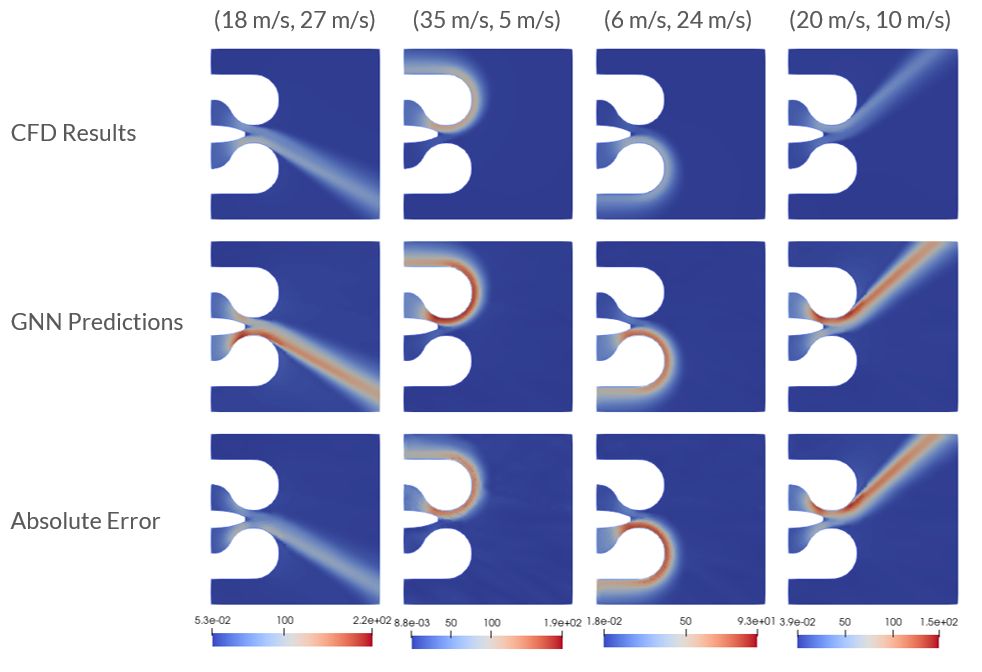
\includegraphics[width=14cm]{images/Methodology/allvelrecon.png}
    \caption{Visualization of velocity fields for four cases from the baseline's reconstruction task, with inlet velocity values prescribed as (Inlet 1, Inlet 2). Here, the first row represents the target data, the second row corresponds to the model predictions, and the last row is the absolute difference between them. The colours signify the magnitude of velocity, mapped by the legend.} 
    \label{blrecon}
\end{figure}
Although the model reconstructs the trends of the outflow jet similar to the target data, the scale or the range of velocity magnitude is slightly different for the two cases. The pressure field, though not depicted here, also faces the same problem. Thus, the baseline model fails to accurately capture the steady state fields during reconstruction. The lack of explicit unpooling layers in Graph U-Net can be attributed as the cause of inadequate reconstruction of the original graph structure during decoding. 
\subsubsection{Prediction task}
In this case, we predict the steady-state solutions from the earlier transition state. The CFD results, predictions of the GNN model and the absolute difference between these data for four simulation cases from the test dataset are shown in Figure \ref{blpred}.
\begin{figure}[ht]
    \centering
    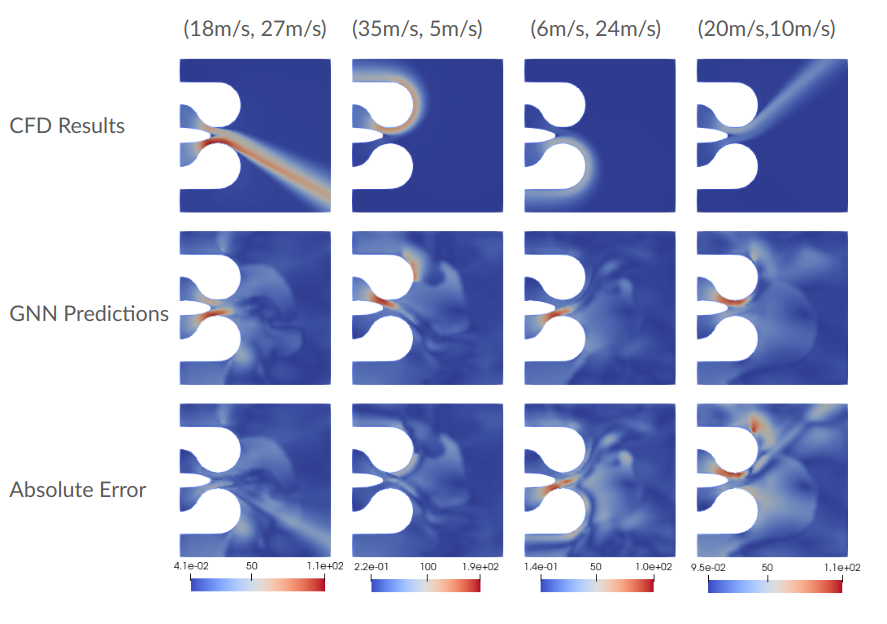
\includegraphics[width=14cm]{images/Methodology/Baselineprediction.png}
    \caption{Visualization of velocity fields for four cases from the baseline's prediction task, with inlet velocity values prescribed as (Inlet 1, Inlet 2) presented in four columns. Here, the first row represents results the target data, the second row corresponds to the GNN predictions for the velocity field, and the last row is the absolute difference between the target data and GNN predictions. The colours signify the magnitude of velocity, mapped by the legend.} 
    \label{blpred}
\end{figure}
As we can understand from the figure, the behavior of the outflow jet as well as its magnitude vary significantly from the expected target data. Thus, the baseline model is not feasible for the prediction task of nozzle flow dynamics. To better comprehend and evaluate the model performance, we estimate the training, validation and test losses of the baseline model for both the tasks in Table \ref{table:perform}. We also note down the absolute difference between the input and target data for the test dataset of the prediction task.  
\begin{table}[ht]
    \centering
    \caption{Model evaluation metrics of the Baseline model for the reconstruction and prediction tasks.} 
    \label{table:perform}
    \begin{tabular}{|l|l|l|l|l|}
    \hline
    \textbf{Model} & \textbf{Training Loss} & \textbf{Validation Loss} & \textbf{Test Loss} & \textbf{Abs Difference} \\
    \hline
    Baseline - Reconstruction & 0.025627 & 0.028391 & 0.029312 & 0\\
    \hline
    Baseline - Prediction & 0.1459 & 0.1503 & 0.1635 & 0.2626\\
    \hline
    \end{tabular}
    \end{table}   
\subsection{Limitations}
As observed in the previous section, Graph U-Nets are not suitable for predicting steady-state solutions. Originally designed for small graphs with around 100 nodes, Graph U-Net relies on dense matrix multiplications, which are memory-intensive and not scalable. This leads to memory constraints and slower training times, thus making it impractical for complex, large-scale graph data. GCNConv layers used in this architecture may have limited expressiveness in capturing higher-order graph structures and capturing long-range dependencies in the graph. Its optimal depth is found to be 2 or 3 layers \cite{kipf}. Deeper models beyond 7 layers can encounter training difficulties from risk of overfitting. Apart from these issues, there is also a lack of a dedicated upsampling layer in the architecture which leads to poor reconstruction of the latent space. Due to these disadvantages, Graph U-Net may exhibit poor performance in terms of both accuracy and efficiency, particularly for complex geometries or large datasets. Hence, there is a paramount necessity to rely on modified GNN architectures for our work.
\section{Proposed architecture}
\label{proparch}
In this section, we propose three GNN surrogate models and elucidate the architecture and improvements made on the original Graph U-Net framework. Then, we proceed to provide details on the hyperparameters and other implementation specifics of the proposed models. Finally, we demonstrate the training process and share the predictions results obtained for the CFD application. The models are developed on the Pytorch deep learning framework using the Pytorch Geometric (PyG) library. Training and testing are performed on a compute node of the \gls{HPC} cluster Loewenburg, using a single nVidia Tesla V100 GPU. \\
There are 3 different surrogate models proposed and each of them tackle the unpooling limitation in Graph U-Net by using a \gls{k-NN} approach for upsampling used in PointNet++ \cite{pnpp}, with k set to 3. The downsampled features at different depths (levels of coarsening) are stored so that the upsampled node co-ordinates required for k-NN interpolation can be obtained from $[c_{x}, c_{y}]$ at the downsampled feature of the same depth. The architectures also include skip connections, although they do not perform the task of upsampling here. The three surrogate models differ in the convolutional operations used, as described below. 
\begin{enumerate}
    \item \textit{Graphknn} uses GCNConv layers as used in Graph U-Nets to perform convolutions and executes the upsampling operation with the help of k-NN interpolation. 
    \item The \textit{SAGEknn} surrogate model replaces the GCNConv layers of Graph U-Net with SAGEConv layers from GraphSAGE \cite{SAGE} and uses k-NN interpolation for unpooling. 
    \item In \textit{MoNetknn}, we carry out convolutions using the GMMConv layers from the MoNet \cite{MoNet} architecture along with k-NN interpolation for upsampling. 

    % \item \textit{BL + crsn + knn:} In this surrogate, we first obtain the set of coarsened meshes through incremental decimation of the CFD mesh by running a Python script on Paraview. With the mesh indices and co-ordinates of the low-resolution mesh nodes, we compute the downsampled features for the graph using the sampling operator described in the subsection \ref{SO}. Thus, we implement the pooling operation with the help of sampling operator and perform unpooling operation using k-NN interpolation. 
    % \item \textit{BL + SAGE + crsn + knn:} Similar to the previous model in every detail, the only difference in this model is that it uses GraphSAGE layers instead of the GCNConv layers as convolutions.
    % \item \textit{BL + MoNet + sampl. + knn:} This model is also similar to \textit{BL + crsn + knn}, but it applies MoNet blocks for up convolutions and down convolutions. 
\end{enumerate}
We perform hyperparameter tuning for each of the architectures to arrive at the ideal choice of design parameters. All the models showcase their best performance for the same hyperparameter configuration - 48 channels, 3 hidden layers each with a pooling ratio of 0.5, ReLU activations and weights initialized by the Kaiming method. We use a batch size of 4 and set up the initial learning rate as 0.0005, to be used along with a Step LR scheduler similar to the baseline surrogates. We use the Adam optimizer and train on the RMSE loss. 


% The salient features of the three architectures along with their hyperparameters are tabulated in Table \ref{prophp}. 
% % \subsection{Multi-Resolution Graph Net Architecture}
% % \section{Model hyperparameters and training parameters}
% \begin{table}[ht]
%     \centering
%     \caption{Features and hyperparameters comparison of 1. \textit{Graphknn}, 2. \textit{SAGEknn}, and 3. \textit{MoNetknn} architectures.}
%     \label{prophp}
%     \begin{tabular}{|l|l|l|l|}
%     \hline
%     \textbf{Feature/Hyperparameter}    & \textit{Graphknn} & \textit{SAGEknn}   & \textit{MoNetknn} \\
%     \hline
%     Channels    & 48 & 48 & 48                           \\
%     \hline
%     Hidden layers    & 3 & 3 & 3                          \\
%     \hline
%     Convolution layer             &     GCNConv & SAGEConv & GMMConv                   \\
%     \hline
%     Pooling operation             &    Top-k &  Top-k &  Top-k                     \\
%     \hline
%     Unpooling operation         &   k-NN&   k-NN &   k-NN               \\
%     \hline
%     Batch size                 & 4 & 4& 4                         \\
%     \hline
%     Activation function        & ReLU  & ReLU  & ReLU                       \\
%     \hline
%     Weight initialization    &  Kaiming &  Kaiming &  Kaiming                        \\
%     \hline
%     Initial learning rate       & 0.0005 & 0.0005 & 0.001                        \\
%     \hline
%     \end{tabular}
%     \end{table}
\section{Results and discussion}
We perform a 9-fold cross-validation on the training and validation datasets. Figures \ref{2vel1} and \ref{2vel2} depict the predicted velocity fields and the associated absolute errors obtained from the three surrogates for four different flow conditions. Figure \ref{aloop} provides an overview of the predicted pressure and velocity fields for all the surrogate models discussed here for a case showing Coanda adhesion. \\
\begin{figure}[ht]
    \centering
    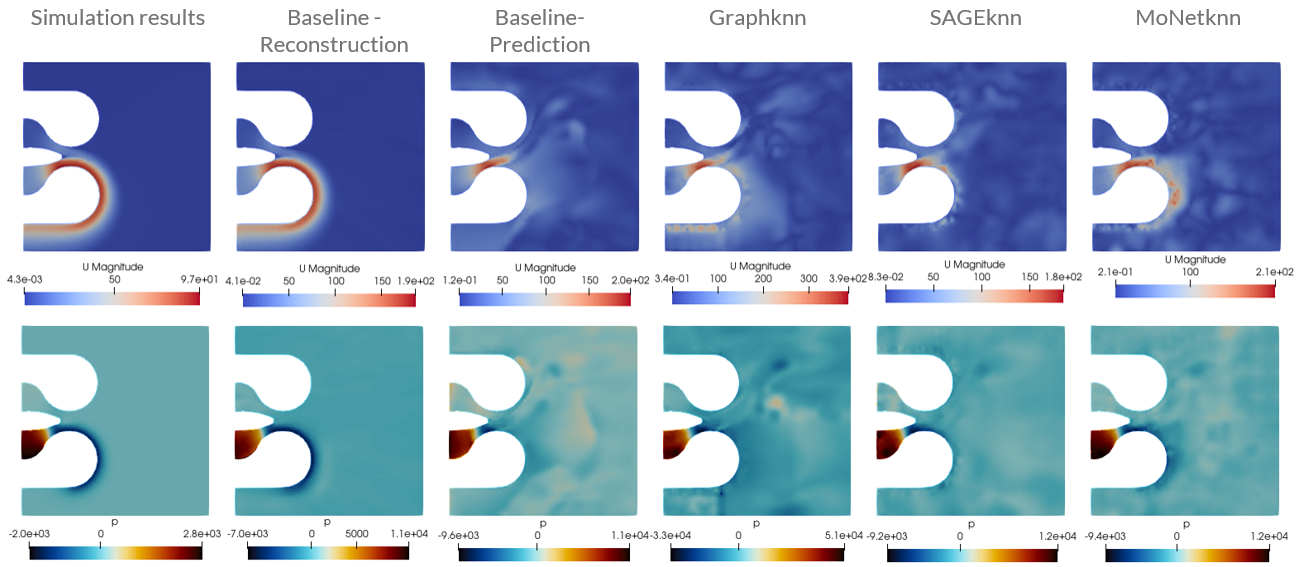
\includegraphics[width=16cm]{images/Methodology/presvelcomp.png}
    \caption{Predicted velocity and pressure fields for the case with (Inlet 1, Inlet 2) = (35 m/s, 5 m/s). The leftmost column represents simulation results whereas every other column corresponds to the predictions of the respective architectures.} 
    \label{aloop}
\end{figure}
\begin{figure}[ht]
    \centering
    \begin{subfigure}[b]{14cm}
        \centering
        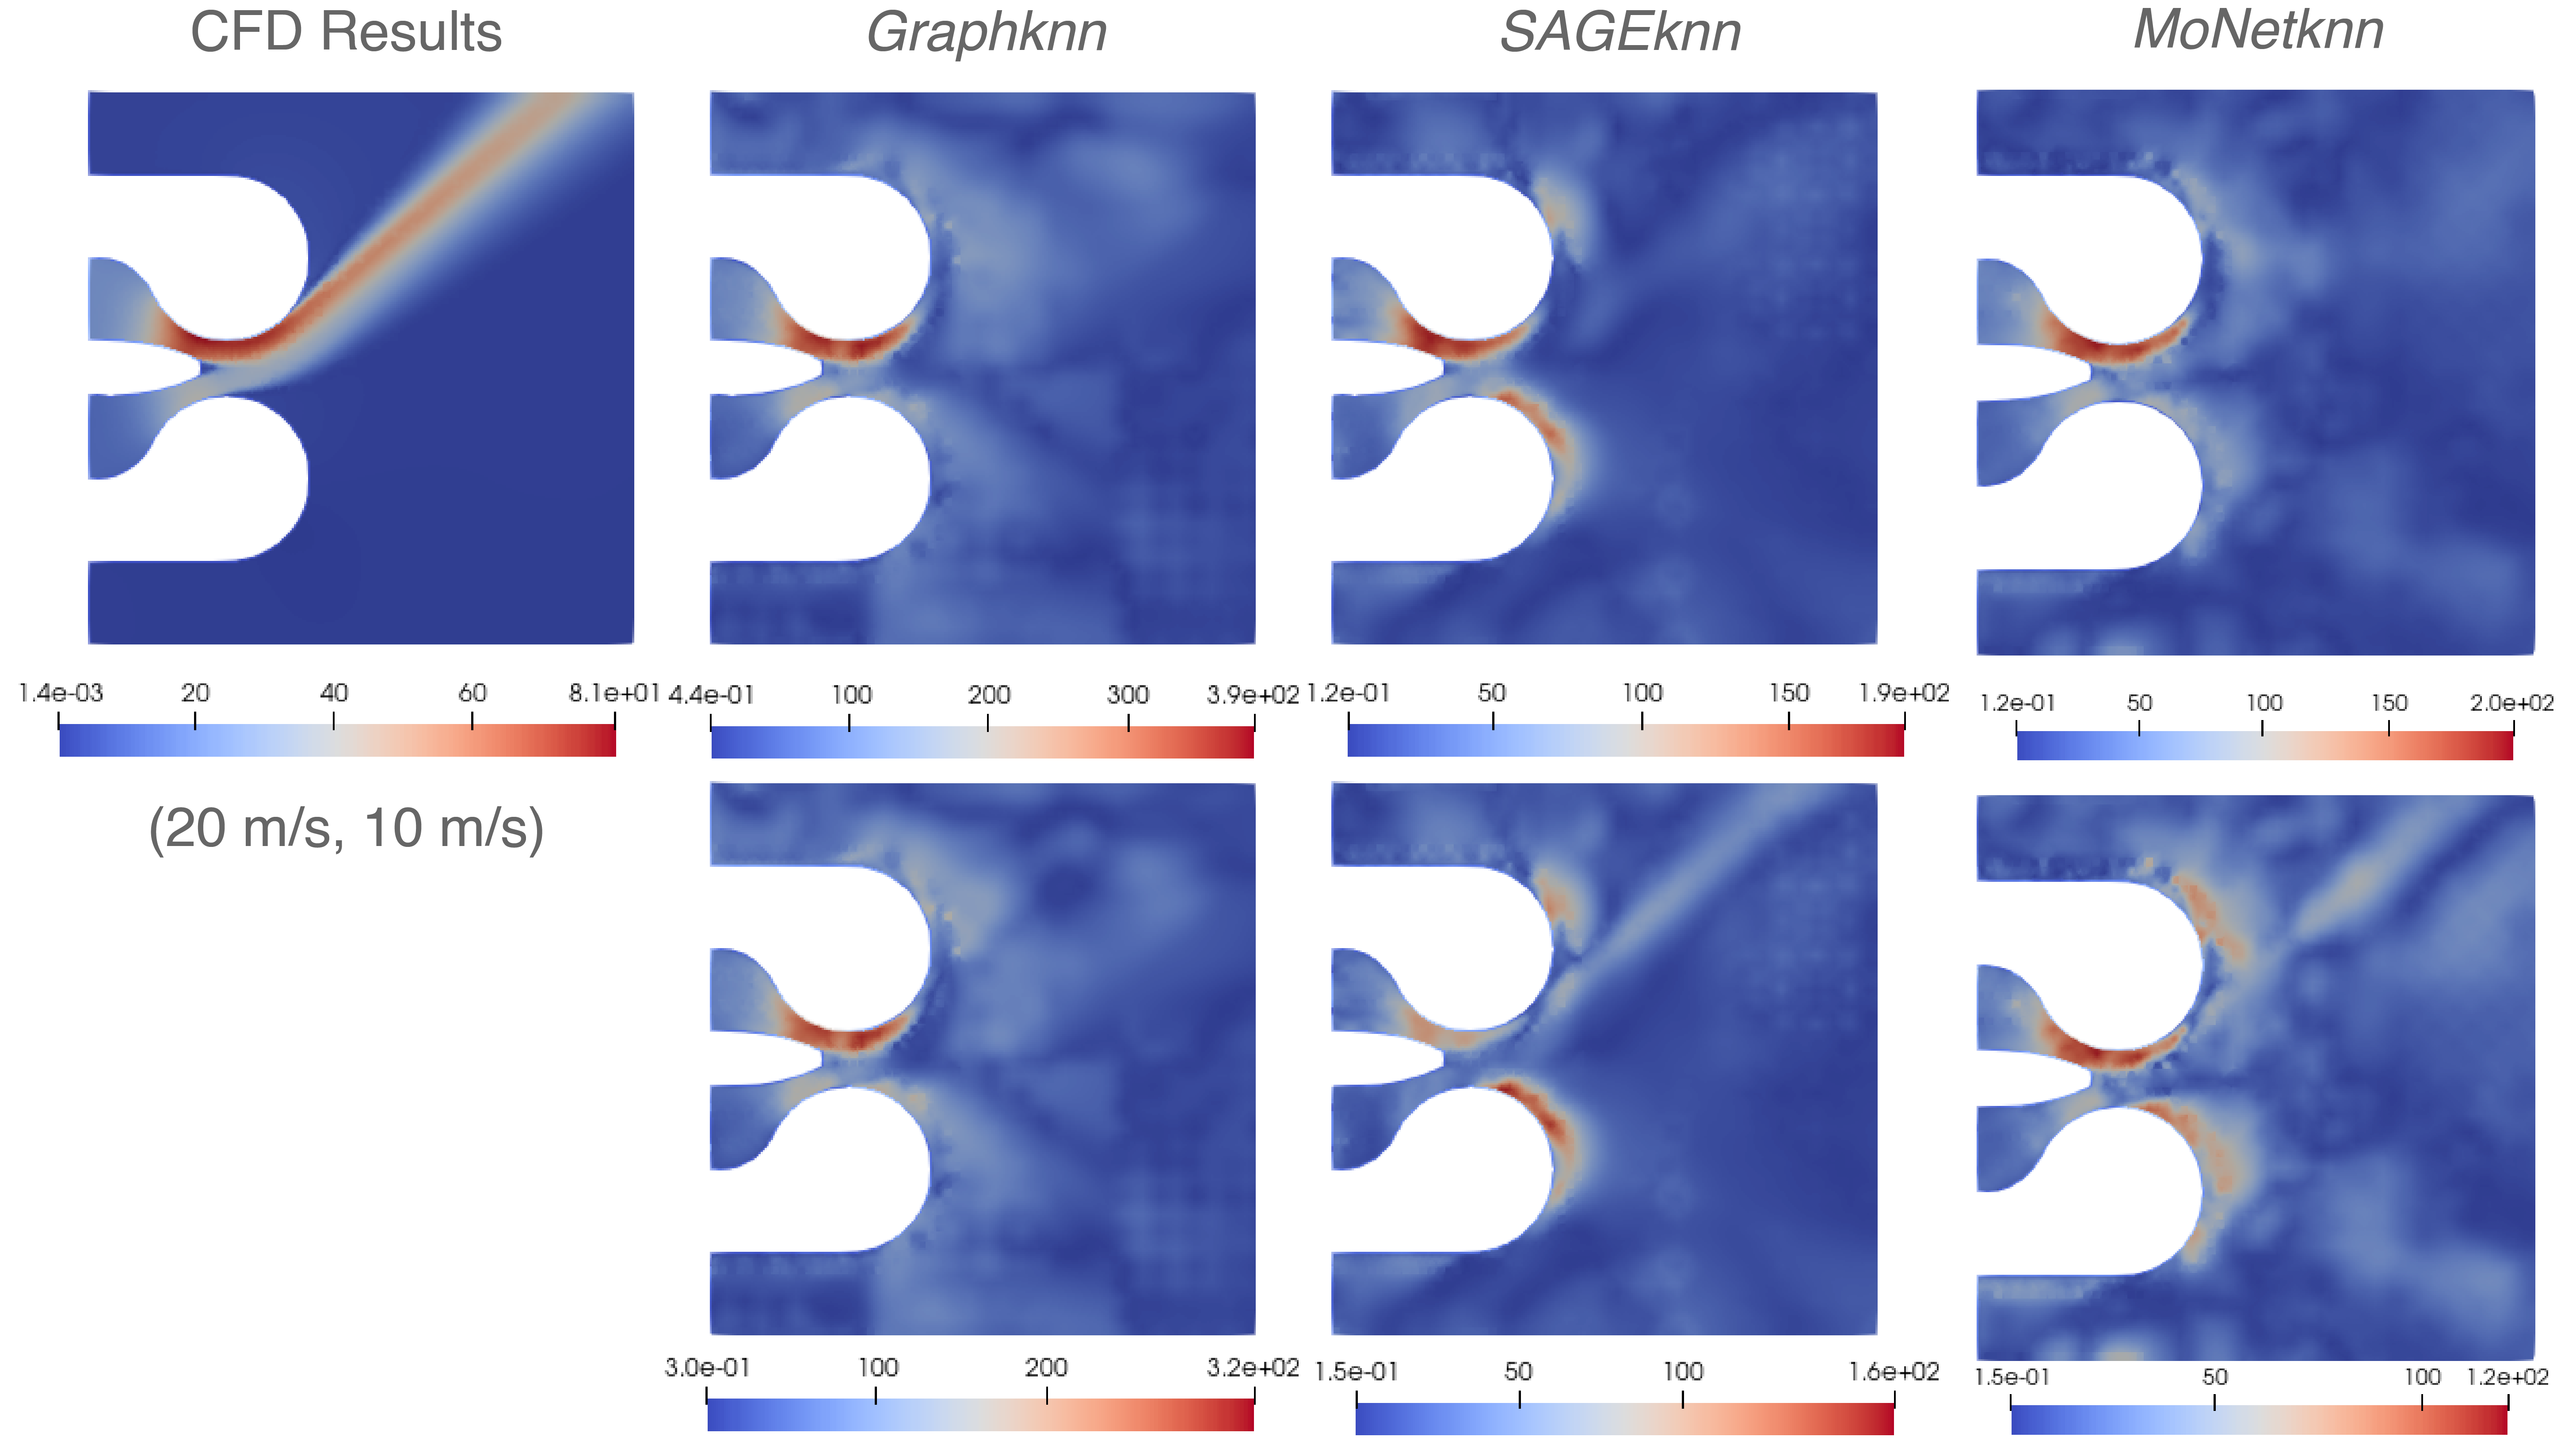
\includegraphics[width=\textwidth]{images/Methodology/Asset 18.png}
        \caption{Case (20 m/s, 10 m/s) showing jet deflection to the top Coanda surface.}
        \label{fig:allvel1}
    \end{subfigure}
    % \vspace{2.5cm} % Adds some vertical space between the subfigures
    \begin{subfigure}[b]{14cm}
        \centering
        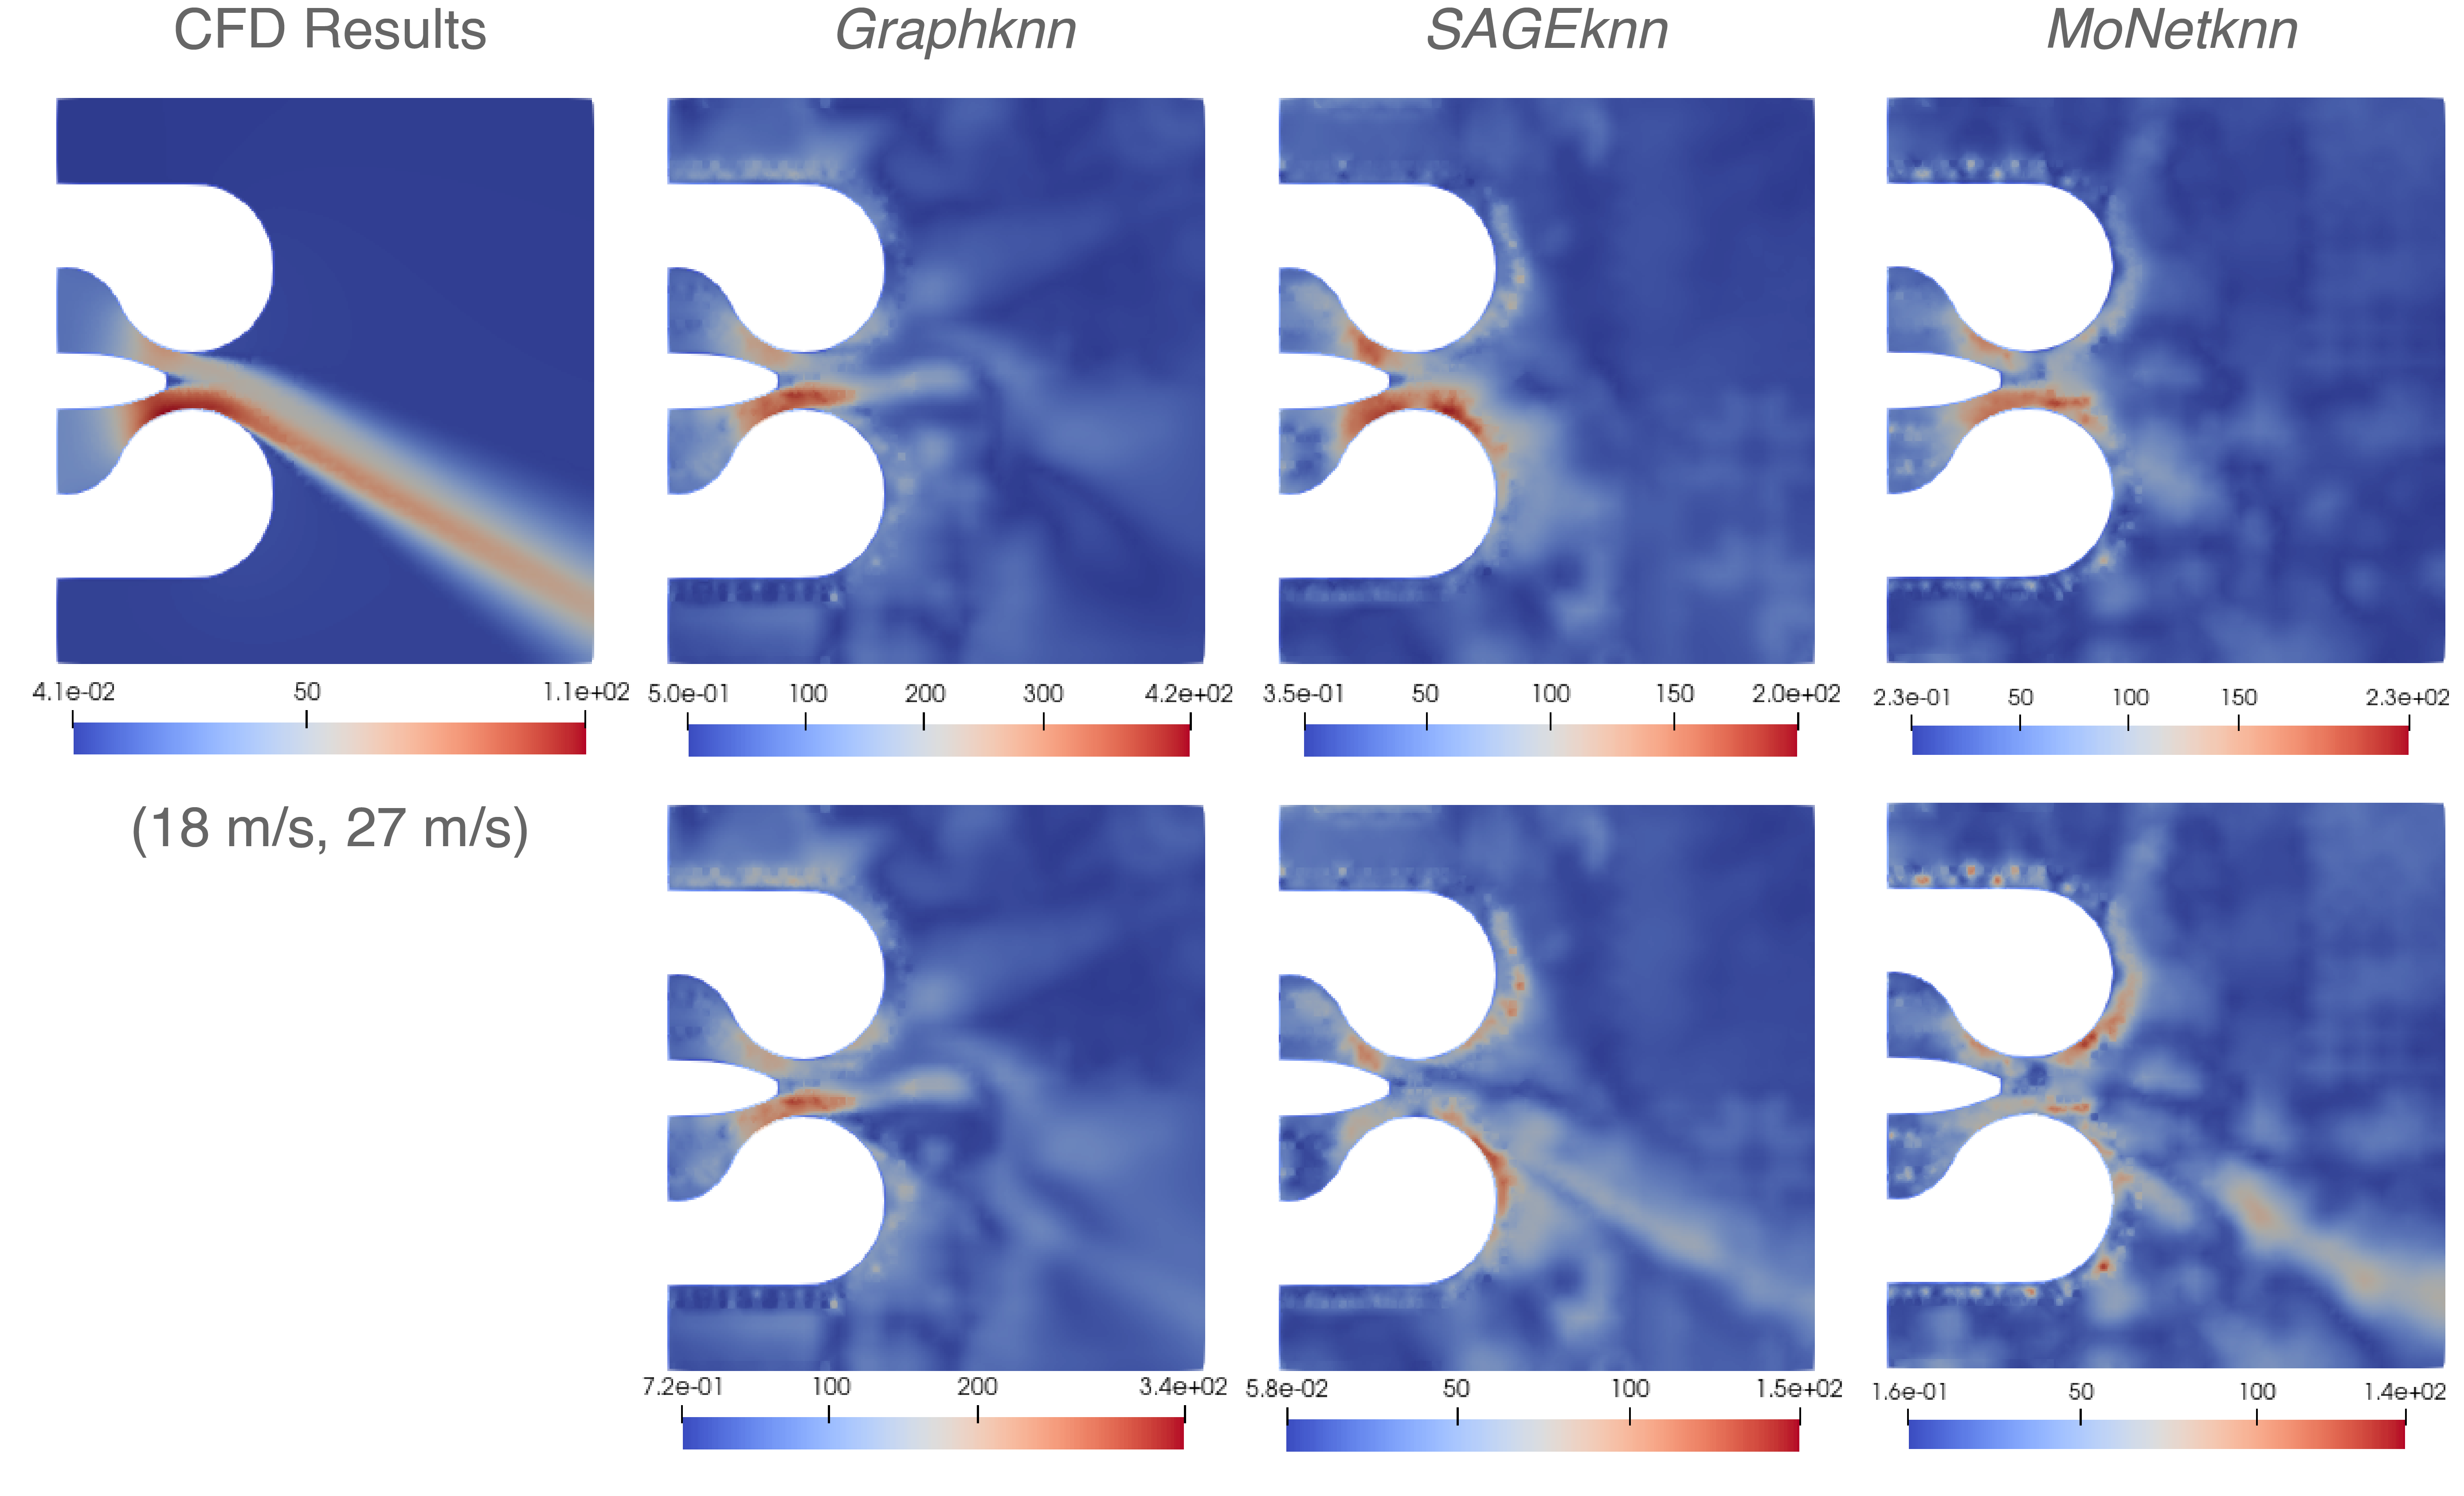
\includegraphics[width=\textwidth]{images/Methodology/Asset 17.png}
        \caption{Case (18 m/s, 27 m/s) showing jet deflection to the bottom Coanda surface.}
        \label{fig:allvel2}
    \end{subfigure}
    % \vspace{-10mm} % Adds some vertical space between the subfigures
    \caption{Visualization of velocity fields for two cases with inlet velocities (Inlet 1, Inlet 2): the first row depicts the predictions and the second row shows the absolute difference between the target and predictions. The top left corner presents the simulation results.}
    \label{2vel1}
\end{figure}
\begin{figure}[ht]
    \centering
    \begin{subfigure}[b]{14cm}
        \centering
        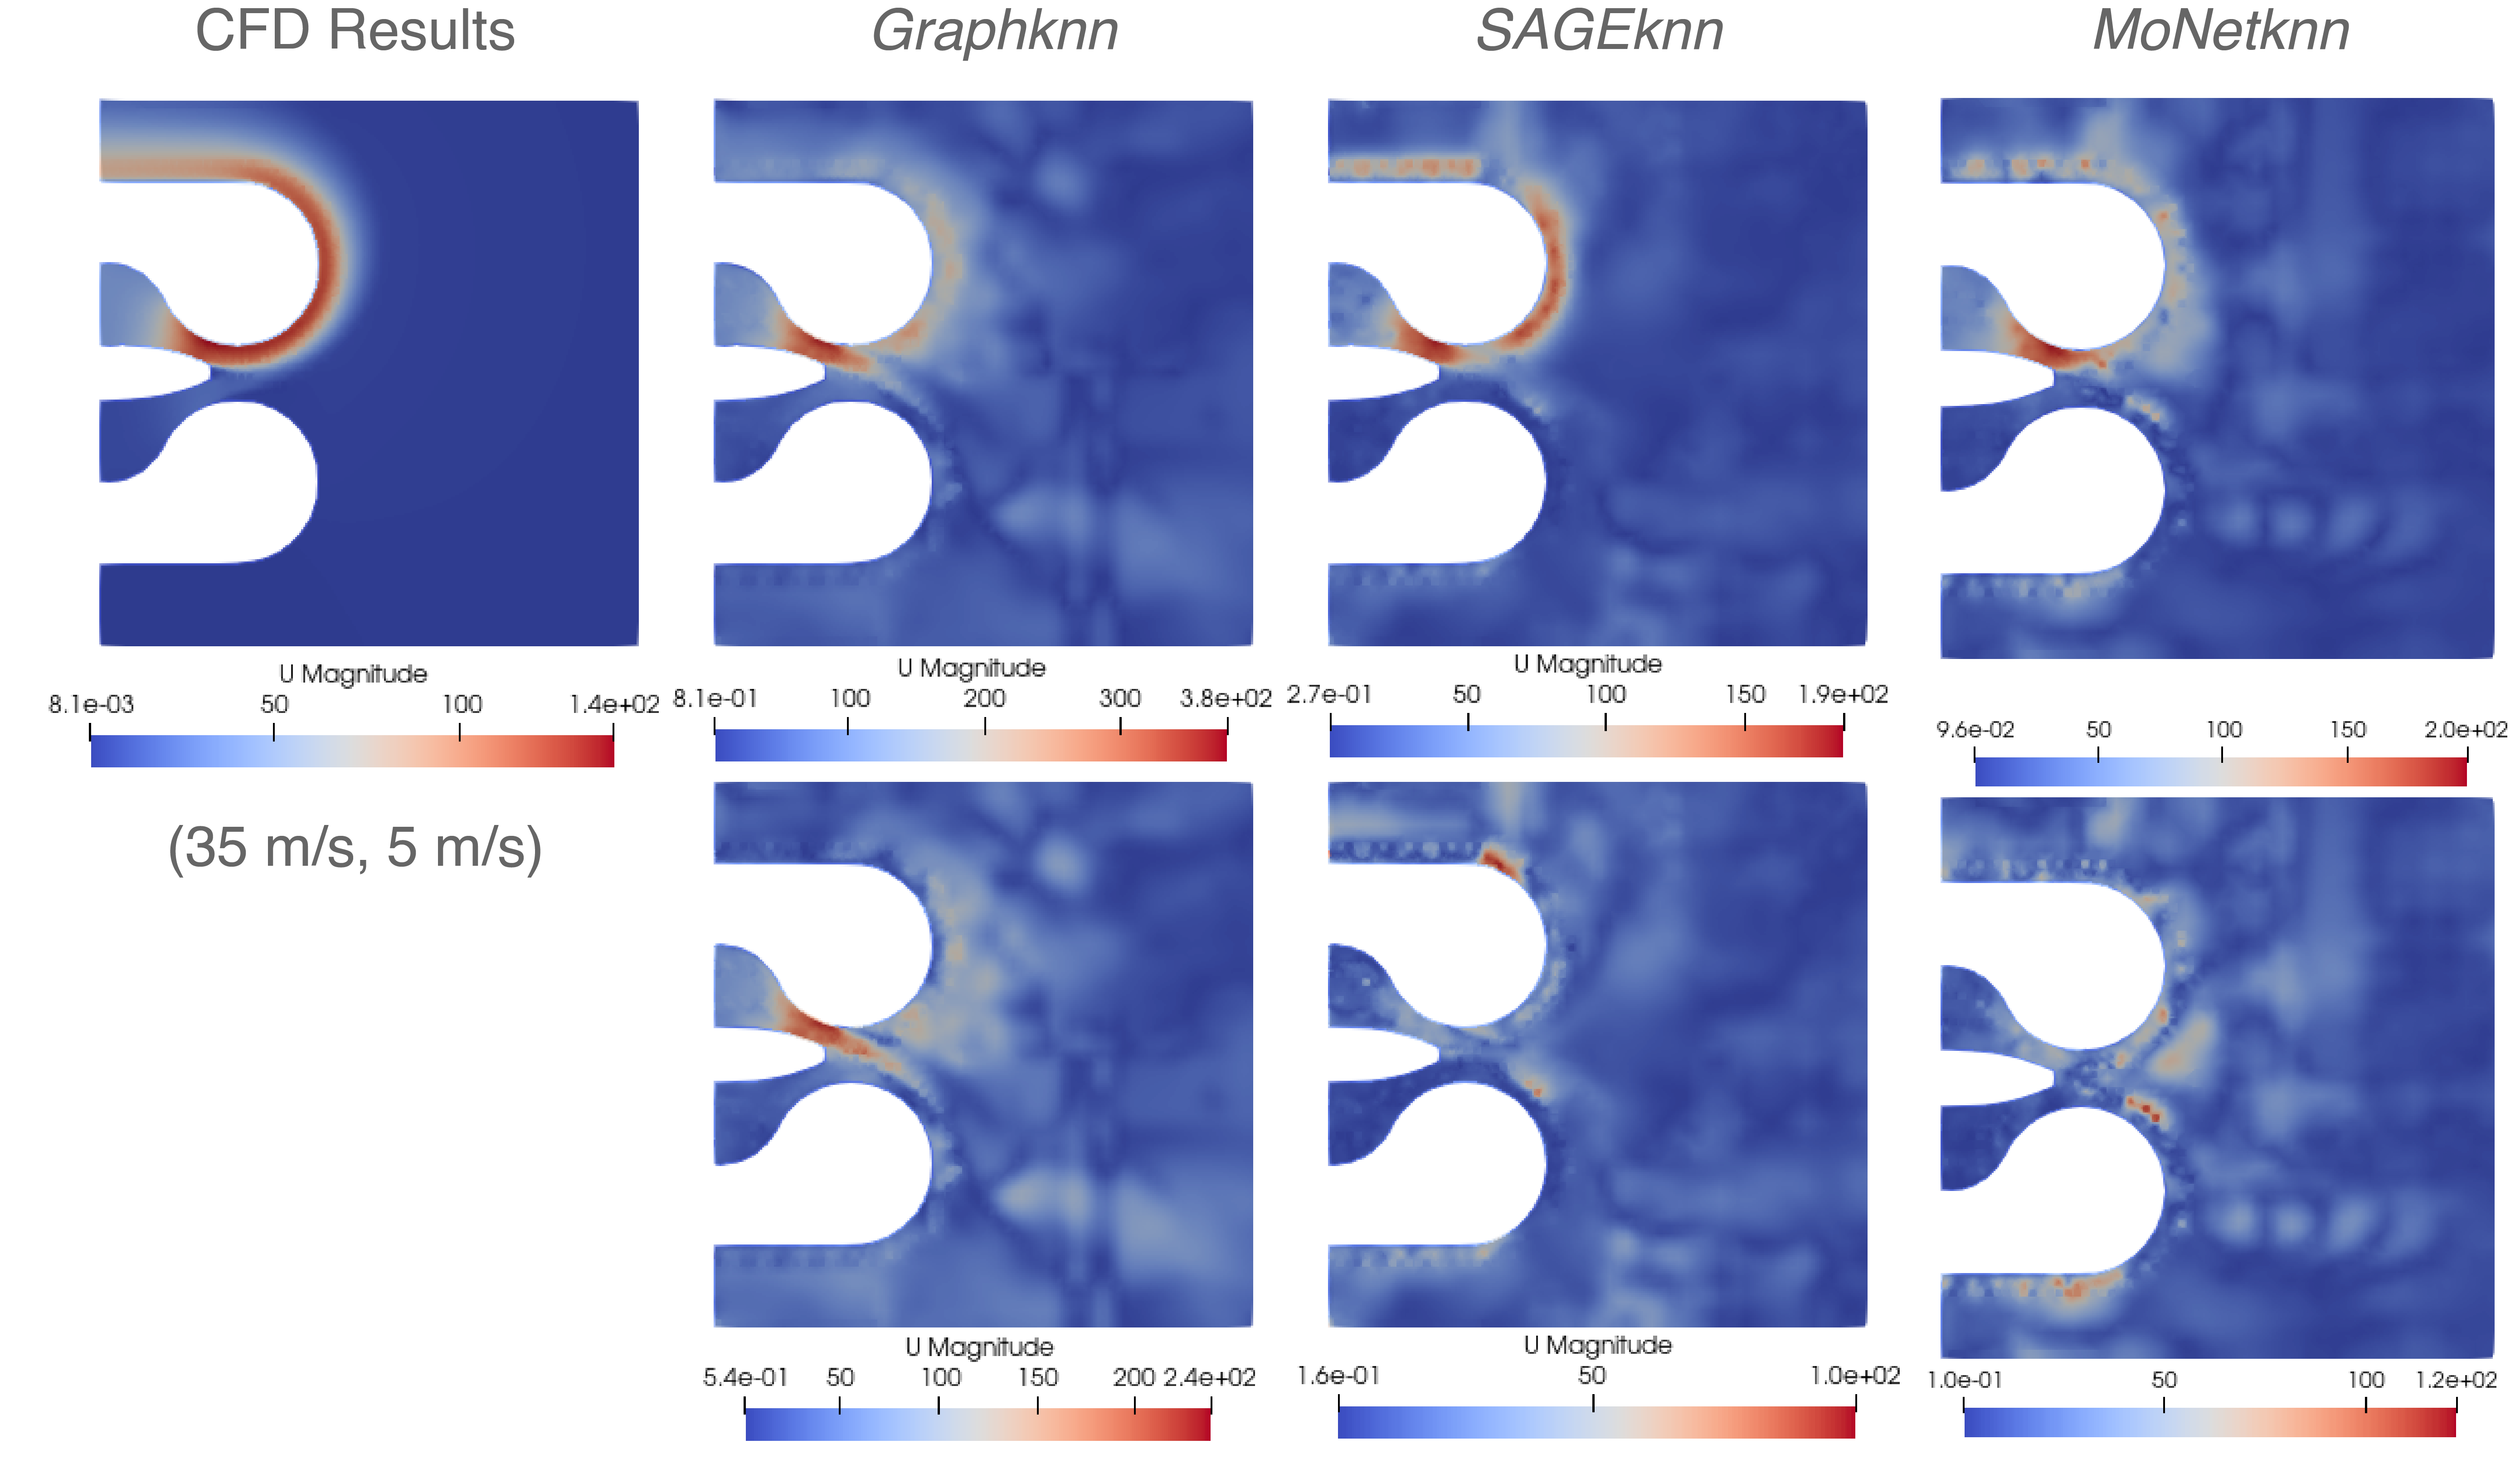
\includegraphics[width=\textwidth]{images/Methodology/Asset 15.png}
        \caption{Case (35 m/s, 5 m/s) showing complete adhesion to the top Coanda surface.}
        \label{fig:allvel3}
    \end{subfigure}
    % \vspace{2.5cm} % Adds some vertical space between the subfigures
    \begin{subfigure}[b]{14cm}
        \centering
        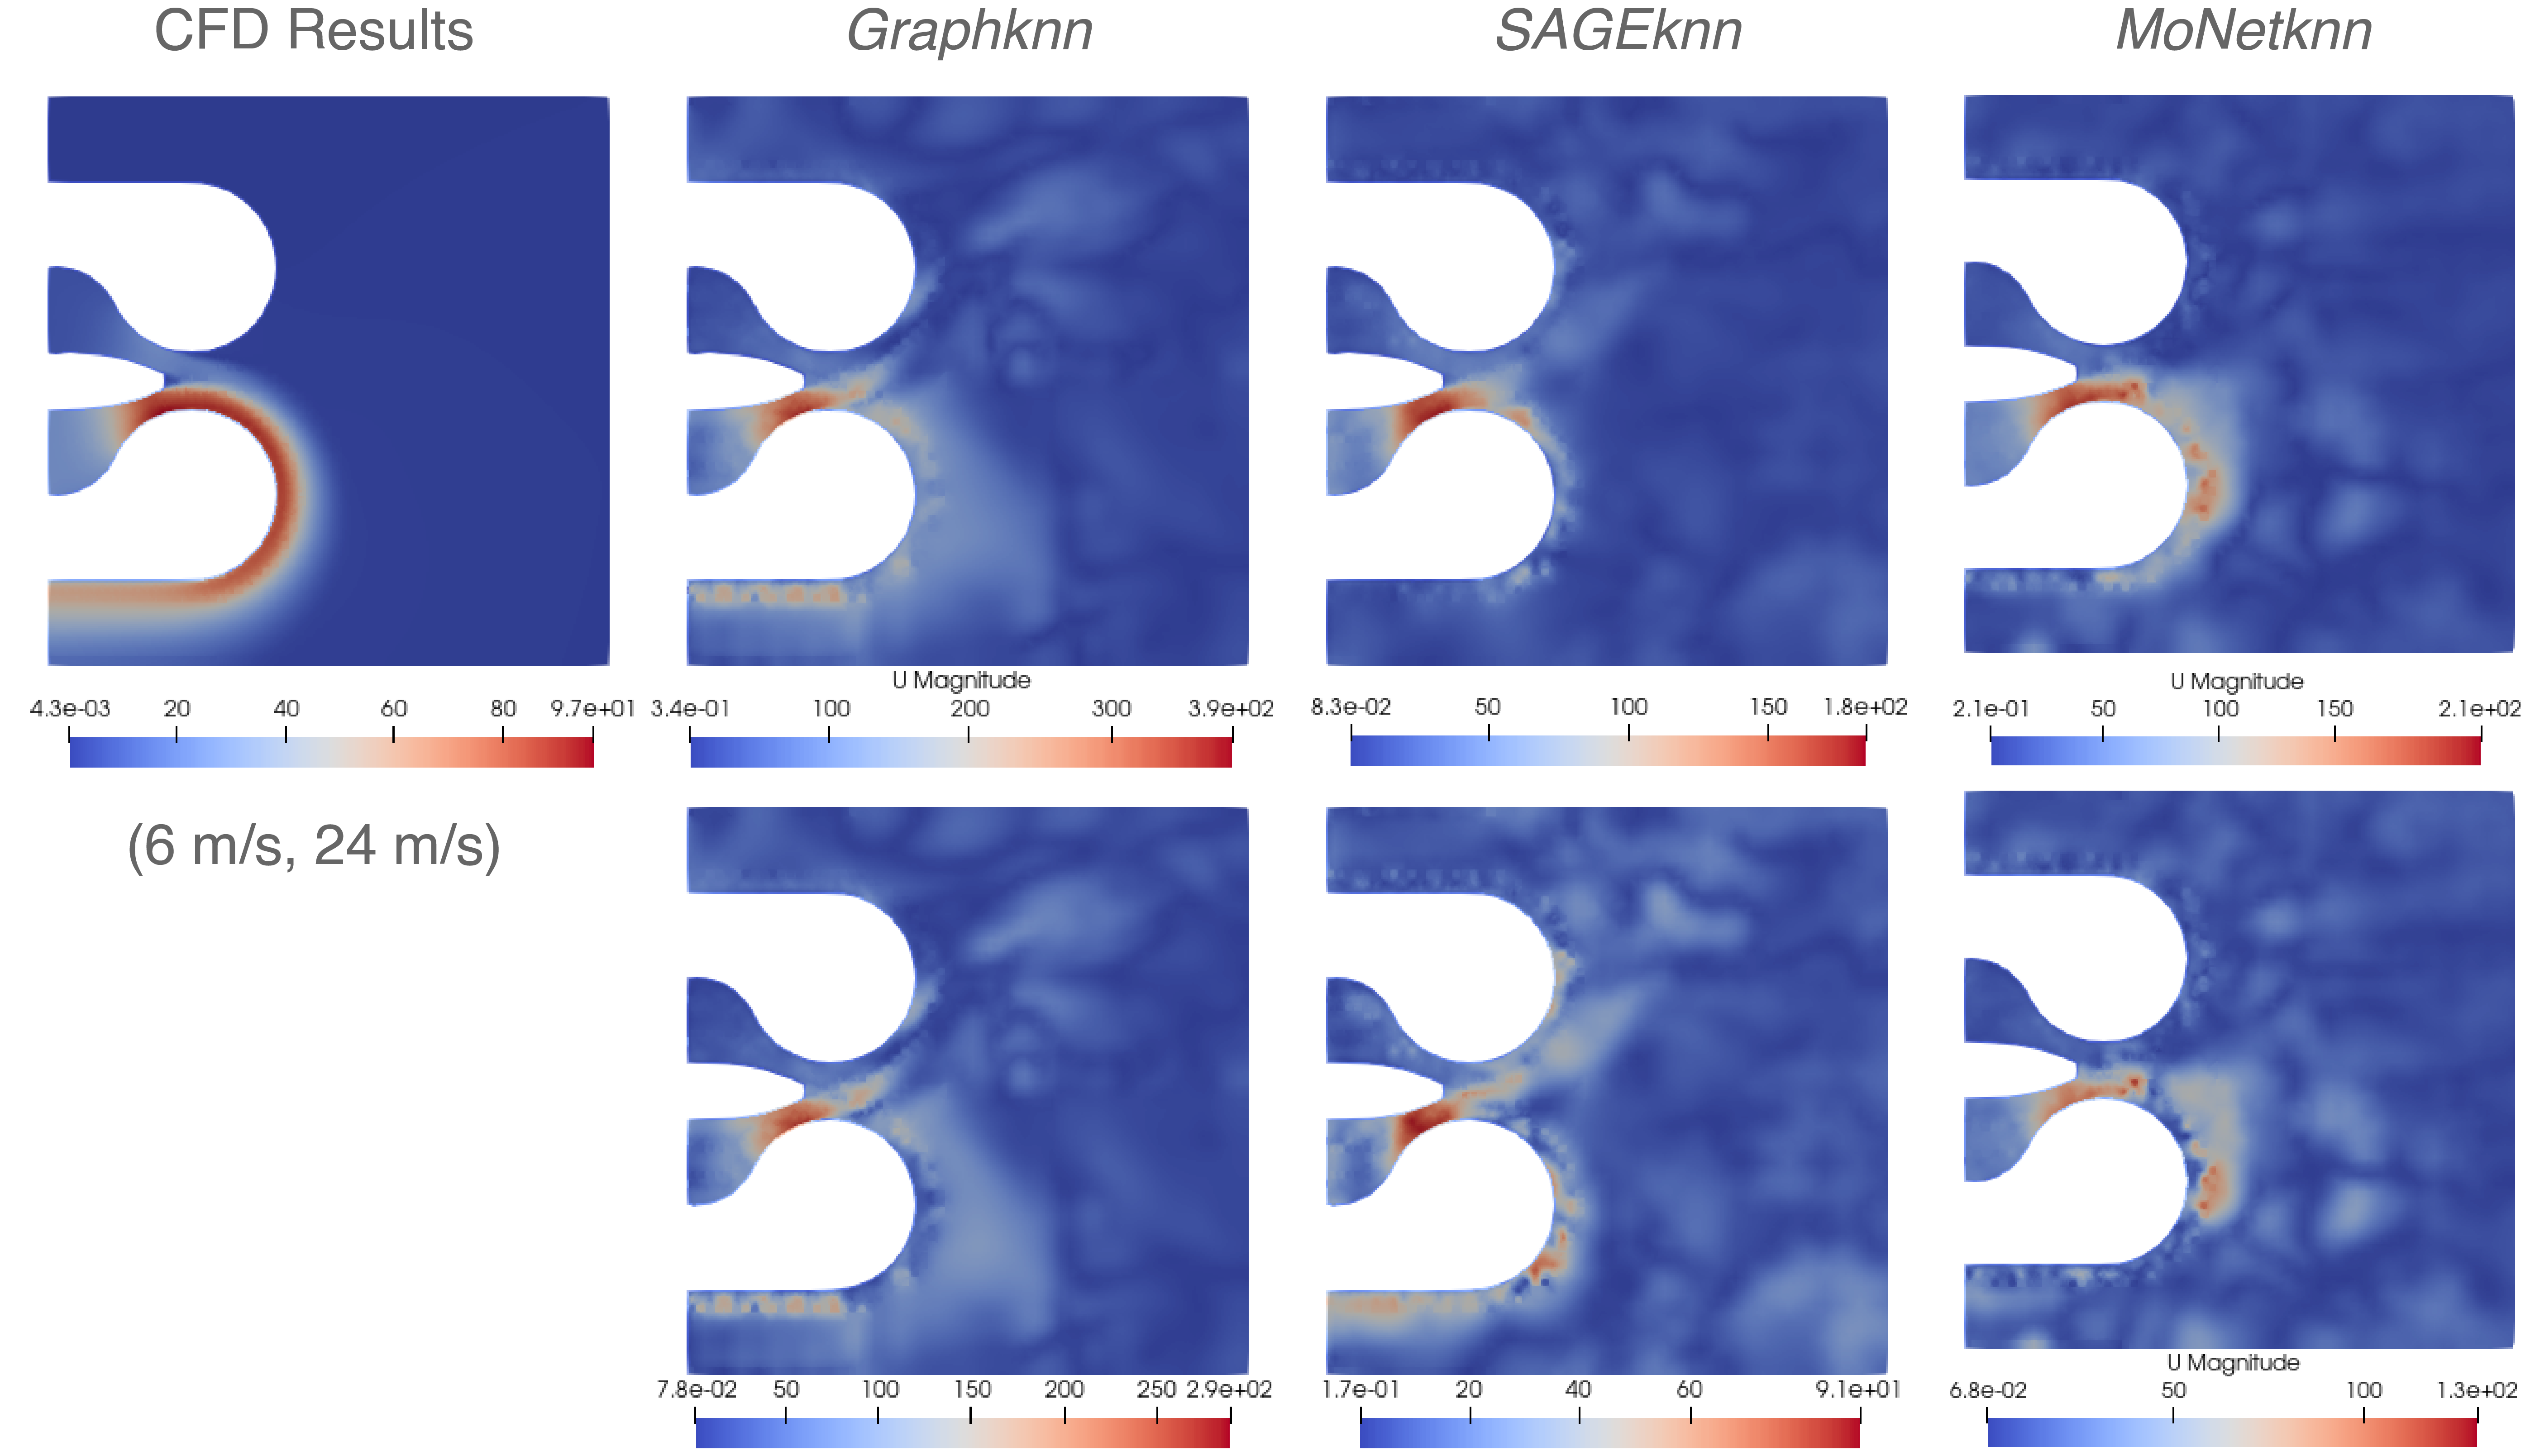
\includegraphics[width=\textwidth]{images/Methodology/Asset 14.png}
        \caption{Case (6 m/s, 24 m/s) showing complete adhesion to the bottom Coanda surface.}
        \label{fig:allvel4}
    \end{subfigure}
    % \vspace{-10mm} % Adds some vertical space between the subfigures
    \caption{Visualization of velocity fields for two cases with inlet velocities (Inlet 1, Inlet 2): the first row depicts the predictions and the second row shows the absolute difference between the target and predictions. The top left corner presents the simulation results.}
    \label{2vel2}
\end{figure}
To discern the performance of these models, we compute the RMSE loss over the training, validation and test datasets, observed in Table \ref{t:predloss}. We observe that the \textit{MoNetknn} architecture performs slightly better than \textit{SAGEknn} which is marginally superior to \textit{Graphknn} in terms of training loss. While \textit{Graphknn} surpasses the other two models in terms of test loss, \textit{SAGEknn} proves to be the relatively better model to \textit{MoNetknn} on the test dataset. Furthermore, we also monitor the training and test times of the three models along with the time taken to batch execute the CFD simulations, presented in Table \ref{t:times}. 
\begin{table}[ht]
    \centering
    \caption{Evaluation metrics of  1. \textit{Graphknn}, 2. \textit{SAGEknn}, and 3. \textit{MoNetknn} architectures. } 
    \label{t:predloss}
    \begin{tabular}{|l|l|l|l|}
    \hline
    \textbf{Model} & \textbf{Training Loss} & \textbf{Validation Loss} & \textbf{Test Loss}\\
    \hline
     \textit{Graphknn} & 0.134412& 0.143149 & 0.143952   \\
    \hline
    \textit{SAGEknn}& 0.123704 & 0.138665 & 0.149408 \\
    \hline
    \textit{MoNetknn} & 0.110712  & 0.143189& 0.15305  \\
    \hline
    \end{tabular}
\end{table}
% \begin{table}[ht]
%     \centering
%     \caption{Time taken for training and testing of  1. \textit{Graphknn}, 2. \textit{SAGEknn}, 3. \textit{MoNetknn} models, 4. Transition, and 5. Steady-state simulations.} 
%     \label{t:times}
%     \begin{tabular}{|l|l|l|l|l|l|}
%     \hline
%     \textbf{Model} & \textit{Graphknn} & \textit{SAGEknn} & \textit{MoNetknn} & Transition & Steady-state \\
%     \hline
%     Training time (hours) & 3.88 & 3.2& 4.15  & 8.5 & 0.3 \\
%     \hline
%     Test time (seconds) & 0.09157  & 0.09382 & 0.09413 & -& - \\
%     \hline
%     \end{tabular}
% \end{table}
\begin{table}[ht]
    \centering
    \caption{Time taken for training and testing of  (1) \textit{Graphknn}, (2) \textit{SAGEknn}, (3) \textit{MoNetknn} models, (4) Transition, and (5) Steady-state simulations. Note that training time for (4) and (5) refers to simulation times.} 
    \label{t:times}
    \begin{tabular}{|l|l|l|}
    \hline
    & \textbf{Training time (hours)} & \textbf{Test time (seconds)} \\
    \hline
    \textit{Graphknn} & 3.88 & 0.09157 \\
    \hline
    \textit{SAGEknn} & 3.2 & 0.09382 \\
    \hline
    \textit{MoNetknn} & 4.15 & 0.09413 \\
    \hline
    Steady-state& 8.5 & - \\
    \hline
    Transition & 0.3 & - \\
    \hline
    \end{tabular}
\end{table}
The duration of steady-state simulations is extremely long, about 8.5 hours. Note that roughly eight cases are concurrently processed on the Loewenburg HPC cluster with \gls{CPU} with the hardware specified as Intel Xeon Gold 6130F, running at a base frequency of 2.10 GHz. Subsequent simulation cases queued and initiated as prior ones conclude using the \gls{SLURM} scheduler. A simulation takes around 32 minutes on average in the parallel configuration of \verb |OpenFOAM|, amounting to around 8.5 hours for the cumulative simulations of 120 cases. \\
Out of the surrogate models, \textit{SAGEknn} takes the least amount of time for training, whereas \textit{MoNetknn} takes the longest. The time taken for testing is extremely short and remains approximately the same across all the surrogate models. The comparative analysis reveals a positive trend: all three surrogate models exhibit superior performance over the baseline model in predicting steady-state solutions. Among them, \textit{SAGEknn} stands out, demonstrating both efficiency and precision. While there is room for enhancement in accurately capturing the complex physics of turbulent steady-state solutions, \textit{SAGEknn} emerges as the better alternative as the successor for Graph U-Net in this scenario. \\
% This insight paves the way for targeted advancements in the \textit{SAGEknn} architecture, bolstering its potential to become a more precise tool for modeling nozzle flow dynamics. \\
When combined with transitional simulations, properly trained and fine-tuned GNN models can offer a more time-efficient alternative to standalone steady-state simulations. The transitional simulations provide necessary intermediate data, which, alongside the predictive power of the GNN models, can yield accurate results in significantly less time. This approach leverages the quick prediction capabilities of the GNN models to complement the transitional simulation data, reducing the overall runtime required to achieve the desired outputs. Thus, this combined method can replace lengthy steady-state simulations, delivering similar results with improved efficiency.\\
The current suite of steady-state simulations sets a high benchmark in terms of accuracy for modeling complex physical phenomena. However, the GNN models — Graphknn, SAGEknn, and MoNetknn — while not yet matching this level of precision, hold substantial promise for the future. As these models undergo further refinement and enhancement, there is considerable optimism that they will only approach and potentially match the accuracy of steady-state simulations.\\



% While steady-state simulations require extensive computational time, the synergy between GNN models and transitional simulations can effectively streamline the process. 
% Given the extremely long durations of steady-state simulations, performing the GNN training following the transitional simulations could significantly reduce the total simulation
% Thus, steady-state simulations  \\
% All three surrogates perform better than the baseline model in predicting the steady state solutions. From the comparative analysis of these metrics, we can conclude overall that \textit{SAGEknn} is the most efficient and accurate among the three surrogate models. Although all the surrogate models fail to capture the physics behind the turbulent steady-state solutions, this study has shown the most promising alternative for Graph U-Net in this context, which is \textit{SAGEknn}. Thus, further investigation and improvement can be done on the \textit{SAGEknn} architecture to enhance the predictive accuracy of the model for nozzle flow dynamics. 

% Continued refinement and development of \textit{SAGEknn} promise to yield further improvements in the fidelity of CFD simulations. Integration of physics-informed layers are anticipated to significantly augment the model's accuracy in capturing the complex phenomena of nozzle flow dynamics. \\
% The empirical results from the surrogate models demonstrate an enhanced predictive capability for steady-state solutions compared to the baseline model. Notably, the SAGEknn model distinguishes itself through its superior performance metrics, emerging as the most effective and precise in our comparative analysis. While all surrogate models exhibit limitations in fully encapsulating the turbulent physics characteristic of steady-state nozzle flows, SAGEknn offers the most promising framework for refinement.
% It is evident that the SAGEknn architecture, with its advanced graph convolution techniques, provides a strong foundation for further research. Future work will involve a deeper dive into the SAGEknn model's architecture to fine-tune and enhance its capacity to model the intricacies of turbulence. 
% Optimizations in areas such as convolutional layer design, activation functions,

\section{Inference}
The endeavor to enhance the performance of Graph U-net architectures through the development of Graphknn, SAGEknn, and MoNetknn models has provided significant insights, albeit alongside challenges reflected in the predictive accuracy of steady state nozzle pressure and velocity fields. Thus, it remains crucial to reflect upon and recognize the factors affecting the models' performance. 
\begin{itemize}
\item \textbf{Training data diversity:} The variety of scenarios and varied parameters in the training data critically influences the model's robustness. Since the model is trained on a limited range of data, it may not generalize well to new, unseen scenarios, leading to poor predictive performance.
\item \textbf{Boundary conditions:} In the context of simulations for fluid dynamics, the accuracy in modeling boundary conditions is essential. Inaccuracies in how these are modeled or fed into the neural network may have led to significant errors in predictions.
\item \textbf{Data imbalance:} The inlet velocity ratios for the simulations were sampled from the range [1,10] and based on the ratios, the velocities are fixed. By not sampling from a well-defined probability distribution, the model might be missing out on learning the nuances of more complex inlet velocity profiles, which are often encountered in practical applications.
% Without a distribution-based sampling, the diversity of the training data might not capture the full complexity of the problem space, leading to predictions that don't accurately reflect varied real-world scenarios.
\item \textbf{Training adequacy:} The extent of training can dictate the model's ability to learn from the data and is influenced by factors such as dataset size and training duration. For the models, a limitation to only 500 epochs of training and a limited dataset of merely 120 cases might not suffice to converge to a robust solution. This restricted scope of training could hinder the generalization and learning of complex patterns particularly for complex domains like fluid dynamics.
\end{itemize}
Despite the aforementioned factors, the top-k pooling approach used in all the surrogate architectures for downsampling operations deserves a focused analysis. Top-k pooling was chosen for its computational efficiency and its capacity to reduce the dimensionality of the feature space in a structured manner. However, this method has been observed to discard potentially vital information by retaining only a select few nodes based on their features, which may not correlate with the intricacies of physical phenomena being modeled. The key concerns are outlined below: 
\begin{enumerate}
\item Feature selection bias: The criterion for selecting the top 'k' nodes may not align with the domain-specific physical attributes, which could be a contributing factor to the subpar predictive outcomes observed.
\item Spatial hierarchy distortion and loss of information: Important local spatial relationships could be disrupted, affecting model fidelity. Critical nodes may be discarded, leading to loss of pivotal data, given the intricacies of steady state nozzle dynamics.
\item Hyperparameter sensitivity: The performance is highly sensitive to the choice of 'k', making it challenging to tune.
\item Generalization: Potential overfitting or underfitting can occur due to inadequate representation of the graph's complexity.
\end{enumerate}
Given the aforementioned challenges, alternative strategies are proposed to potentially alleviate the models' performance:
\begin{enumerate}
\item Hierarchical pooling: These strategies offer a more nuanced approach to downsampling, allowing for the preservation of graph topology and essential node interactions. By considering the graph structure more holistically, these methods could enhance the models' ability to capture the underlying physical properties.
\item Differentiable pooling: Such methods provide a learning-based approach to pooling, which could enable the model to discern and retain the most informative nodes and edges for the prediction task.
\item Attention mechanisms: Incorporating attention mechanisms could allow the model to dynamically focus on the most relevant nodes during pooling, based on the task at hand, potentially improving the retention of pertinent information.
\end{enumerate}
In conclusion, while top-k pooling offers practical advantages, its application in the context of modeling physical systems such as steady state dynamics suggests a need for further refinement. Future work could also involve employing a more representative sampling strategy, such as sampling from a probability distribution that better captures the variability of real-world conditions. Extensive datasets with different flow scenarios together with longer training periods could offer promising solutions. These considerations serve as a foundation for future research to enhance the performance of GNN architectures in this domain, ensuring that the essential characteristics of the data are captured and effectively utilized for prediction tasks.
\section{Hierarchical multi-resolution pooling mechanism in GNN architecture}
As part of our continuous effort to enhance the performance and applicability of GNNs, we also embarked on an ambitious endeavor aimed at integrating a hierarchical multi-resolution pooling operator within our GNN architecture, moving beyond the traditional top-k pooling approach. This method has been carried out by Liu et al \cite{metalearning} and is directly ideated from the k-NN interpolation technique. 
Multi-resolution approaches in the context of GNNs involve operating on graphs at multiple levels of granularity, similar to the multigrid method in numerical analysis. Unlike CNNs, where downsampling operators automatically coarsen the structured mesh, in GNNs, we create a hierarchy of meshes with increasing complexity over the domain of interest. Hence, traditional pooling operators may not be suitable for GNNs, as they focus on selecting nodes to construct a coarse graph, which is unnecessary for mesh data. Instead, we can easily define operators that transform features from one mesh to the next, by generating a set of meshes with varying coarseness.\\
Creating a mesh hierarchy of different levels of coarseness can be performed by well-established techniques in numerical analysis. One commonly used algorithm for mesh construction is Delaunay triangulation, which maximizes the minimum angle of all triangles to avoid sliver triangles. This algorithm gradually inserts new nodes into the triangulation and connects them with their neighbors under specific rules. Incremental decimation is another mesh coarsening method that aims to reduce the number of points while preserving specific properties of the original mesh. It iteratively removes one vertex or edge with minimal changes until certain criteria are met. These techniques offer flexibility in creating mesh hierarchies, making them suitable for GNNs applied to mesh data.\\
We then introduce the sampling operator for converting data between two meshes, denoted as $M_1$ (downsampled mesh)and $M_2$ (mesh to be downsampled), from the k-NN interpolation proposed in PointNet++ \cite{pnpp}. The same operator can be used for both upsampling and downsampling operations for developing multi-resolution architectures for mesh-based problems. \\
\begin{equation}
    \mathbf{f}(\mathbf{z})=\frac{\sum_{i=1}^k w\left(x_i\right) \mathbf{f}\left(x_i\right)}{\sum_{i=1}^k w\left(x_i\right)} \text {, where } w\left(x_i\right)=\frac{1}{\left\|z-x_i\right\|_2}
    \end{equation}
% While k-NN performs upsampling of features, this sampling operator is its counterpart that performs downsampling by gathering the weighted averages of node features in a graph. The operator has been explained in detail in Section \ref{SO}. \\
This pursuit was motivated by the potential to more effectively capture and preserve the hierarchical structures within the graph data, which is critical for nuanced fluid dynamics simulations.  However, it is important to note that this aspect of the research is currently in a developmental phase. Preliminary efforts have encountered challenges, particularly in adapting the pooling operation to efficiently process batched data. These challenges have highlighted the complexity of designing GNN architectures that balance sophistication with computational tractability. As such, while the initial results are promising, the work to fully realize and integrate this new pooling operator within the GNN framework remains underway. While the implementation and evaluation of this pooling strategy have not yet been completed, the preliminary insights gained, and the challenges encountered offer valuable perspectives on the potential pathways for advancing GNN methodologies. The ongoing nature of this work underscores the dynamic and evolving landscape of GNN research, where iterative exploration and the pursuit of novel approaches are essential for uncovering new possibilities and overcoming existing limitations.
% \subsection{Hierarchical multi-resolution approach} 
% \label{SO}


%% ---------------------------------------------------------------------------
%%
%% Model Evaluation
%%
%% ---------------------------------------------------------------------------
\part[Model Evaluation]{Model Evaluation, Results and Discussions}
\label{part:Results}
\chapter{Model Evaluation, Results and Discussions}
\label{chap:Results}
%% ---------------------------------------------------------------------------
%%
%% Conclusion
%%
%% ---------------------------------------------------------------------------
\part[Conclusion]{Conclusion}
\label{part:Conclusion}
\chapter{Conclusion}
\label{chap:Conclusion}
This thesis undertakes a critical exploration into the application of Graph Neural Networks (GNNs) within turbulence modeling, motivated by the simulation of nozzle flow dynamics on unstructured meshes. Through a series of methodical experiments and analyses, the study attempts to gauge the efficacy of GNNs as surrogate models. 
In this final chapter, we conclude by reviewing the initial objectives of the research described in Chapter \ref{chap:Intro}, and present a summary of our key contributions. Finally, we recommend a roadmap for future work that can address the challenges faced and pave the way for subsequent research efforts. 

% This thesis has effectively demonstrated the viability and efficiency of employing GNNs as surrogate models for the prediction of stable, steady-state nozzle flow dynamics. Through a methodical approach, we leverage transient simulation data, this research has offered a groundbreaking alternative to traditional CFD simulations, which are characterized by their computational intensity and extensive time requirements. 



%  The contributions of this thesis are multifaceted, spanning dataset generation, methodological innovation, and the development and evaluation of novel machine learning models:
% \section{Contributions}
% The primary endeavor of this thesis was to implement GNN-based models for predicting fluid flow phenomena and to evaluate their performance against traditional CFD simulations. 
% By adapting mesh data into a graph-based structure suitable for GNN processing, and carefully preparing the dataset for training, this work highlights the practical considerations involved in applying machine learning techniques to fluid dynamics problems.

% The exploration of the Graph U-Net architecture, alongside the introduction of three novel surrogate models, provided a foundation for comparative analysis and underscored the potential of iterative model refinement.


% %  The contributions of this thesis are multifaceted, spanning dataset generation, methodological innovation, and the development and evaluation of novel machine learning models:


% The results obtained from these experiments underscore the nascent potential of GNNs within the realm of CFD, albeit with the acknowledgment that there remains much room for improvement. The process of model evaluation and the insights gained from these comparisons serve as a modest contribution to the broader effort to integrate machine learning techniques with CFD simulations.

% Implementation of GNN Architectures: Implemented the baseline Graph U-Net architecture and introduced three novel surrogate models—Graphknn, SAGEknn, and MoNetknn—each incorporating unique modifications aimed at optimizing model performance. This iterative development and refinement process underscore the adaptability and potential of GNNs in simulating complex fluid flows.

% Comparative Analysis and Model Optimization: Conducted a thorough comparative analysis of the GNN models against traditional CFD simulations, highlighting the predictive accuracy and identifying potential areas for improvement. Extensive hyperparameter tuning was performed to balance computational efficiency with prediction accuracy, demonstrating the critical role of model optimization in machine learning.



% \begin{enumerate}
% \item Development of a GNN-Based Surrogate Model: The research successfully developed and optimized a GNN model capable of predicting the velocity and pressure fields in nozzle flow simulations from early, transient states. This surrogate model has proven to effectively use short-term, less computationally demanding simulation results to forecast stable, steady-state flow conditions with remarkable accuracy. This achievement not only demonstrates the technical feasibility of GNNs in fluid dynamics but also positions them as a cornerstone for future CFD simulation methodologies.

% \item Comparative Analysis of Model Efficiency: A thorough investigation into the efficiency and practicality of the surrogate model was conducted, comparing its performance against traditional, long-duration CFD simulations. The GNN model exhibited substantial computational savings while maintaining a high level of prediction accuracy. This comparative analysis provided empirical evidence supporting the surrogate model's capability to serve as a viable and efficient alternative to conventional CFD methods.

% \item Innovative Application of Clustering Techniques: The thesis explored the use of clustering on low-dimensional data to classify nozzle flow simulations effectively. This approach allowed for an enhanced understanding of the simulation data, leading to more precise predictions of Coanda effect occurrences and facilitating better design and optimization of nozzle configurations. This contribution highlights the potential of integrating advanced data analysis techniques with DL models to improve simulation outcomes.

% \item Exploration of Advanced GNN Architectures: The investigation into advanced GNN architectures and training methodologies underscored the potential for further enhancements in model performance. This exploration revealed that incorporating different graph convolutional layers, attention mechanisms, and training strategies could significantly refine the surrogate model's predictive accuracy and efficiency, paving the way for future advancements in the field.

% \end{enumerate}
\section{Recap of objectives and contributions}
At the outset of this thesis, we outlined several key objectives aimed at exploring the integration of GNNs for the application of nozzle flow simulations. As we conclude, it is important to revisit these objectives to assess the contributions of this research in addressing the initial goals:
\begin{enumerate}
    \item \textbf{Develop a GNN model for predicting nozzle flow simulation quantities:} \\
    \textit{Contribution:}
    \begin{itemize}
        \item Computational modelling and simulation of the HOMER nozzle and generated a CFD dataset for nozzle flow simulations comprising unstructured mesh data for various flow conditions. 
        \item Extraction of CFD simulation data and transformation of the raw data from unstructured meshes into graph-structured data.
        \item Successful development and implementation of various GNN models, including a baseline Graph U-Net and three other architectures — Graphknn, SAGEknn, and MoNetknn. These models were trained to predict key simulation quantities, demonstrating GNNs' potential in modeling fluid dynamics.
    \end{itemize}
    
    \item \textbf{Investigate the accuracy, efficiency and feasibility of the surrogate models:} \\
    \textit{Contribution:}
    \begin{itemize}
        \item Transformation of graph data back to CFD format for visual analysis of predictions with respect to targets, facilitating a clear visual framework to assess the accuracy of the surrogate models.
        \item Performed comparative analysis across different GNN architectures to evaluate their performance in terms of both training and testing losses, which serves as a measure of accuracy, as well as runtimes, which elucidate the models' efficiency. This also highlights their potential to significantly reduce the computational time and resources required for fluid dynamics simulations. 
    \end{itemize}
    \item \textbf{Perform clustering on low-dimensional data to classify simulations:} \\
    \textit{Contribution:}
    \begin{itemize}
        % \item Integration of unsupervised learning techniques - PCA, t-SNE, and DBSCAN clustering, to analyze and extract meaningful insights from complex fluid dynamics simulations.
        \item Applied dimensionality reduction using PCA and t-SNE, enabling the visualization of fluid dynamics patterns from high-dimensional data as well as categorization of the simulations based on velocity ratios. 
        \item Applied the DBSCAN clustering technique on low-dimensional data to identify distinct fluid flow behavior clusters. We achieved a 100\% prediction accuracy in clustering steady-state data, accurately distinguishing between complete adhesion to top or bottom Coanda surfaces and the outliers depicting partial adhesion. This highlights the precision of the approach in automating the classification of flow dynamics.
        % Leveraged the GNN encoder as a dimensionality reduction tool, simplifying graph-based simulation data into insightful low-dimensional representations.
    \end{itemize}
    
    \item \textbf{Investigation of advanced GNN architectures for enhanced model performance:}\\
    \textit{Contribution:}
    \begin{itemize}
        \item Explored the optimization of GNN architectures using a sampling operator for hierarchical multi-resolution feature learning.
    \end{itemize}
\end{enumerate}
The results obtained from these experiments underscore the nascent potential of GNNs within the realm of CFD, albeit with the acknowledgment that there remains much room for improvement. The process of model evaluation and the insights gained from these comparisons serve as a modest contribution to the broader effort to integrate machine learning techniques with CFD simulations. By systematically addressing each objective, we offer valuable insights into the potential and challenges of GNN applications in fluid dynamics. Through this endeavor, we contribute to the ongoing discourse in the intersection of deep learning and CFD, setting a foundation for future investigations to build upon in pursuit of more efficient, accurate, and broadly applicable models.

\section{Future directions}

The research presented in this thesis asserts the transformative potential of GNNs as surrogate models in the domain of CFD. Looking forward, it is imperative to expand upon this work by exploring more complex geometries and further refining GNN architectures to enhance their generalizability and predictive capabilities across a broader spectrum of fluid dynamics applications. Several paths for future work emerge, each aimed at advancing our understanding of GNNs in fluid dynamics:

\begin{enumerate}

    \item \textbf{Enhancement of GNN architecture for improved accuracy:} One of the primary objectives moving forward is the development of  improved GNN architectures that enhances prediction accuracy. This involves exploring novel graph convolutional layers, attention mechanisms, and network structures that can more effectively capture the complexities of fluid dynamics. 
    % Advanced neural network designs that specifically address the challenges of turbulent flow simulations will be critical in achieving higher levels of accuracy in predicting nozzle flow behavior.
    \item \textbf{Prediction of extended flow quantities of interest:} An additional critical objective for future work is the extension of the GNN model's capabilities to predict a broader array of flow quantities. Specifically, we can tailor the model to accurately forecast values such as turbulent viscosity \gls{nut},turbulent kinetic energy $k$, and the specific rate of dissipation \gls{omega}. These quantities are fundamental in the analysis and modeling of turbulent flows, providing deeper insights into the behavior of fluids in various engineering applications.    
    \item \textbf{Optimization of model training times:} Another crucial area of research is the optimization of the GNN model to reduce training times without compromising accuracy. We can leverage parallel computing and advanced hardware accelerators to further enhance training efficiency, enabling the model to learn from larger datasets in shorter time frames.
    
    \item \textbf{Development of physics-informed GNNs:} Incorporating the governing equations of fluid dynamics into the model's loss function presents a promising approach to enhance prediction accuracy. By developing a physics-informed GNN, the model can leverage both data-driven learning and the inherent physics of fluid flow, ensuring more accurate and physically plausible predictions. This approach not only aids in better capturing of complex phenomena associated with turbulent flows but also in improving the model's interpretability and reliability.
    %%% THIs poiNT IS BULLSHIT
    \item \textbf{Model generalization and adaptability:} 
    The key direction for future research is to enhance the generalization and adaptability of GNN models to different nozzle configurations, flow conditions, and novel scenarios. Incorporating transfer learning by leveraging pre-trained models on extensive datasets could aid in generalization across various nozzle flow scenarios. Ultimately, the aim is to develop robust models capable of accurately simulating fluid behavior across a wide range of scenarios with minimal need for retraining. 

       
\end{enumerate}
The future directions outlined above offer a roadmap for further investigation and reflect the iterative nature of research in integrating deep learning with fluid dynamics. In summary, this thesis not only fulfills its objectives but also opens new avenues for research, underscoring the pivotal role of DL in advancing CFD towards more efficient and accurate simulations. The technical achievements documented herein confirm the feasibility of GNNs as powerful surrogate models, signifying a major step forward in our ability to simulate and understand complex fluid dynamics phenomena.

% These contributions reflect the focused efforts and outcomes of this thesis within the interdisciplinary space of machine learning and computational fluid dynamics. The future direction outlined emphasizes a streamlined approach to advancing the capability and efficiency of GNN models in simulating and understanding complex fluid behaviors.


% This anticipated advancement in GNN model accuracy, combined with their inherent computational efficiency, positions them as a potentially transformative tool in simulation science. With the capacity to deliver rapid predictions once trained, GNN models offer a glimpse into a future where high-fidelity simulations can be conducted in a fraction of the time currently required. This progression stands to significantly accelerate the pace of innovation and discovery in fields reliant on complex simulations.
% ---------------------------------------------------------------------------
%
% Appendix
%
% ---------------------------------------------------------------------------
\part*{Appendix}
\addcontentsline{toc}{part}{Appendix}

\appendix %---------------------------------------

\appendix
\label{appendix}
\begin{figure}[ht]
    \centering
    \includegraphics[width=14cm]{images/Appendix/Asset 28.png}
    \caption{Categorization of 120 simulation cases - the simulation cases encapsulated by a green box represent complete Coanda adhesion to the bottom surface, and those enclosed in a red box represents complete adhesion to the top wall.}
    \label{app}
    \end{figure}
\begin{figure}[ht]
    \centering
    \includegraphics[width=15cm]{images/Appendix/loss.png}
    \caption{Loss curves showing the average training and validation loss characteristics over 9 folds across 500 epochs of the prediction models: (a) Baseline (b) \textit{Graphknn} (c) \textit{SAGEknn} (d) \textit{MoNetknn}}
    \label{loss}
    \end{figure}


 \clearemptydoublepage

% Print the list of acronyms
\printglossary[type=acronym,title=List of Acronyms]

% Print the list of symbols
\printglossary[type=symbol,title=List of Symbols]

 \addcontentsline{toc}{chapter}{Bibliography}
 \bibliography{bibliography/literature}

\end{document}
